 \documentclass[11pt,a4paper,twoside]{report}


%%%%% preamble %%%%%

%%% use package %%%
%\usepackage[utf8x]{inputenc}
\usepackage{amsmath,amssymb,amsfonts}
%\usepackage{subfigure}
\usepackage{subfig}
\usepackage{natbib, aas_macros}
\citestyle{aa}
\usepackage{setspace}
\usepackage{times}
%\usepackage[dvipdfmx]{graphicx}
%\usepackage[pdftex]{graphicx}
\usepackage{rotating}
\usepackage{fancyhdr}
\usepackage{booktabs}
\usepackage{gensymb}
%\usepackage{zxjatype}
%\usepackage[ipa]{zxjafont}
\usepackage{CJKutf8}
%\usepackage{xeCJK}
%\usepackage{pdftex}


%%% Number equations according to section %%%
\numberwithin{equation}{section}



%%% text size %%%
\setlength{\topmargin}{10mm}
\addtolength{\topmargin}{-1in}
\setlength{\textheight}{262mm}
\setlength{\headsep}{5mm}
\setlength{\headheight}{0mm}
\setlength{\topskip}{0mm}
\setlength{\oddsidemargin}{-1in} %  set real left margin 0pt
\setlength{\evensidemargin}{-1in} % do
\addtolength{\oddsidemargin}{25mm} % odd page 25mm left margin
\addtolength{\evensidemargin}{15mm}% even page 15mm left margin
\setlength{\textwidth}{170mm}
%\setlength{\leftmargin}{-1 in}

\pagestyle{fancy}
\lhead[\it \scriptsize \leftmark]{}
\chead[]{}
\rhead[]{\it \scriptsize \rightmark}
\renewcommand{\headrulewidth}{0.4pt}
\renewcommand{\footrulewidth}{0pt}




\renewcommand{\baselinestretch}{1.}
\doublespacing

\renewcommand{\bibname}{References}


%%% title information %%%
\title{
  \Large{\bf Master's Course Thesis}\\[1.5cm]
  \LARGE{\bf AKARI and Spinning Dust}\\
  \LARGE{\bf A look at microwave dust emission via the Infrared}\\[2cm]
\begin{CJK}{UTF8}{min}\LARGE{\bf あかりで探るスピニングダスト:\\
赤外で見たマイクロ波ダスト放射}\end{CJK} \\
 %  \\
%  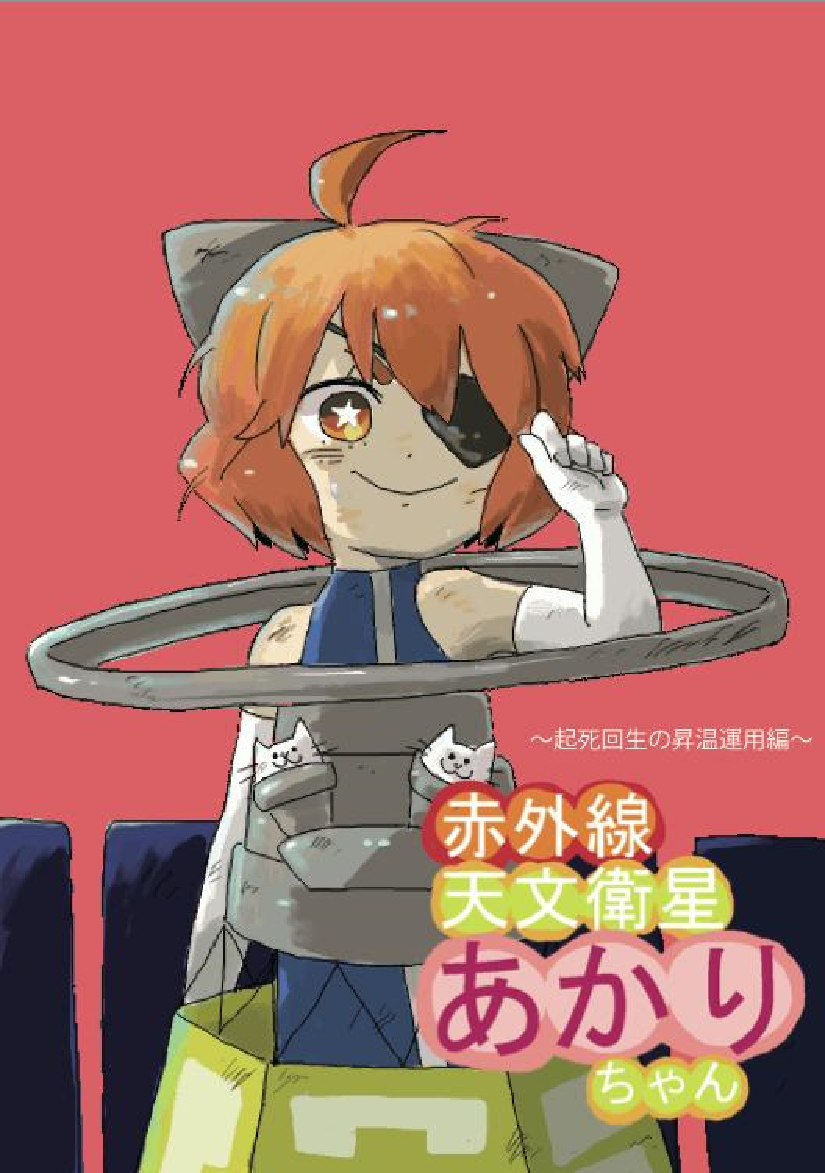
\includegraphics[width=60mm]{EPS/AKARIchan3.png}
}

\date{\Large{\bf March 13, 2015}}


\author{
  \Large{\bf 35-136359
  Aaron C. N. Bell}\\
 \begin{CJK}{UTF8}{min}\LARGE{ベル・アーロン・クリストファー}
  \end{CJK}\\[1cm]
  \Large{\bf Department of Astronomy}\\
  \Large{\bf Graduate School of Science,
  The University of Tokyo}\\
  \begin{CJK}{UTF8}{min}\LARGE{東京大学大学院理学系研究科}
  \end{CJK}\\
}




%%%%% main page %%%%%
\begin{document}

%%% make title %%%
\maketitle
\thispagestyle{empty}\mbox{}\newpage

\pagenumbering{roman}

%%% abstract %%%
\chapter*{Abstract}
\addcontentsline{toc}{chapter}{Abstract}
Rapidly spinning dust particles having a permanent electric dipole moment have been shown to be a likely carrier of the anomalous microwave emission (AME), a continuous excess of microwave flux in the 10 to 90~GHz range. Small grains, possibly polycyclic aromatic hydrocarbons (PAHs), are a leading suspect. In the absence of a definitive answer on the presence of PAHs or their role as an AME carrier, some predictions have been made as to the implications of spinning PAH emission. Due to the overlap between the CMB and the galactic foreground, this topic is requiring cosmologists to consider the ISM with more care. ISM astronomers are also needing to consider the contribution of cosmological radiation to large-scale dust investigations. We present data from AKARI/Infrared Camera (IRC) due to the effective PAH band coverage of its 9~$\mu$m survey to investigate their role within the 98AME candidate regions identified by Planck Collaboration et al. (2014). We supplement AKARI data with the four Infrared Astronomical Satellite (IRAS) all-sky maps and complement with the Planck High Frequency Instrument (HFI) bands at 857 and 545~GHz to constrain the full dust thermal spectral energy distribution (SED). We sample the average spectral energy distributions (SEDs) all 98 regions. We utilize all 7 AKARI photometric bands, as well as the 4 IRAS bands and 2 HFI. We carry out a modified blackbody fitting, and estimate the optical depth of thermal dust at 250~$\mu$m, and compare this to AME parameters. We also show plots of each band's average intensity for all 98 regions vs. AME parameters. We find a positive trend between the optical depth and AME. In the band-by-band comparison the AKARI 9~$\mu$m intensity shows a weaker trend with AME. In general, the MIR correlates less strongly with AME than the FIR. The optical depth vs. AME trend improves slightly when looking only at significant AME regions. Scaling the IR intensities by the ISRF strength $G0$ does not improve the correlations. A slightly positive trend found previously among 10 AME regions vs. AME significance is revisited, using the larger sample of 98. However the trend does not hold up to the full data set. We cannot offer strong support of a spinning dust model. The results highlight the need for full dust SED modelling, and for a better understanding of the role that magnetic dipole emission from dust grains could play in producing the AME. 

%\include{jabstract}

%%% table of contents %%%
\tableofcontents
%\listoffigures
%\listoftables
\listoffigures
%%% main chapters %%%
% Empty pages are inserted to make each title page
% come to the right-hand side (odd page) of the book.

%%% page numbering %%%
\pagenumbering{arabic}

\chapter{General Introduction\\
\label{chap:Introduction}}

\section{A Quick Dive into the Interstellar Medium}
The Interstellar Medium (ISM) is complicated. 

The ISM pervades the galaxy and either surrounds or intervenes basically any object one may wish to study. The pristine, primordial ISM is the reservoir which all present material in our universe was formed from, and the ISM is enriched as matter is processed and flows back into space.

In a simplistic way we can describe the ISM as a mixture of gas and dust. An early estimate by \cite{knapp74} puts the mass of dust in the galaxy at about 1\% that of interstellar gas. In the march forward of interstellar medium inquiry since the early efforts to understand the material responsible for the extinction of starlight, many new species of interstellar dust have been modelled and discovered.  The modes by which these dust species interact and evolve are also beginning to be understood. However there are many questions left to answer and even now our understanding of dust emission, interaction, and evolution, continues to evolve.

The study of dust has been connected to mainstream astrophysics research, and recognized as an integral part of the interstellar medium. This has been shown by early sounding rocket experiments \citep{wolstencroft67,soifer71}, and balloon experiments \citep{muehlner70,emerson73}, and dust has been more profoundly exposed by the advent of all-sky infrared surveys like the  Cosmic Microwave Background Explorer's Diffuse Infrared Background Experiment (COBE/DIRBE) \citep{sodroski94} and the Infrared Astronomical Satellite (IRAS) \citep{iras84}. With space-borne long-term IR mapping finally available on an all-sky scale, we could move past the interplanetary medium and into the interstellar.

The role of dust in the interstellar medium has expanded beyond simply an intervening, stellar light obstructing material. Theoretical models and observations have shown that dust grains act as a catalyst for the formation of molecular hydrogen and other molecules, providing a substrate upon which hydrogen and other atoms can meet \citep{iglesias77,burke83}. With infrared observations we are able to study dust directly via its vibrational emission, rather than relying only on inference from visible reddening and polarization effects \citep{davis51,platt56, carrasco73}.

  A wealth of data is availablr in the infrared to sub-millimeter range and the interpretation of this data has become a serious priority. This is especially true for the last ten years as new, much higher resolution surveys have been carried out such as the Spitzer Space Telescope \cite{spitzer04}, Herschel Space Observatory (Herschel) \citep{herschel10} by NASA and the ESA respectively, and the AKARI telescope \citep{akari07},  by JAXA. AKARI especially, produced a wealth of data spanning the entire sky. It was equipped with IRC \citep{irc07} to study the MIR, and FIS \citep{fis07} to study cooler dust and gas, and conduct spectroscopy in the far infrared (FIR) via its built-in Fourier Transform Spectrometer (FTS). The FIS all-sky maps have just been publicly released at the time of this writing (Doi, et al. 2014). The IRC all-sky maps are soon to follow. In this thesis we use these AKARI surveys in a comparison with other cutting edge all-sky maps from the Planck Observatory in a multi-wavelength study of yet another part of the ISM puzzle, the AME and its connection to interstellar dust.
 
%%%% Citation needed for early dust revelation work%%%


%%%%%%Citation for the modeling of hydrogen condensation%%%
%%%%%%Citation for observations showing that dust traces heavy star formation%%%%%

\section{What is dust made of}

The question of the composition of dust has grown from a single thread of investigation into a network of questions. Many pieces in this dusty puzzle are missing. For example, the presence of dust grains containing silicates, and amorphous carbon is very strongly supported by comparisons of infrared spectroscopy with laboratory studies \citep{hagen79,joblin09}. But many questions remain about which silicate and carbonaceous species may be present, and in what proportions, and in what distribution of sizes. The question also remains, is there more to dust than simply carbonaceous and silicate grains?  The exact size distribution of dust grains is also an open question. The composition of extremely small grains / large molecules is a particularly challenging mystery, as well as the role of interstellar ices in the evolution dust and gas.

\subsection{Silicate Grains}
     One of the first materials proposed to exist as interstellar dust were silicates, with the first evidence being UV absorption features \citep{knacke69}. More recently, specific species of silicates are being identified via absorption spectroscopy \citep{olofsson12}. However some doubt has been cast recently on the structure of the grains. For example, in \cite{jones13} and \cite{jones14} an updated model is proposed wherein dust grains may be composed of a mixture of silicate and amorphous carbon material, such as a silicate core with an amorphous carbon envelope. Figure \ref{Jones Dust} provides a diagram of the dust composition scheme suggested by the \cite{jones14}
 model. Note the core and mantle structure of the silicate grains. An additional feature of this model is that silicates having iron inclusions are expected, which would be similar to the Fe form of olivine.
      This is an update from the conventional ``astronomical  silicates" assumed in earlier dust spectral energy distribution (SED) models such as \cite{li01} or \cite{dustem11}.

\begin{figure}[htbp]
\begin{center}
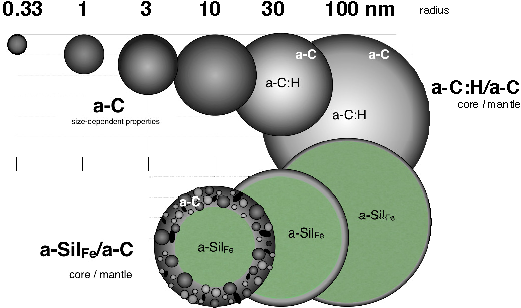
\includegraphics[width=150mm]{EPS/aa21686-13-fig1.pdf}
\caption{
In image from \cite{jones14} demonstrating a newly proposed model for dust composition, and showing that the dust story is far from concluded. a-C denotes amorphous carbon; a-C:H, hydrogenated amorphous carbon (HAC); a-Sil, amorphous silicon. The main point of the model is to propose that a mixture of amorphous carbon, amorphous silicates, and aromatized carbon is still supported but with an updated distribution of grain structures (some silicates may have amorphous carbon mantles) and updates to the typical size distributions. They propose a continuous distribution of grain structure from individual PAHs to amorphous carbon grains having an aromatized envelope, to silicates, to silicates with aromatic and/or amorphous carbon envelopes.
 }
\label{Jones Dust}
\end{center}
\end{figure}
\subsection{Carbonaceous Grains}
     As with silicates, it is well-established that carbonaceous material, primarily amorphous carbon, exists in the ISM \citep{aitken81,tielens87}. This is material commonly called ``soot" or the fuel we know on earth as coal.    Some non-amorphous carbonaceous material is also speculated to exist, such as graphite \citep{zhou06} or ``buckyonions" (concentric-shell-graphite) \citep{li08}. Even diamond has been proposed to exist in the ISM \citep{tielens87}, and has been discovered within meteorites thought to contain pre-solar material \citep{anders93}.
%\begin{figure}[htb]
%\centering
%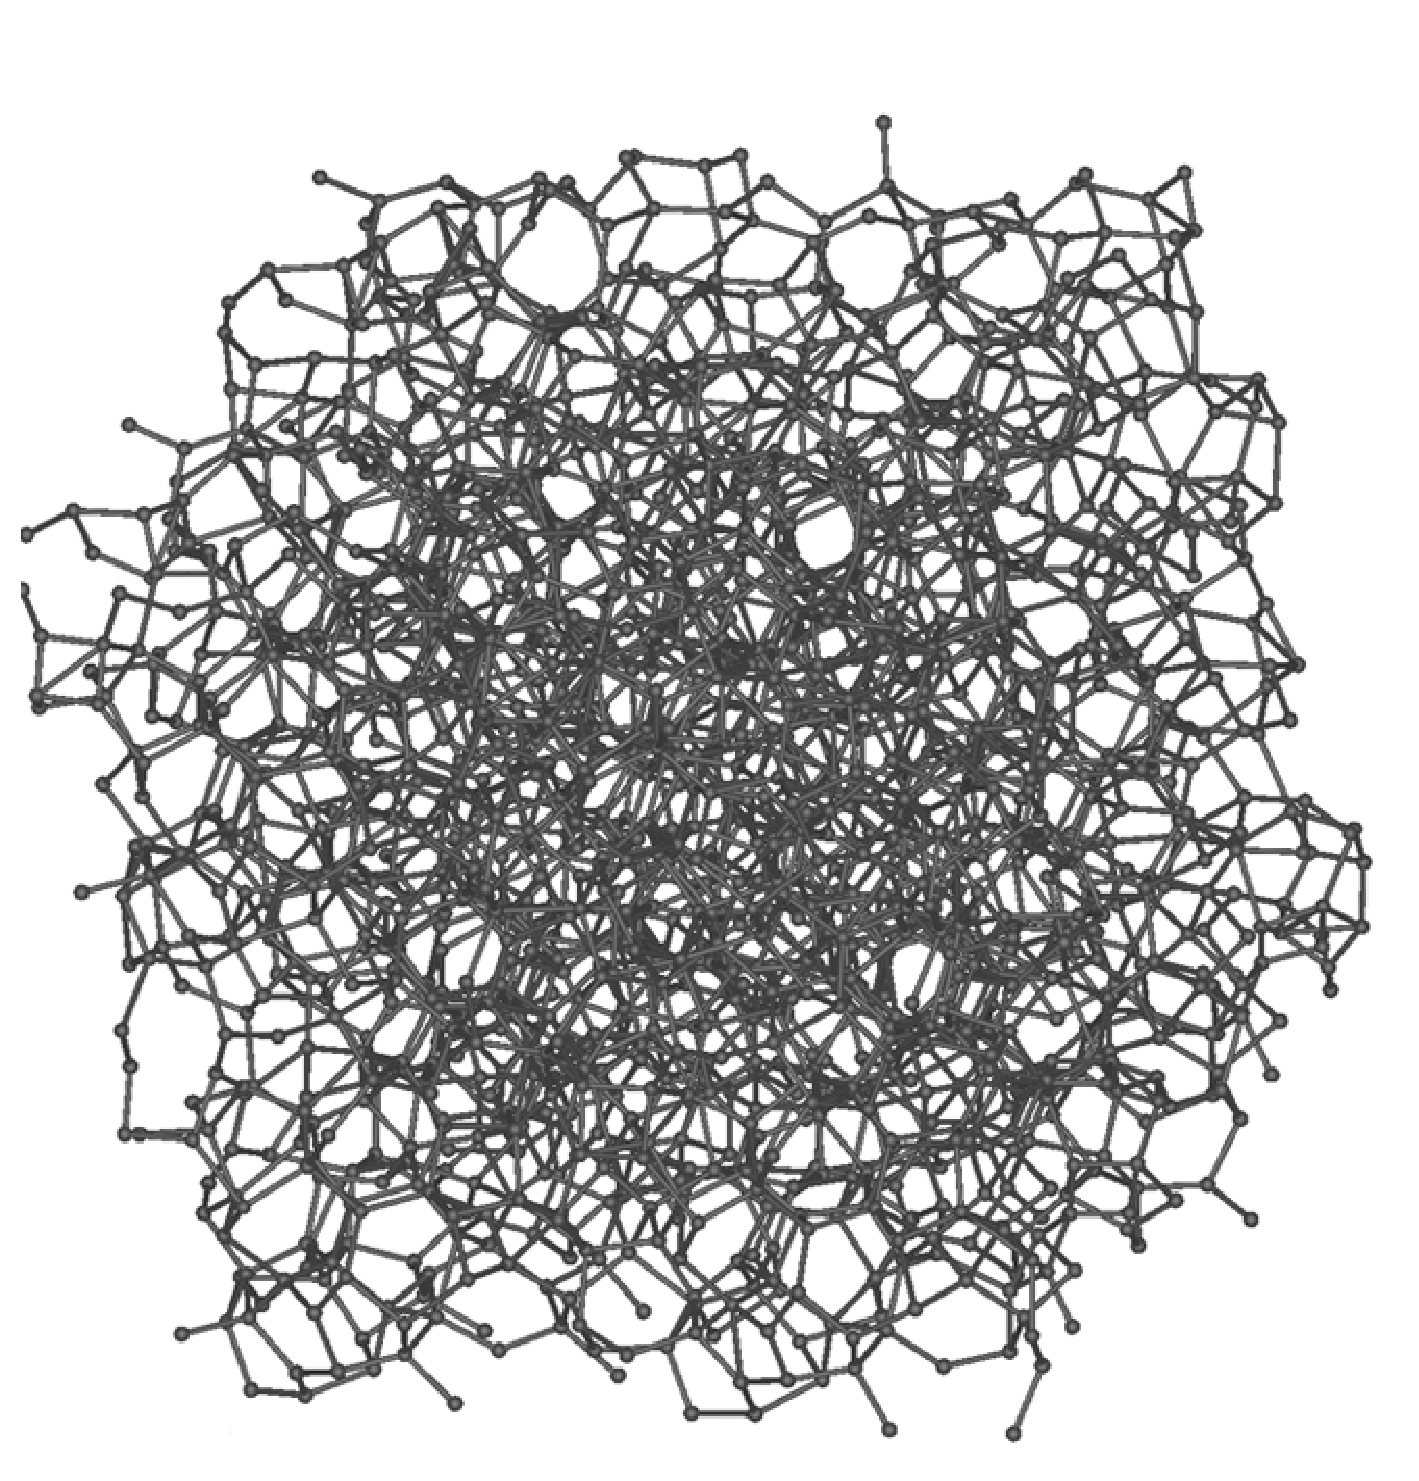
\includegraphics[width=100mm]{EPS/Amorphous_Carbon.pdf}
%\caption{
%Creative-commons image depicting the typical structure of amorphous carbon. The lack of an organized structure %leads to variations in the vibrational spectra.
% }
%\end{figure}
%%%%Ant Jones Figure???%%%
\subsection{The PAH Hypothesis}
\label{PAHhypothesis}
     Over the years since we have been studying interstellar material, the composition of dust has been debated heavily. 
     Within  the last 30 years, a popular hypothesis has arisen that a particular set of features of the interstellar medium SED between 3 and 12 microns, known as the ``Unidentified Infrared Bands" (UIRs), can be explained by the PAH family of molecules. The PAH interpretation was first proposed by \cite{allamandola85} and \cite{puget85}.
     With the appearance of high powered computers with an ability to perform rigorous calculations, many attempts have been made to simulate the expected emission from PAHs. Density functional theory (DFT) \citep{honenberg64} has become available as a tool for simulating molecular emission features using a quantum approach. DFT calculations has become a subfield of ISM astrophysics. Many attempts are being made to fit particular emission features of PAHs, and other molecular and grain species, to observed ISM features \citep{hammonds09,hirata99}.
     While it is difficult to reproduce the exact interstellar conditions in a laboratory setting, DFT simulations have yielded some evidence that the UIR bands can be explained as PAH vibrational emission features \citep{pathak12,ricca11,yu12}.

Some recent evidence by \cite{zhang14} has shown theoretically that mixtures of non-PAH carbonaceous and silicate spectra could also fit the theoretically calculated PAH emission features. However the PAH-UIR hypothesis is still widely supported \citep{tielens08,rastogi13}. The way that PAHs might be produced or evolve from other species is not understood however. Though there are efforts underway to model potential formation pathways. As far as the evolution of larger aromatics form smaller PAHs, there is one proposed pathway wherein a benzene could grow into a larger aromatic molecule such as naphthalene \citep{ghesquiere14}.

%%%Ahmit says Gillet is the first citation... GIllet 1973. But Allamandola 85 and leger 84 attributted them 戸PAHs。
%%% Or\cite{allamandola89}.???? %%%
%%%Existence of PAHs is being supported by DFT calculations matching observations. However there is some suggestion recently that other chemistries could produce the PAH bands, but this is not yet confirmed.
%%%Difficult to confirm PAH spectra in the laboratory, because difficult to get them into the gas phase as they would be in space.
%%%%Ahmit produced a thermal emission model ot the PAHs assuming some incident ISRF. See Pathak and Rastogi Temperature of the PAH will decrease in steps.
%%%PAHs are stable. The formation of the first ring may not be well understood, there is not experimental understanding of that step. The process of adding rings once the first is formed is more well understood. Pathway proposed where PAHs could serve as a substracte for the H2 formation. Adding of rings is well understood theoretically and experimentally. Another way to call the PAH bands is the aromatic infraared bands. Remember that PAH includes a wide class oof things. It is a molecule family. May be clusters of PAHs, inoized as well as neutral PAHs, and with chemical substitutions. PAH gives the whole family. It seems very clear that they would give the UIR bands.-Ahmit via Richter and Howard and Frank Klack
%%Don't forget to discuss the PAHs with respect to vibrational emission, and the way that multiple bands are produced from one UV excitation. 1E-6 second timescale for UV absorption to IR emissin -Ahmit. The fluorescene timescale is much longer. 
%%%Is there a referse process? Yes, for equal levels. Remember that a transition back to the ground state can also occur, producing a UV or visible photon.
%%%%Jones et al. 2014%%%%
\section{Galactic Microwave Foreground}

For astronomers wanting to study the microwave sky for cosmological purposes, there are foreground components which must be accounted for. These components arise from the simple reality that we are observing from inside the Milky Way. Our galaxy, and other galaxies, produces microwave emission which overlaps with frequencies important for the cosmic microwave background (CMB).

\subsection{Thermal (Vibrational) Dust Emission}
%%%Insert IRAS 100~$\mu$m or other plot showing the global dust emission%%%

In the optical, dust is interference. In the infrared, it is bright. The direct emission from dust, via thermal equilibrium vibrational modes, dominates in the far infrared (this is different from the stochastic heating and emission expected from very small grains, see Figure \ref{Transient heating of small grains}).

Assuming only emission by the vibrational modes, \cite{draine99} gives the power radiated per grain per frequency increment, $P_{\nu}d\nu$ as:

\begin{equation}
\label{spinpower}
P_\nu d\nu = 4\pi C_{abs}(\nu) B_\nu(T)
\end{equation}
where $B_{\nu}(T)$ is the Planck function per frequency, and $C_{abs}$ is the absorption cross-section at $\nu$.

\begin{figure}[htbp]
\begin{center}
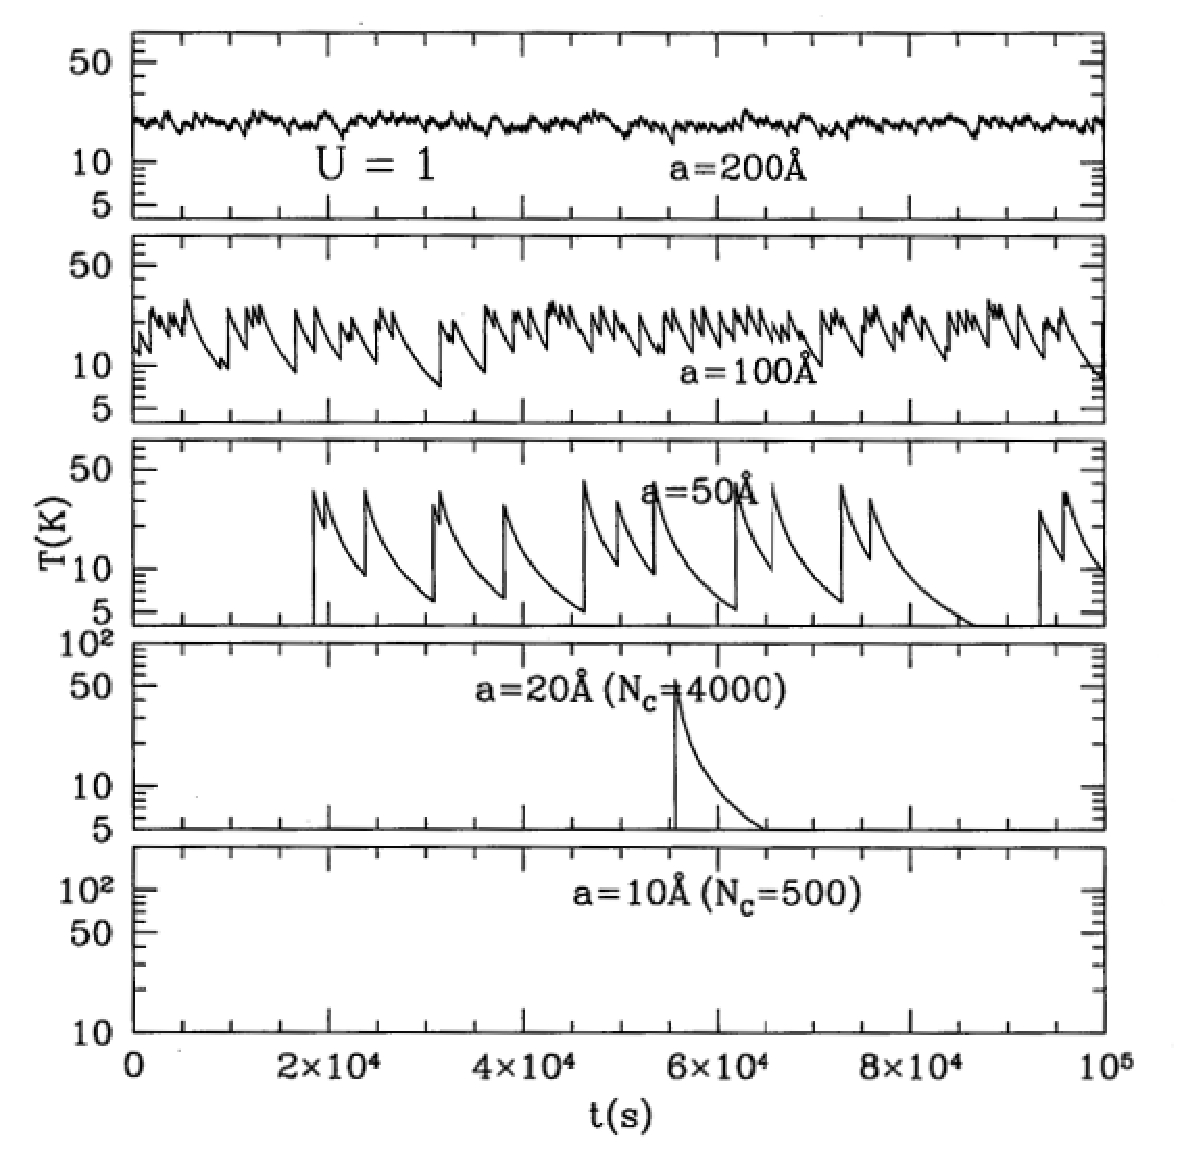
\includegraphics[width=150mm]{EPS/one-photon_heating.pdf}
\caption{
This diagram \cite{draine11} showing the heating and cool-down times of grains of various sizes. This example assumes a carbonaceous grain, and a radiation field equal to that of the solar neighborhood (U=1). Most importantly, note the lower plots: a grain of size 20 angstroms is heated and cooled very quickly. This is because when a grain is small enough, its heat capacity becomes close to the energy absorbed by an incident UV photon. They heat up very quickly; cool down very quickly. The top plot, for size 200 angstroms, shows that the grain temperature undergoes only small fluctuations.
 }
\label{Transient heating of small grains}
\end{center}
\end{figure}
%%%insert that figure describing grain temperature distributions%%
Though the exact shape of the dust SED for grains in thermal equilibrium varies across environments, and is not completely understood, it is well-approximated by a modified blackbody curve, as used in \cite{onaka99}. A modified blackbody simply means that a modification of the frequency dependence is applied to the Planck Law intensity, given below. For a blackbody, the intensity is proportional to the frequency, $\nu$ squared times the spectral radiance  per frequency, $B_\nu$ as a function of temperature, $T$.
\begin{equation}
I(\nu) \propto B_\nu{}(T)
\label{BBintensity}
\end{equation}
The intensity of a modified blackbody is given by the same proportionality above, but with a modification of the power law steepness. Thus the intensity of thermal dust emission, $I_d$ is given below. 
\begin{equation}
I_d(\nu) \propto \nu{}^{\beta{}_d}B_\nu{}(T_d)
\end{equation}
where $\beta$ is known as the ``emissivity index". The value of beta may vary, and the nature of these variations is a topic of intense discussion \citep{galliano11,juvela12}, but is commonly around 2.0 $\pm$ 0.5. The result of augmenting the blackbody with $\beta$ is such that a peaked continuum is still present, though the steepness of the SED is changed. 
%%%%insert citation for modified blackbody fitting and equation%%%
     This curve extends into the microwave realm, and if the amplitude is high enough, it may significantly overlap with other microwave sources. This is not a mysterious process, simply the microwave extremity of the well-studied infrared thermal emission process.
%%%%insert figure generated from Fred's code...show the modified BB fitting extended into the 30 GHz range%%
\subsection{Thermal Bremsstrahlung (Free-Free Emission)}
     Ionized gas in the galaxy will emit microwave radiation as the free electrons are accelerated. This becomes significant for foreground HII regions, and even more so for ultra-compact HII regions (UCHII). Free-free emission may be traced by H$\alpha$ surveys, as ionized hydrogen regions throughout the galaxy are thought to be the primary source of the galactic free-free foreground. Spectrally, free-free emission appears to follow a power-law distribution (related to the velocity distribution of the electrons in an ionized cloud). The typical value of the free-free spectral index, $\alpha$ is ~-0.13. However the exact separation of free-free emission from other galactic microwave foreground components is difficult, as the  frequency range 10 to 90 GHz overlaps with several galactic components \citep{wmap03b, leach08, planckXII}.
%\begin{center}
%\begin{equation}
%j_{ff,\nu}=\frac{8}{3}(\frac{2\pi}{3})^{1/2}g_{ff,i}\frac{e^6}{m^{2}_{e}c^{3}}
%(\frac{m_{e}}{kT})^{1/2}e^{\frac{-h\nu{}}{kT}}n_{e}Z^{2}_{i}n_{i}
%\end{equation}
%\end{center}
\begin{figure}[htb!]
\begin{center}
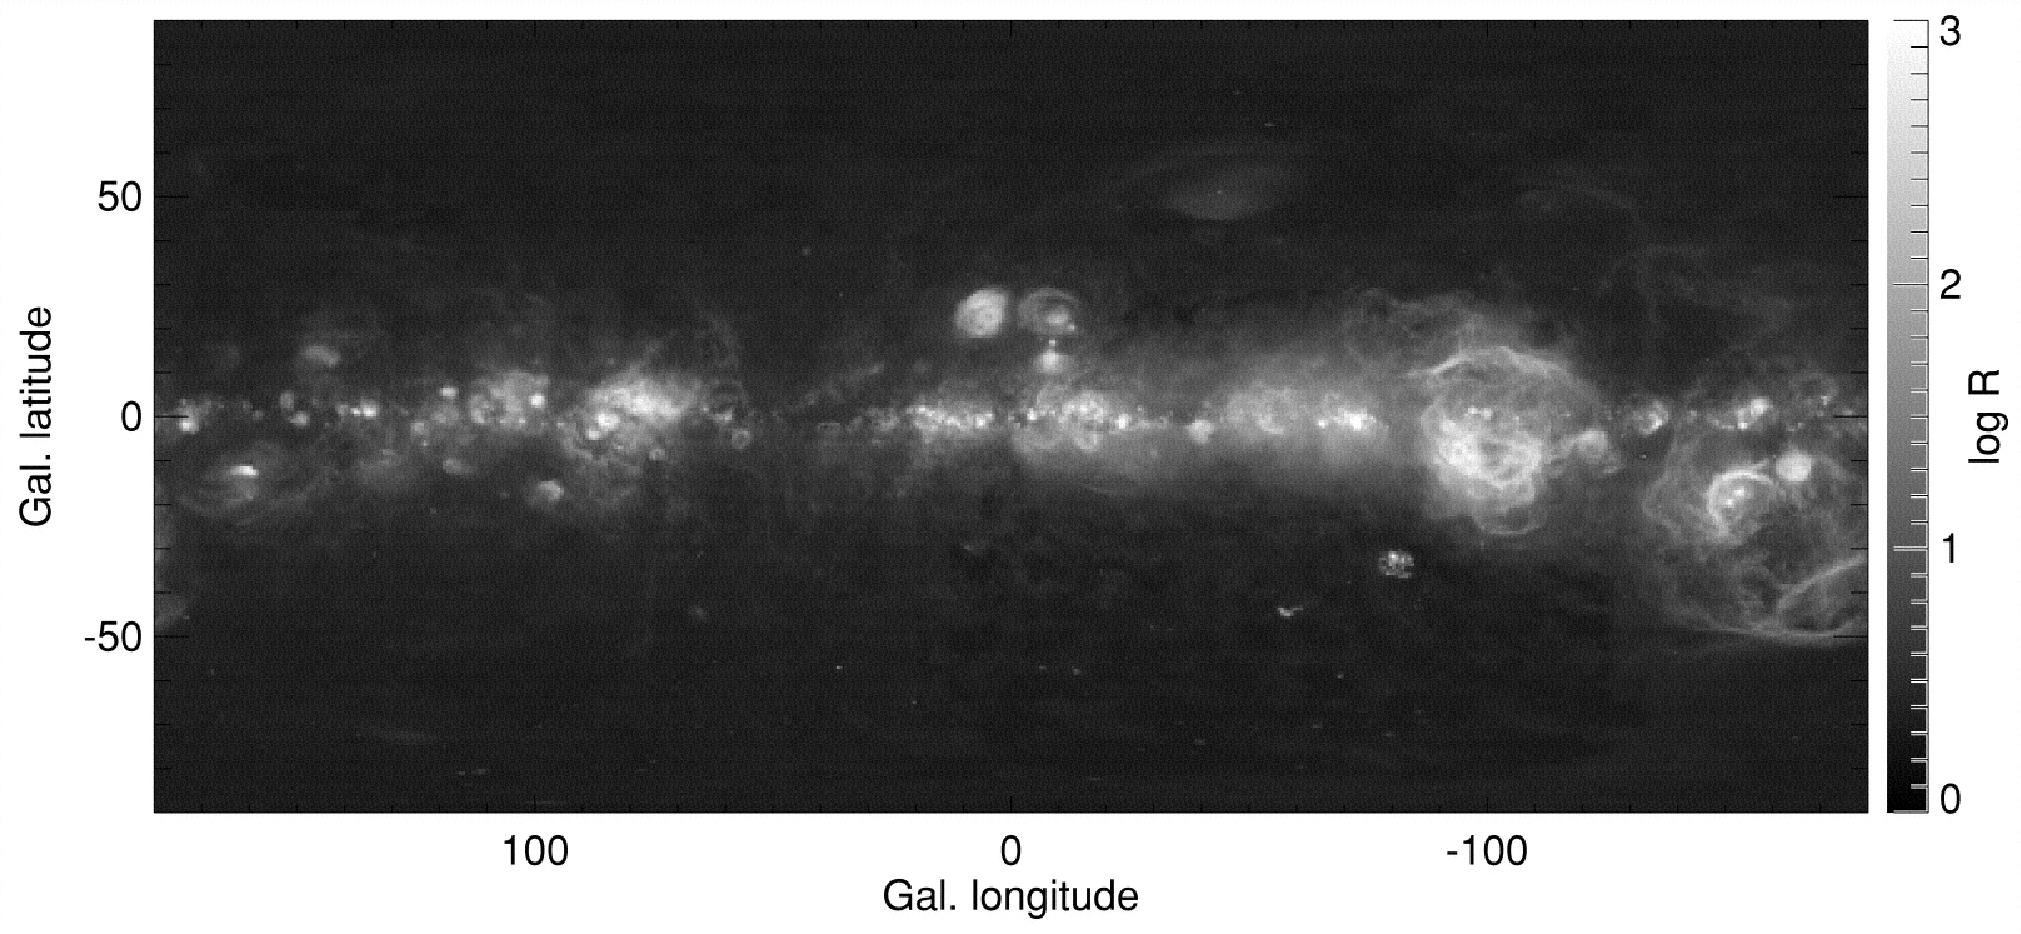
\includegraphics[width=150mm]{EPS/finkbeiner03_fg4_halpha.pdf}
\caption{
This is a template of H$\alpha$ emission for the galactic foreground, created by \cite{finkbeiner03}, derived from observation by the Wisconsin H-alpha Mapper (WHAM) \citep{wham98}, the Virginia Tech Spectral-Line Survey (VTSS) \citep{dennison98}, and the Southern H-Alpha Sky Survey Atlas (SHASSA) \citep{gaustad01}. The map is shown in galactic coordinates, and the greyscaling corresponds to the brightness in rayleighs ($1~R = 795.775\times10^6 [photons·m^{-2}·sr^{-1}]$). In their work, they describe that free-free emission should be well-traced by the amount of H$\alpha$, since free-free is produced from ionized gas clouds. However a free-free map is difficult to produce, since H$\alpha$ is an electronic emission feature and thus readily absorbed by intervening ISM. In order to derive the free-free contribution, the absorption of H$\alpha$ by dust must be corrected for. Estimating the free-free emission contribution is a critical step in order to isolate anomalous microwave emission.  
 }
\label{Dust}
\end{center}
\end{figure}

The free-free emission foreground has been studied extensively due to its relevance to (interference with) CMB investigations. In fact, attempts have been made to explain anomalous galactic foreground components via excess free-free emission \cite{kogut96}.

\subsection{Radial Bremsstrahlung (Synchrotron Emission)}

Driven by the Milky Way’s magnetic field, relativistically accelerated charged particles emit synchrotron radiation. The spectral shape of this radiation is very flat and predictable. Though it is not strongest in the microwave range, synchrotron emission is a significant foreground radiation field even at wavelengths around 30~GHz. 

When studying other microwave sources, we can control for synchrotron emission by looking at a less crowded frequency such as at 408~MHz. Figure 1.4 shows the radio survey by \cite{haslam82}, which is a useful tool for separating synchrotron emission from the AME, where synchrotron emission is the dominant component. From this lower frequency information the synchrotron flux density contribution,$S_{\rm sync}$, can be extrapolated to a target microwave frequency, $\nu$, using the following equation:

\begin{equation}
S_{\rm sync} = A_{\rm sync} \left( \frac{\nu}{{\rm GHz}}\right)^{\alpha}~
\label{synchrotron}
\end{equation}

This is the method used by \cite{planckXV} (hereafter, PCXV), where $A_{\rm sync}$ is the power law amplitude, $\alpha$ is the spectral index (having a typical value ~-3).
  
\begin{figure}[htb!]
\begin{center}
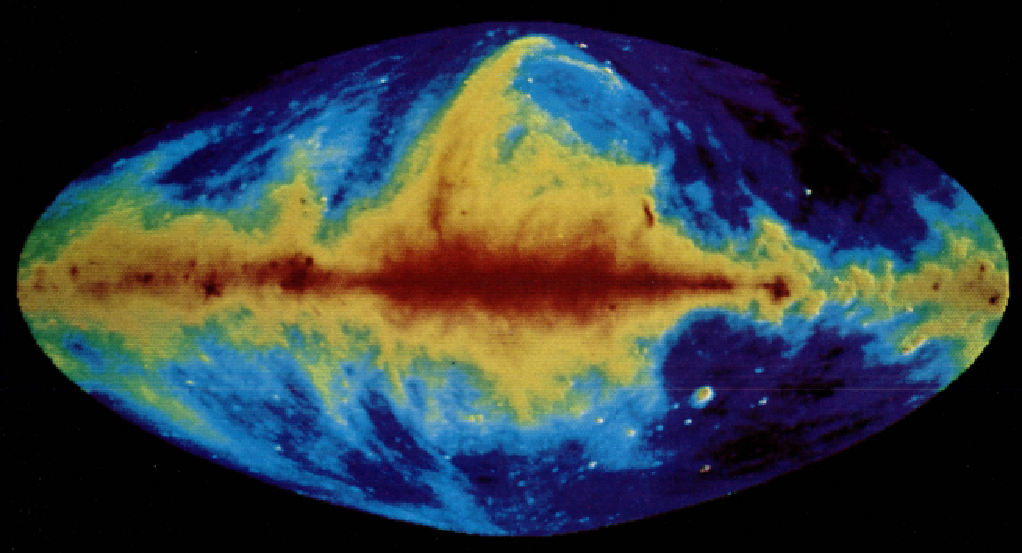
\includegraphics[width=150mm]{EPS/haslam403.pdf}
\caption{
408~MHz all-sky survey by \cite{haslam82}. The galactic foreground at this frequency is largely dominated by synchrotron emission. 
 }
\label{Dust}
\end{center}
\end{figure}

\section{Anomalous Microwave Emission}
%\label{sec:introduction:background}}
     Upon its first detection in early microwave surveys \citep{leitch97}, the AME or  ``Foreground X" \citep{deoliveiracosta02}, has been found to be a widespread feature of the microwave SED. That is, it appears over a very large portion of the sky. However its signature generally follows that of the galactic foreground of the Milky Way. The AME is almost certainly of galactic origin (we do not address the topic of AME in other galaxies, however a submm-mm excess has been noted been noted in the SMC, and attempts have been made to explain it as magnetic dipole emission, a similar process \citep{draine12}). Beyond the Milky Way-AME correlation however there is still much mystery, except that the most likely source of the AME is interstellar dust. \cite{kogut96,deoliveiracosta97,leitch98} showed that the AME correlates very well with dust, via the IRAS 100~$\mu$m surveys.
     Subsequently, \cite{ysard10b} compared the AME sky as revealed by WMAP \citep{wmap03a} to IRAS all-sky maps (see \ref{ysardcorrel}. They found a tighter correlation with dust at 12~$\mu$m than at 100~$\mu$m, implicating small dust (stochastically emitting dust). See Figure 1.2 for a description of the stochastic small grain emission, which was well-described by \cite{draine01}. 100~$\mu$m emission is produced by the larger, classically heated dust grains. More recently, using the cutting-edge Planck data, PCXV made a similar AME vs. IRAS comparison to that of \cite{ysard10a}, finding a similar result; IRAS 12~$\mu$m correlates more strongly with AME than IRAS 100~$\mu$m (see Figure 1.6).

\begin{figure}[htbp]
\begin{center}
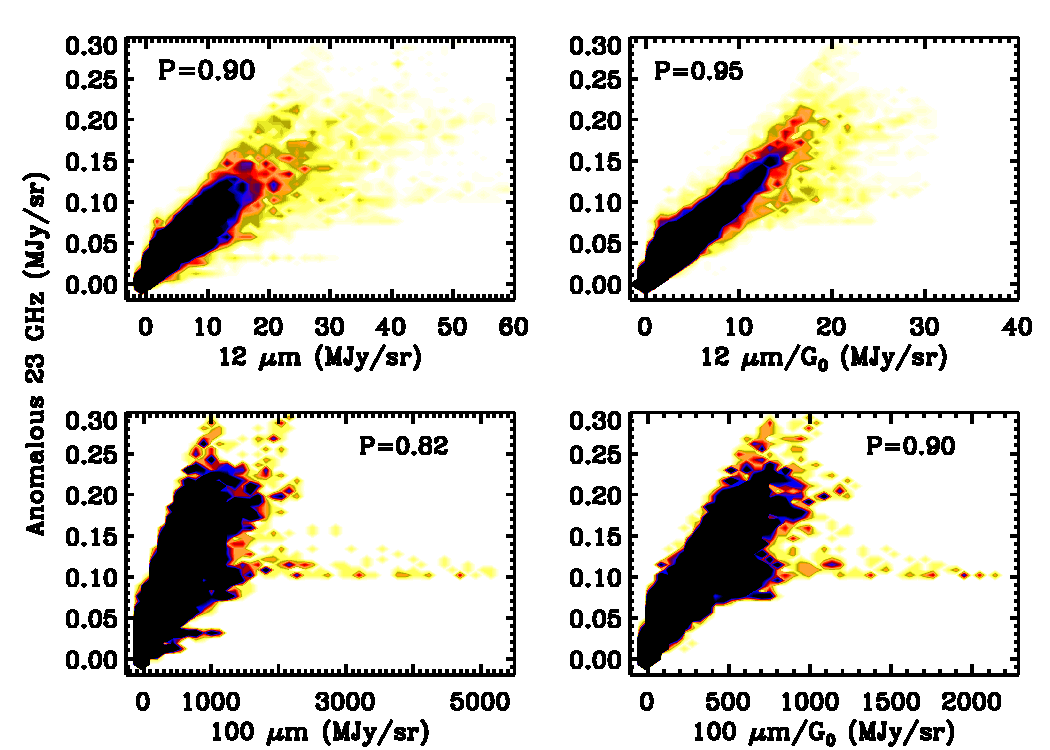
\includegraphics[width=150mm]{EPS/correl_ciel.pdf}
\caption{
A correlation test of AME (via WMAP) vs. thermal dust emission (via IRAS). Quoted from \cite{ysard10b}. The panels at left show simply the AME intensity at 23~GHz plotted against the IR intensity at 12~$\mu$m which traces mostly small grains (top), and 100~$\mu$m which traces mostly grains in thermal equilibrium (bottom). At right, the same data is plotted though with the IR intensities having been scaled by $G0$ value at each point. $G0$ is the intensity of the interstellar radiation field vs. that of the solar neighborhood. The correlation is stronger at 12~$\mu$m vs. 100~$\mu$m ($P=0.90$ vs. $0.82$). Both correlations improve slightly after scaling by $G0$.
 }
\label{ysardcorrel}
\end{center}
\end{figure}


\begin{figure}[tb]
\begin{center}
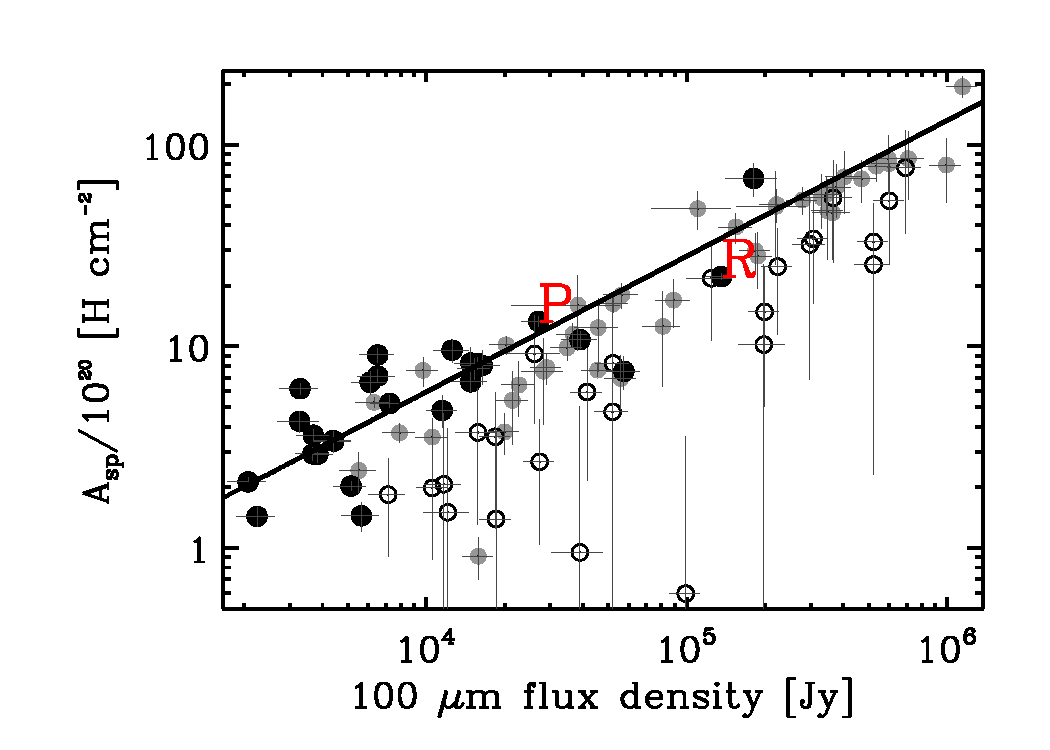
\includegraphics[width=0.45\textwidth]{EPS/fig18_1.pdf}
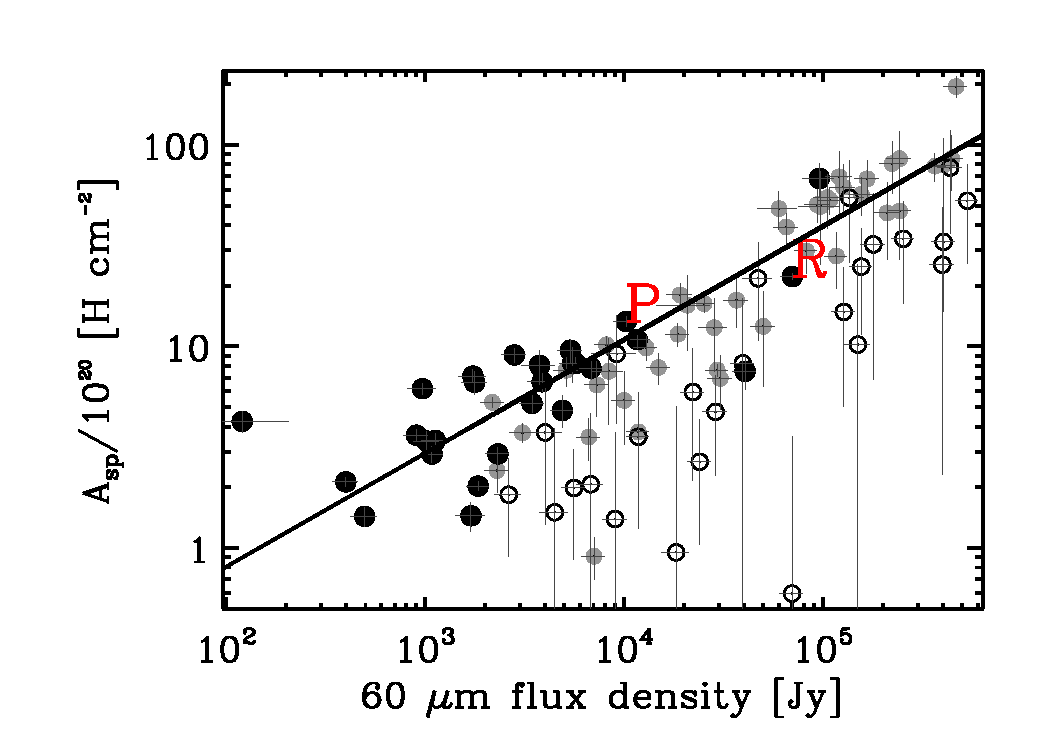
\includegraphics[width=0.45\textwidth]{EPS/fig18_2.pdf}
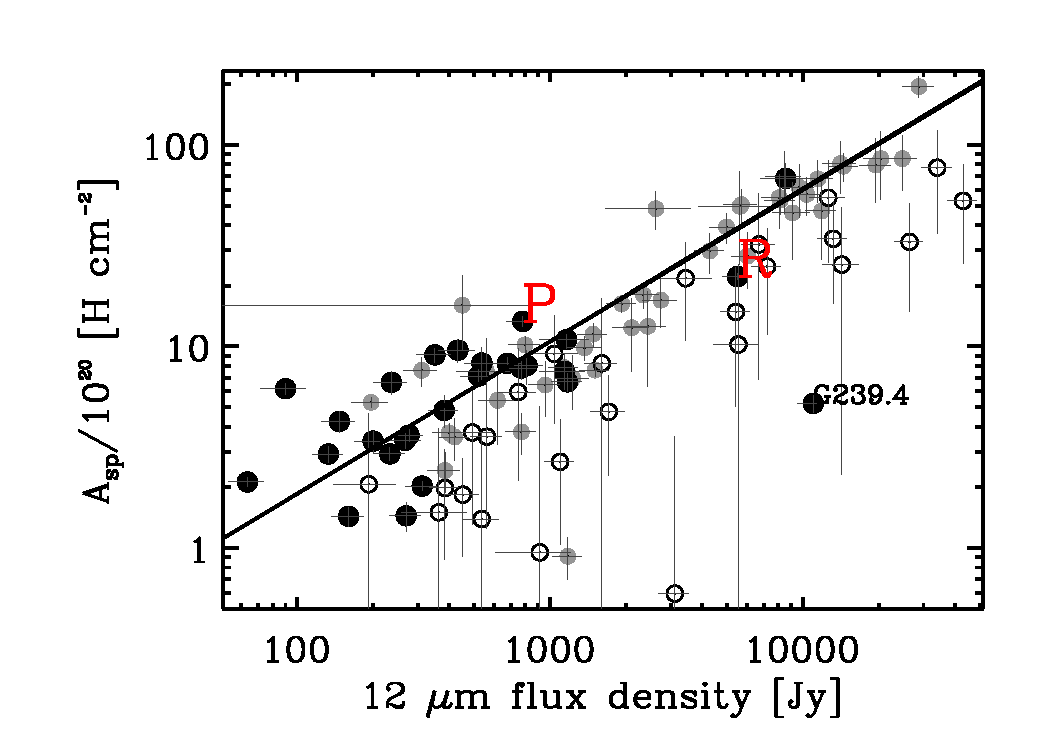
\includegraphics[width=0.45\textwidth]{EPS/fig18_3.pdf}
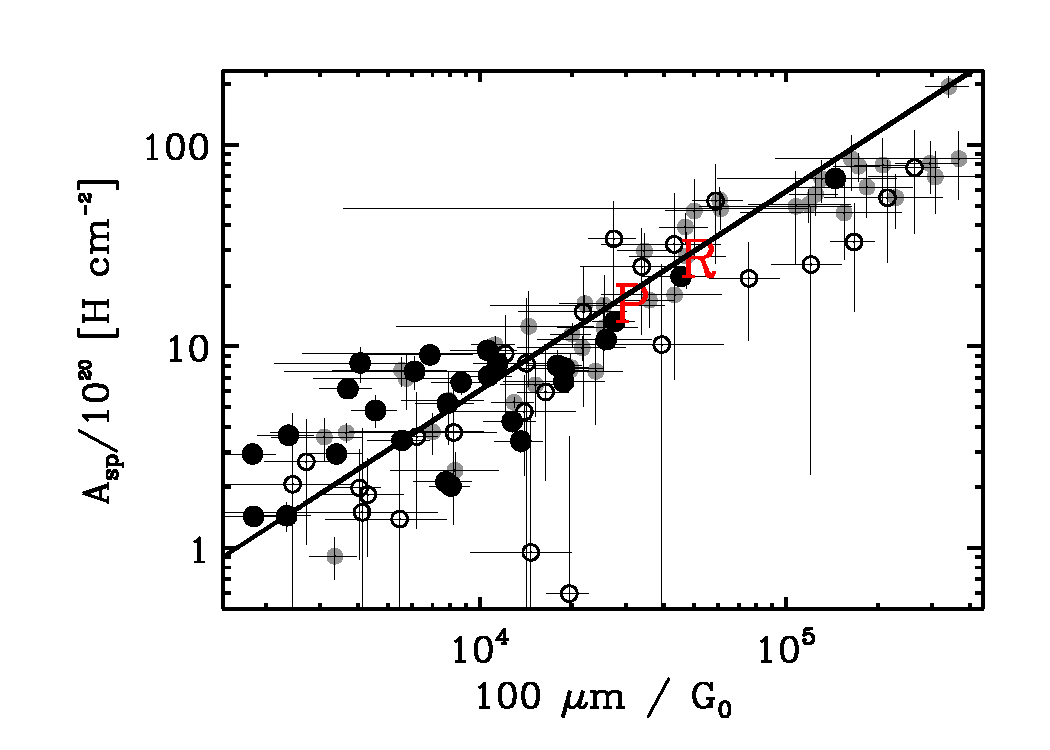
\includegraphics[width=0.45\textwidth]{EPS/fig18_4.pdf}
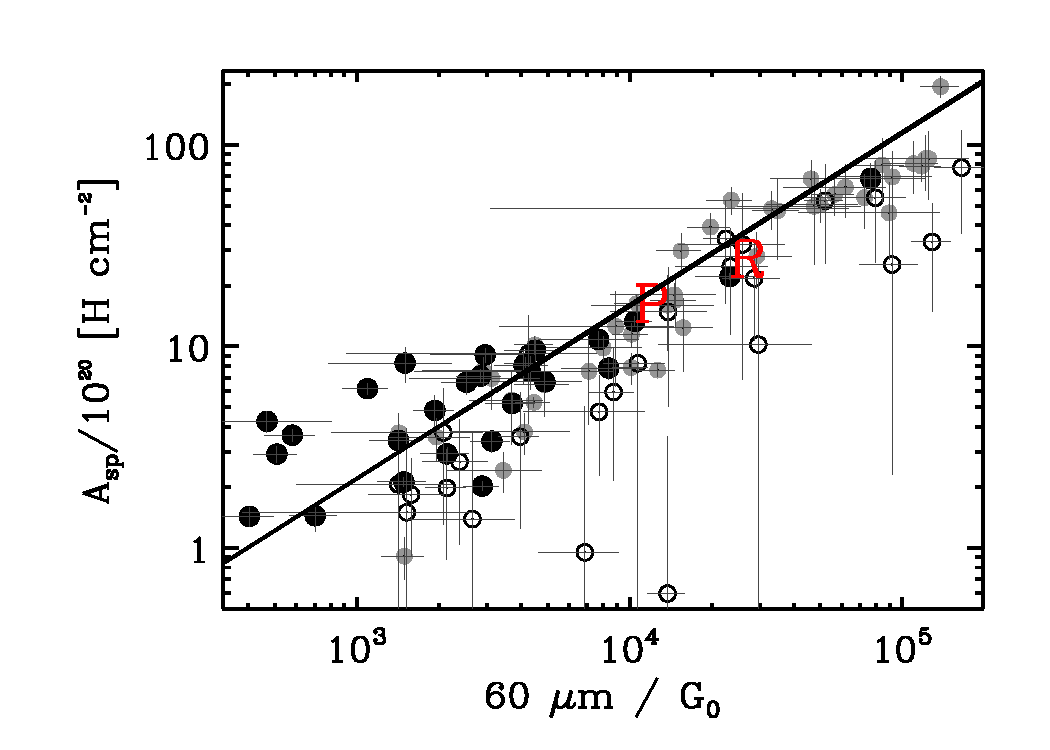
\includegraphics[width=0.45\textwidth]{EPS/fig18_5.pdf}
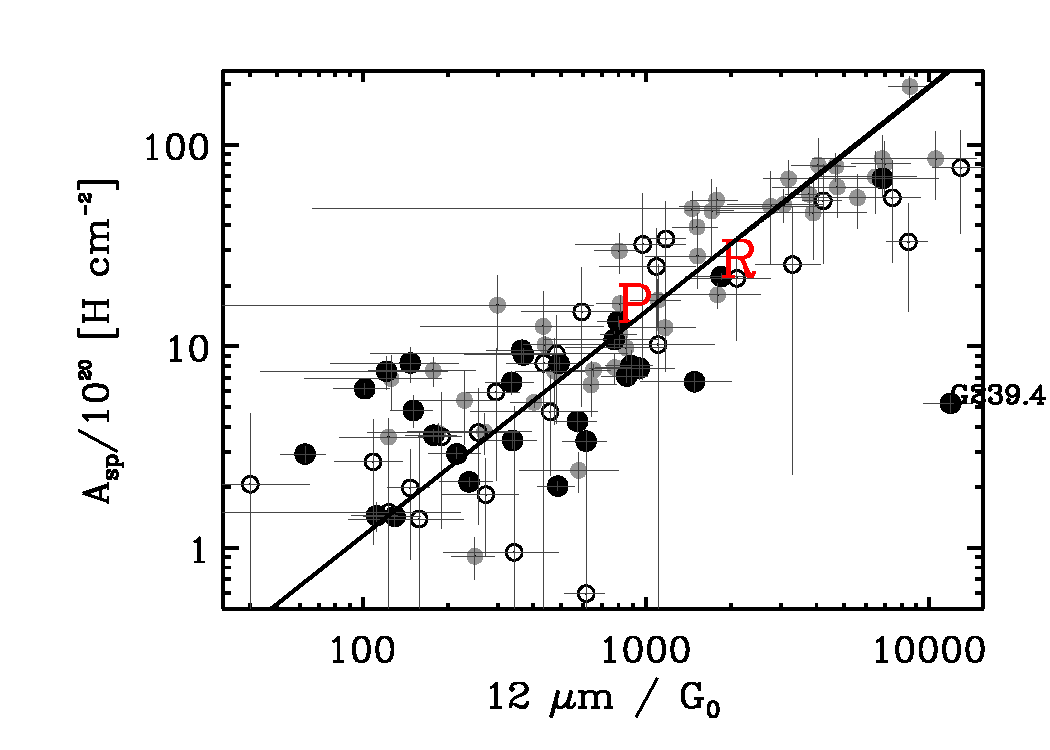
\includegraphics[width=0.45\textwidth]{EPS/fig18_6.pdf}
\caption{Dust Correlations from \cite{planckXV}, based primarily on Planck LFI \citep{lfi14ii} microwave data and IRAS IR data. The top 3 plots show the AME amplitude (which is \textit{``roughly equivalent to the column density of spinning dust, assuming there is no shift in peak frequency"}, according to \cite{planckXV}) vs. the total flux density [Jy] at the IRAS IR wavelengths of 12, 60, and 100~$\mu$m. Their flux densities were summed over a 1$\degree$ radius circular aperture (after smoothing the data to 1$\degree$ resolution}
\label{planckcorrel}
\end{center}
\end{figure}
     We once thought emission in the 10 to 90~GHz frequency domain was sourced by a combination of the cosmic microwave background (CMB), free-free emission, and synchrotron radiation. The RING5M CMB experiment in the 1990s cast some doubt on this explanation when excess microwave flux was detected near the north celestial pole by \cite{leitch98}. They describe that although the CMB contributed 90\% of their extracted signal: \textit{``Our 14.5 GHz observations of the NCP have also resulted in the detection of an anomalous component of Galactic emission [...] a cautionary tale for future CMBR experiments."}
     AME has been shown to take the shape of a ``sub-millimeter bump”, an excess over the expected free-free and synchrotron emission. The peak of this bump is typically around 30~GHz (PCXV). Given the typical spectrum and its peak frequency, PAHs have been proposed as a likely carrier of the AME. PAHs which are rapidly spinning and which have a permanent electric dipole should produce microwave emission. However there is a secondary explanation, the possibility of a contribution from magnetic dipole emission (these will be explained in more detail in the following sections). These two mechanisms are not mutually exclusive, and the spectrum of magnetic dipole emission has also been theoretically determined by \cite{draine99}. They report that this emission should overlap with spinning dust emission.
     As the microwave sky was revealed in more and more detail, the anomaly became more of an unexplained galactic foreground component. AME was detected not only towards the NCP, but in several prominent regions which were not expected to show bright microwave emission. The $\rho$ Ophiuchi molecular cloud is one of these \citep{casassus08}. 
     This microwave foreground has been studied extensively since then. AME has been correlated with thermal dust emission, leading to the suggestion that AME is electric dipole emission from spinning dust \citep{draine98b}. All-sky comparisons between WMAP and IRAS maps further support the correlation with the Milky Way, and with dust. The 100 micron (3~THz) IRAS map correlates well with the AME, and more interestingly the 25 micron maps shows an even tighter correlation \citep{ysard10a}. One implication of such an observation is that the AME is likely carried by small grains rather than larger grains.
\subsection{Spinning Dust Emission}
\label{spinningdust}
     One of two prevailing explanations for the AME, has been electric dipole emission from small spinning dust grains. Rotational emission from molecules is of course well-modelled and observed, as in the case of CO emission. Rotational excitation is by no means rare; it is simply another fundamental mode by which molecules move and interact. The mystery is which molecules could produce the shape and intensity of the AME spectrum?
     Grains or molecules having a permanent electric dipole,  rotationally should emit electric dipole radiation. This may be due to ``spillover" from the photo-excited vibrational modes into the rotational modes or, direct rotational excitation by collisions, such as with atoms or ions. The observed intensity in this model is proportional to the dipole moment magnitude (length of the dipole separation and magnitude of the charge) of the spinning molecule, and the column density of the spinning grains (number of oscillators) along the line of sight. 
     The physics involved are very simple, and the model was first proposed by \cite{draine98a}. They have shown that small spinning dust grains or large molecules with a permanent electric dipole,  can reproduce the shape of the anomalous continuum SED. If the torque applied to the grains is strong enough, the ``amplitude" of the AME feature may also be reproduced. Using a rough spherical-grain assumption for the sake of demonstration, the following equation gives the power emitted per spinning grain, $P$, having an electric dipole of magnitude $\mu$, spinning at a frequency of $\omega$. $c$ is the speed of light. 
\begin{center}
\begin{equation}
P = {4\over9} {\mu^2\omega^4\over c^3}
\label{eq:Pspin}
\end{equation}
\end{center}
     If this is the power per grain, then an increased abundance of rotating grains would obviously result in more observed AME flux (since the number of oscillators is increasing).
     \cite{draine98a} then gives the expected rotational frequency $\omega$ at a temperature $T=100~K$ as follows, where $a$ is the grain size, and $\xi$ represents the deviation from a spherical moment of intertia:
\begin{equation}
{\omega_T\over 2\pi} = 
\langle\nu^2\rangle^{1/2}
\approx 5.60\times 10^9 a_{-7}^{-5/2}\xi^{-1/2}T_2^{1/2}~~~{\rm Hz}~,
\label{eq:nurms}
\end{equation}
%%%Equation from Draine 1998%%%
%\begin{center}
%\begin{equation}
%\label{spinningdust}
%\mu^2 = 
%[(4.8)^2\left({a_x\over a}\right)^2 \langle Z^2\rangle + 
%(9.3)^2a_{-7}]a_{-7}^2 (debye)^2 ~~~.
%\end{equation}
     From equation \ref{eq:nurms}, we can note that the peak AME frequency should depend on the grain size. We can use this to make a rough estimate of the oscillator's size: starting with the average peak AME frequency, around 30~GHz, a dust temperature of about 100~K, and a simple spherical moment of inertia, Equation 1.4.2 implies a spinning grain size on the order of 10~nm. \citep{draine98b}. This suggests extremely small dust particles. The typical size of PAHs is in the nanometer range (though PAHs can take on a wide range of shapes). This is a small clue which leaves further evidence heavily desired, in order to confirm or deny PAHs (or PAH-based species) as an AME carrier. Several possible PAH-family AME carriers have been proposed, such as naphthalene. Naphthalene is mentioned above as having a possible formation pathway in the ISM. The chemical substitutions inside naphthalene, deviating from the ``pure" PAH structure would give it a dipole moment. Detection of naphthalene features in a the prominent AME region, the Perseus Molecular Cloud, has been reported by \cite{iglesiasgroth08}.
%%%%Need to discuss ways that PAHs could have a dipole moment. Size alone doesn:t matter, as in the case of corronene vs. corranulene.
%%%% Chemical modifications could be one scenario.....- Hudgins et al.
%%%%%%%% One example is HCN type things. Or ''PAHNs". This has not been demonstrated to be plausible experimentally, it is just a theoretical suggestion.
%%%% Could be structural moments, like the 3D shape of corranulaene. 
     Many subsequent papers have been published since Draine \& Lazarian's (1998) calculations were presented, further supporting the spinning grain hypothesis and refining the theory, as in the case of \cite{hoang10}, wherein grain rotation not about an axis of symmetry is examined. These papers show that even after accounting for variations of grain shape, the spinning-dust hypothesis remains plausible. However the chemical composition of these supposedly spinning grains remains a mystery.
     Early models only implicate the rough size of the grain, and the models allow for some variation of the shape. An exact chemical species or class of grain types, or a prevailing mixture has yet to be strongly observed in AME regions or predicted by models.

\subsection{Magnetic Dust}
     Magnetic dipole emission has also been proposed as an emission mechanism for this same frequency range by \cite{draine99}. Thermal fluctuations in grains that have magnetic inclusions should produce a spectrum which could overlap with the spinning dust models, and observed AME frequencies. This is described in Figure 1.7.
%They give the following equation to describe to power radiated via magnetic dipole emission from dust:
%\begin{equation}
%\frac{j_{\nu{}}}{n_{\H{}}}=\frac{n_{gr}V}{n_{H}}\frac{4\pi{}h\nu{}^{4}}{c^{3}}\frac{1}{\exp{(h\nu/kT)-1}}\frac{9\mu{}_{2}}{(\mu{}_{1+2})^{2}+\mu{}_{2}^{2}}
%\end{equation}
\begin{figure}[htb!]
\begin{center}
\label{magneticdust}
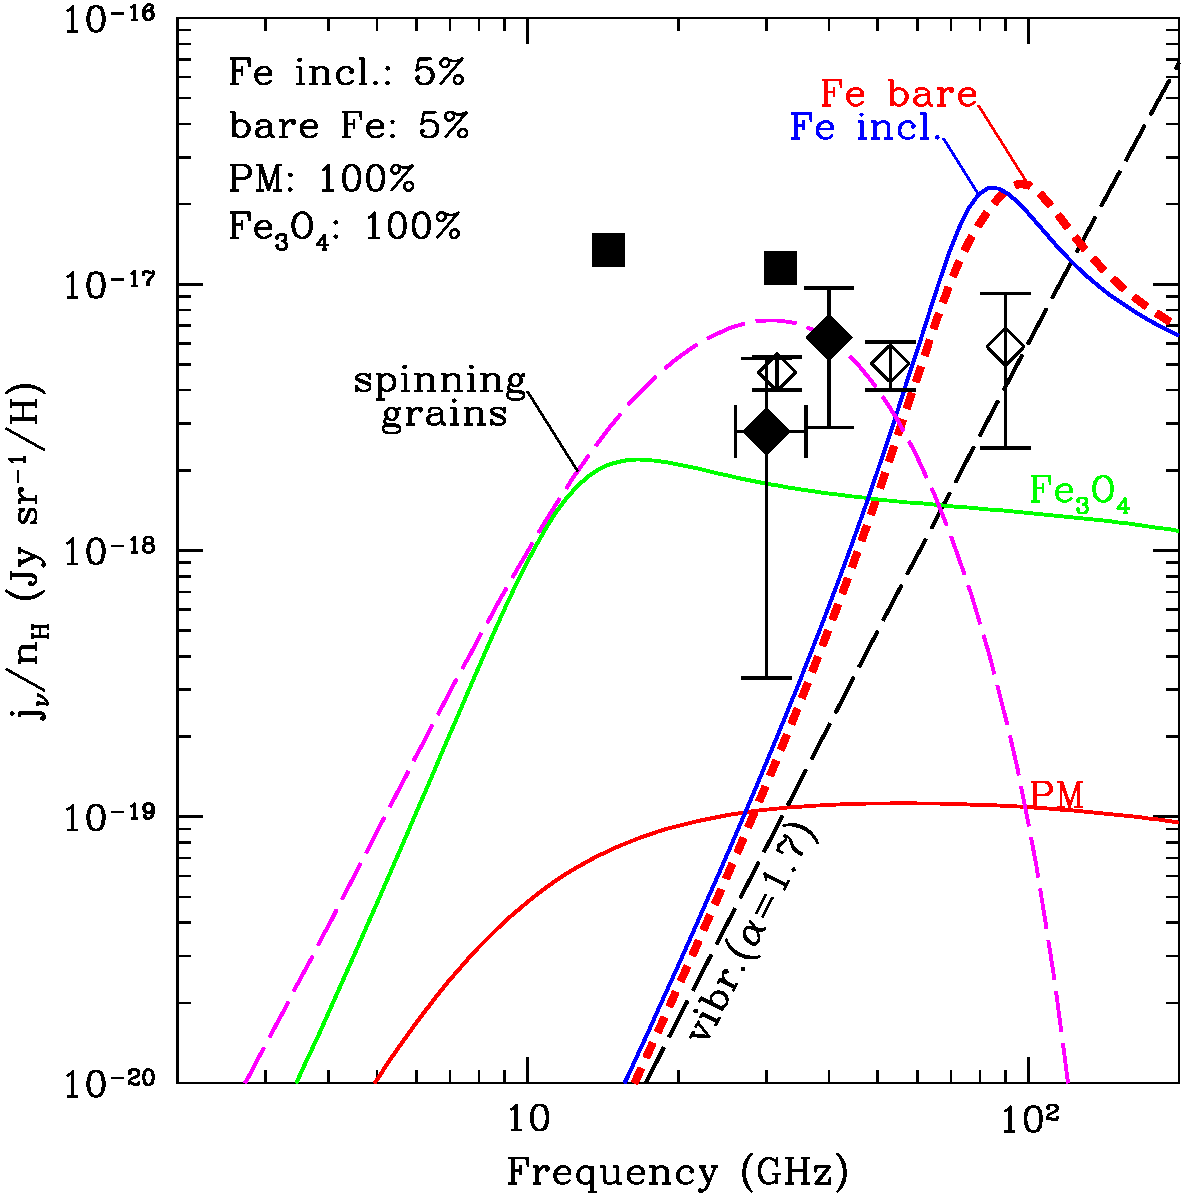
\includegraphics[width=100mm]{EPS/draine99_fig7.pdf}
\caption{From \cite{draine99}, this plot describes an early model of the ''anomalous" modes of dust emission. It is included here to give some perspective on the exptected relative contributions of thermal dust (``vibr., $(\alpha = 1.7)$", long dashed black), spinning dust, and magnetic dust. Squares and diamonds are observational points from early CMB observations. The axes are frequency in GHz (note the peak of spinning dust at ~30~GHz, and how this peak overlaps with all plotted emission components) against intensity per hydrogen column density (Jy $sr^{-1}$/H).They plot the electric dipole (``spinning grains" contribution (magenta long-dashed) along with the various expected magnetic dipole contributions from bulk iron (``Fe bare", short red dashed), grains with iron inclusions (``Fe incl.", blue solid), iron oxides ($Fe_{3}O_{4}$, green solid) and paramagnetic grains (``PM", red solid).} 
\end{center}
\end{figure}
     There a few regions such as $\rho$~Ophiuchi that are still thought to be dominated by spinning dust \cite{casassus08}. Studies of the AME and diffuse galactic emission done by \cite{planckXVii} show some evidence for an additional blackbody microwave component which could be caused by magnetic dust in the diffuse sky.  Whether or not their result also applies to galactic clouds is unclear. \cite{draine99} describes the potential contribution of magnetic dust in the following way: \textit{``one cannot exclude the possibility that magnetic grains make an appreciable contribution to the emission in this frequency range."}

\section{Motivation for Understanding the Anomalous Foreground}
     Perhaps a primary factor for why the AME was ever noticed, and why it is worth understanding, is its interference with non-ISM topics. \cite{leitch97} features a warning to other researchers upon their detection of the AME: \textit{``The detection of such a component suggests that we should be cautious in any assumptions made regarding foregrounds when designing experiments to map the microwave background radiation.”} More recently, it was shown via 
data by \cite{macellari11} that the AME is a dominant component of the microwave foreground at low galactic latitudes. Thus, getting a full picture of the CMB's anisotropies will be difficult without considering the intervening material that is the Milky Way.
     In a similar way, gravitational wave astronomy may be somewhat hindered by the less understood emission mechanisms of interstellar dust. The second-generation of the Background Imaging of Cosmic Extragalactic Polarization observations (BICEP2) reported a detection of a B-mode polarization signal in the CMB in \cite{ade14}.
     Follow up studies have proposed that this initial detection may in fact be confused with the galactic microwave foreground, in the form of magnetic dipole emission from dust \citep{liu14}. However it is still unclear what the contribution from dust could be, as the polarization data is still being reviewed.  In any case, the B-mode polarization due to inflation in the early universe cannot be confirmed without constraining a possible contribution from dust \citep{flauger14,mortonson14}.
     From the ISM perspective too, the AME's origin is important beyond simply its possible confusion with cosmological data. The source of AME has implications for the ISM itself. Spinning dust may be another piece of the ``ISM Interaction Puzzle”. If the AME is linked strongly to spinning dust, or to magnetic dust, it could be used as a probe for ISM conditions.
     Confirmed spinning dust emission could imply possible presence of some certain chemistries (perhaps PAHs, or other small dust having an electric dipole.) For example, confirming that AME = spinning dust, would allow us to probe galactic environments in the case that corresponding vibrational modes of those spinning molecules are found to be missing. If AME is carried by very small dust grains or by PAHs, then microwave emission could be used to trace these molecules more clearly even if their vibrational emission is being obscured along the line of sight. \cite{tibbs14} attempt to derive small grain properties within molecular cores assuming that the AME there is from spinning dust, as an early example of using AME to understand the ISM. 
     Confirmed magnetic dust emission as part of the AME could help to constrain the composition of dust. As \cite{draine99} has shown that grains with Fe inclusions could produce this emission, magnetic dust emission may help determine the abundance of ferromagnetic dust. The search for magnetic dust emission may also be a potential test of the model put forth by \cite{jones14} (see Figure \ref{Jones Dust}) wherein some silicate grains may have iron inclusions.
\clearpage

\section{Contents}  
  In Chapter \ref{chap:Introduction} we have described the basic issues of ISM and dust research, and highlighted the importance of understanding the anomalous microwave emission foreground. The AME is very likely to originate from dust. Spinning dust emission and magnetic dipole emission from dust are the leading explanations.  
  In Chapter \ref{chap:Data} we give an introduction to the data sources used for this work. As this is a study based only on space-telescope data, there are no specific observational techniques to describe. Rather, the relative characteristics of each of the 13 all-sky photometric maps used are discussed. We describe the importance of each instrument, and highlight the advantages of using the new MIR surveys by AKARI/IRC and the newly released  FIR surveys by AKARI/FIS. Most important to this work is the combination of AKARI/IRC and Planck/HFI, and this is shown by the relative response functions of each band.
  The data processing is described in Section 2.4. The major objective of the data processing method is to create a set of maps, ranging the full thermal dust SED, at an identical pixel size and smoothing scale.  We then describe how information regarding the dust at each pixel is inferred, such as the temperature, emissivity index, and relative sub-micron dust abundance. 
  In Chapter ref{chap:Analysis} we describe how the dust properties extracted from the average dust SEDs from each of the AME regions is compared. Plots demonstrate the relative strength of the correlations of each photometric band's average intensity vs the AME amplitude for each ROI. We also update a previous work regarding the ratio of the AKARI/IRC 9~$\mu$m band to the 18~$\mu$m band intensity vs. the significance of spinning dust reported by PCXV.
  In Chapter ref{chap:Discussion} we comment more deeply on the methods used, and discuss possible interpretations of the analysis in Chapter 3. We discuss the lack of strong support for a clear PAH-AME relationship, and present pathways for further investigation.
  A summary is given in Chapter 5.

\chapter{Data
  \label{chap:Data}}
%%% TABLE %%%%%%%%%%%%%%%%%%%%%%%%%%%%%%%%%%%%%%%%%%%%%%%%%%%%%%%%%%%%%%%%%%%%%
\begin{table}[ht]
\label{datasources}
\caption{Observational data sources used in this article}
\centering
\begin{tabular}{lrrrr}
\toprule
Instrument    & Central Wavelength & FWHM~$arcsec$ & Reference  \\
\midrule
AKARI/IRC & 9~$\mu$m     & 5.5$"$	     & \citep{irc07,ishihara10}  \\
AKARI/IRC & 18~$\mu$m	 & 5.7$"$       & \citep{irc07,ishihara10}   \\
AKARI/FIS & 65~$\mu$m    & 32$"$     & \citep{fis07,doi12} \\
AKARI/FIS & 90~$\mu$m    & 30$"$     & \citep{fis07,doi12} \\
AKARI/FIS & 140~$\mu$m	 & 41$"$     & \citep{fis07,doi12} \\
AKARI/FIS & 160~$\mu$m	 & 38$"$     & \citep{fis07,doi12}             \\ 
IRAS/IRIS & 12~$\mu$m    & 3.5$'$          & \citep{iris05}             \\
IRAS/IRIS & 25~$\mu$m    & 3.5$'$          & \citep{iris05}             \\
IRAS/IRIS & 60~$\mu$m    & 3.6$'$          & \citep{iris05}              \\
IRAS/IRIS & 100~$\mu$m   & 4.7$'$          & \citep{iris05}         \\
Planck/HFI & 345~$\mu$m & 4.7$'$ & \citep{hfi14viii} \\
Planck/HFI & 550~$\mu$m & 4.3$'$& \citep{hfi14viii} \\
\bottomrule
\end{tabular}
%\tabnote{}
\end{table}
%%%%%%%%%%%%%%%%%%%%%%%%%%%%%%%%%%%%%%%%%%%%%%%%%%%%%%%%%%%%%%%%%%%%%%%%%%%%%%%
\section{AKARI Space Telescope}
     The AKARI (Astro-F) infrared space telescope revealed an entire sky of infrared light, at wavelengths from the mid to far infrared, via two instruments \citep{akari07} the Infrared Camera (IRC)\citep{irc07} and the Far Infrared Surveyor (FIS)\citep{fis07}. Six all-sky maps were created, allowing for exploration into a great expanse of interstellar environments. The infrared sky had never before been revealed with such fine resolution at nearly unconstrained spatial coverage. In this work and many others, AKARI data has illuminated many patterns in the Milky Way. AKARI gave us a wealth of pointed imaging and spectroscopy observations, though for this study we have focused on the all-sky maps at 9, 18, 65, 90, 140, and 160~$\mu$m.

\subsection{AKARI/Infrared Camera}
     The Infrared Camera instrument on-board AKARI was designed to study the near to mid-infrared range, and was thus enabled with 7 observable wavebands. The world's only all-sky PAH-band survey, the IRC's 9~$\mu$m all-sky map demonstrates the abundance of the PAH bands carrier in the Milky Way \citep{ishihara10}. It is true that other instruments are capable of collecting emission from the PAH bands. However there is no other photometric instrument which has such a complete coverage of all of the major bands, at 6.2, 7.7, 8.6, and 11.2~$\mu$m \citep{onaka99,irc07}. In fact, the only other photometric survey with all-sky coverage at the MIR, the IRAS 12~$\mu$m band, did not collect any light from the 6.2, 7.7, or 8.6~$\mu$m bands, though it was somewhat sensitive to the 11.2~$\mu$m. WISE/Band 3 also has full-sky coverage, though its response functions are very similar to IRAS/12~$\mu$m. The Spitzer/IRAC bands are the only other photometric survey which dense coverage of the PAH bands. Though the wavelength coverage, sensitivity, and resolution of Spitzer/IRAC are extremely useful, the pixels are simply not available for most of the sky. Therefore, for the type of large spatial range study featured in this thesis, there is no other instrument suitable to investigate the PAH features than IRC. 
\begin{figure}[htbp]
\begin{center}
\label{allbands}
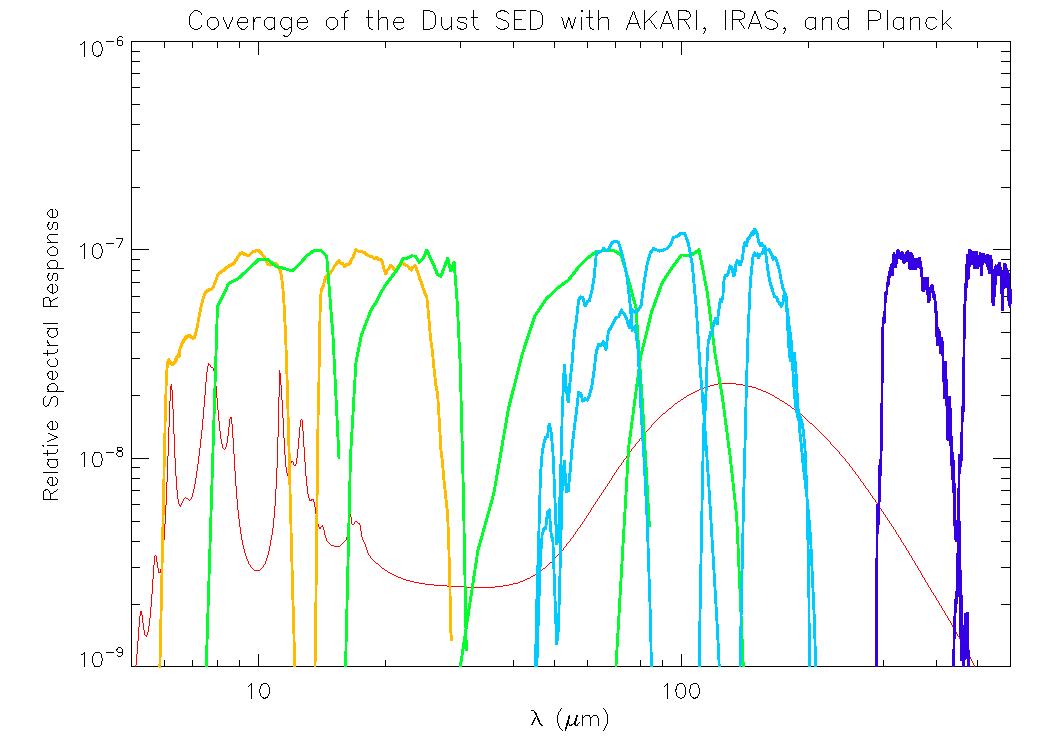
\includegraphics[width=150mm]{EPS/AKARI_rsr_thesis.pdf}
\caption{This figure describes our multi-wavelength analysis of the full vibrational dust SED.  The y-axis gives arbitrary relative response units. The x-axis shows the covered wavelength range in microns.The filter of each instrument's survey used in this study is plotted along with a sample dust mixture model SED computed by DustEM \citep{dustem11}. The AKARI/IRC 9 and 18~$\mu$m bands are shown in orange, FIS bands in turquoise, IRAS bands in green, and the Planck/HFI bands in purple. Most importantly, note the complete coverage of the major PAH/UIR bands 6.2, 7.7, and 8.6~$\mu$m by IRC \cite{ishihara10}. The IRAS 12~$\mu$m band's coverage starts at about 8~$\mu$m. The peak of the thermal emission curve is well covered by FIS.  The FIR tail of the thermal equilibrium emission curve is constrained by HFI.  To clarify, there is no significant contribution from AME at these wavelengths. These data are not intended to measure AME directly; only the corresponding information from thermal dust emission from AME regions is gathered.
 }
\end{center}
\end{figure}
%%%Let's put the filter response curves here
\begin{figure}[htbp]
\begin{center}
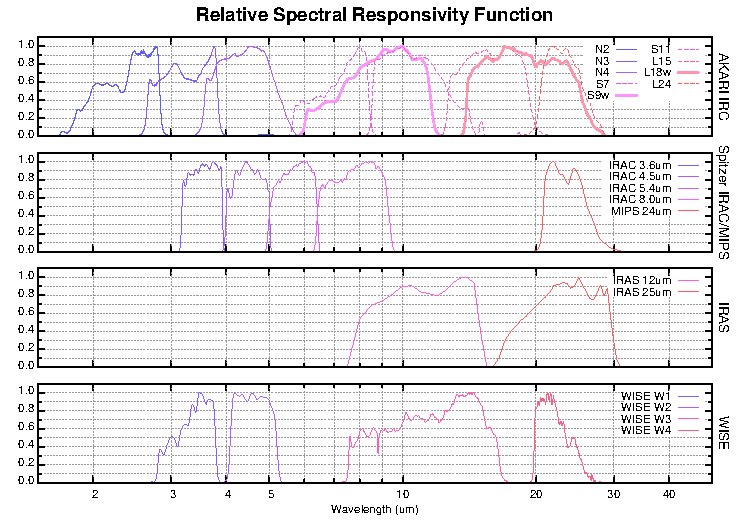
\includegraphics[width=150mm]{EPS/rsr.pdf}
\caption{
This image shows the filter response curves for the AKARI IRC bands vs. the bands from comparable instruments on-board the Spitzer, IRAS, and WISE infrared space telescopes. The most important thing to note is the coverage of the AKARI IRC 9~$\mu$m band vs. that of the IRAS~$\mu$m band and (and WISE band 3 which is very similar). The PAH / UIR bands cut-off just short of the IRAS 12~$\mu$m bands coverage, whereas the AKARI 9~$\mu$m survey spans most of the PAH bands, and the flux it observes is expected to be dominated by them. Though their central wavelengths are similar, we expect that the IRAS 12~$\mu$m and AKARI 9~$\mu$m bands contain very different information about the dust SED. While the Spitzer 8~$\mu$m band is similar, There is no other survey with such complete spectral and spatial coverage of the PAH bands. AKARI is a critical tool for this type of PAH investigation spanning such a large number of ROIs.
 }
\label{rsr}
\end{center}
\end{figure}
\subsection{AKARI/Far Infrared Surveyor}
     The Far Infrared Surveyor (FIS) gives us photometric data around the peak of the typical dust SED. FIS was equipped with four wavebands: two narrow bands centered at 65~$\mu$m and at 160~$\mu$m, and two wide bands at 90~$\mu$m and at 140~$\mu$m. An all-sky scanning survey was carried out at each band \citep{doi12}, and the processed maps have been recently released at the time of this writing. Figure \ref{fig:FIS} shows the all-sky map at 140~$\mu$m produced by FIS.
%%%\citep{doi14}%%%%
\begin{figure}[!htb]
\begin{center}
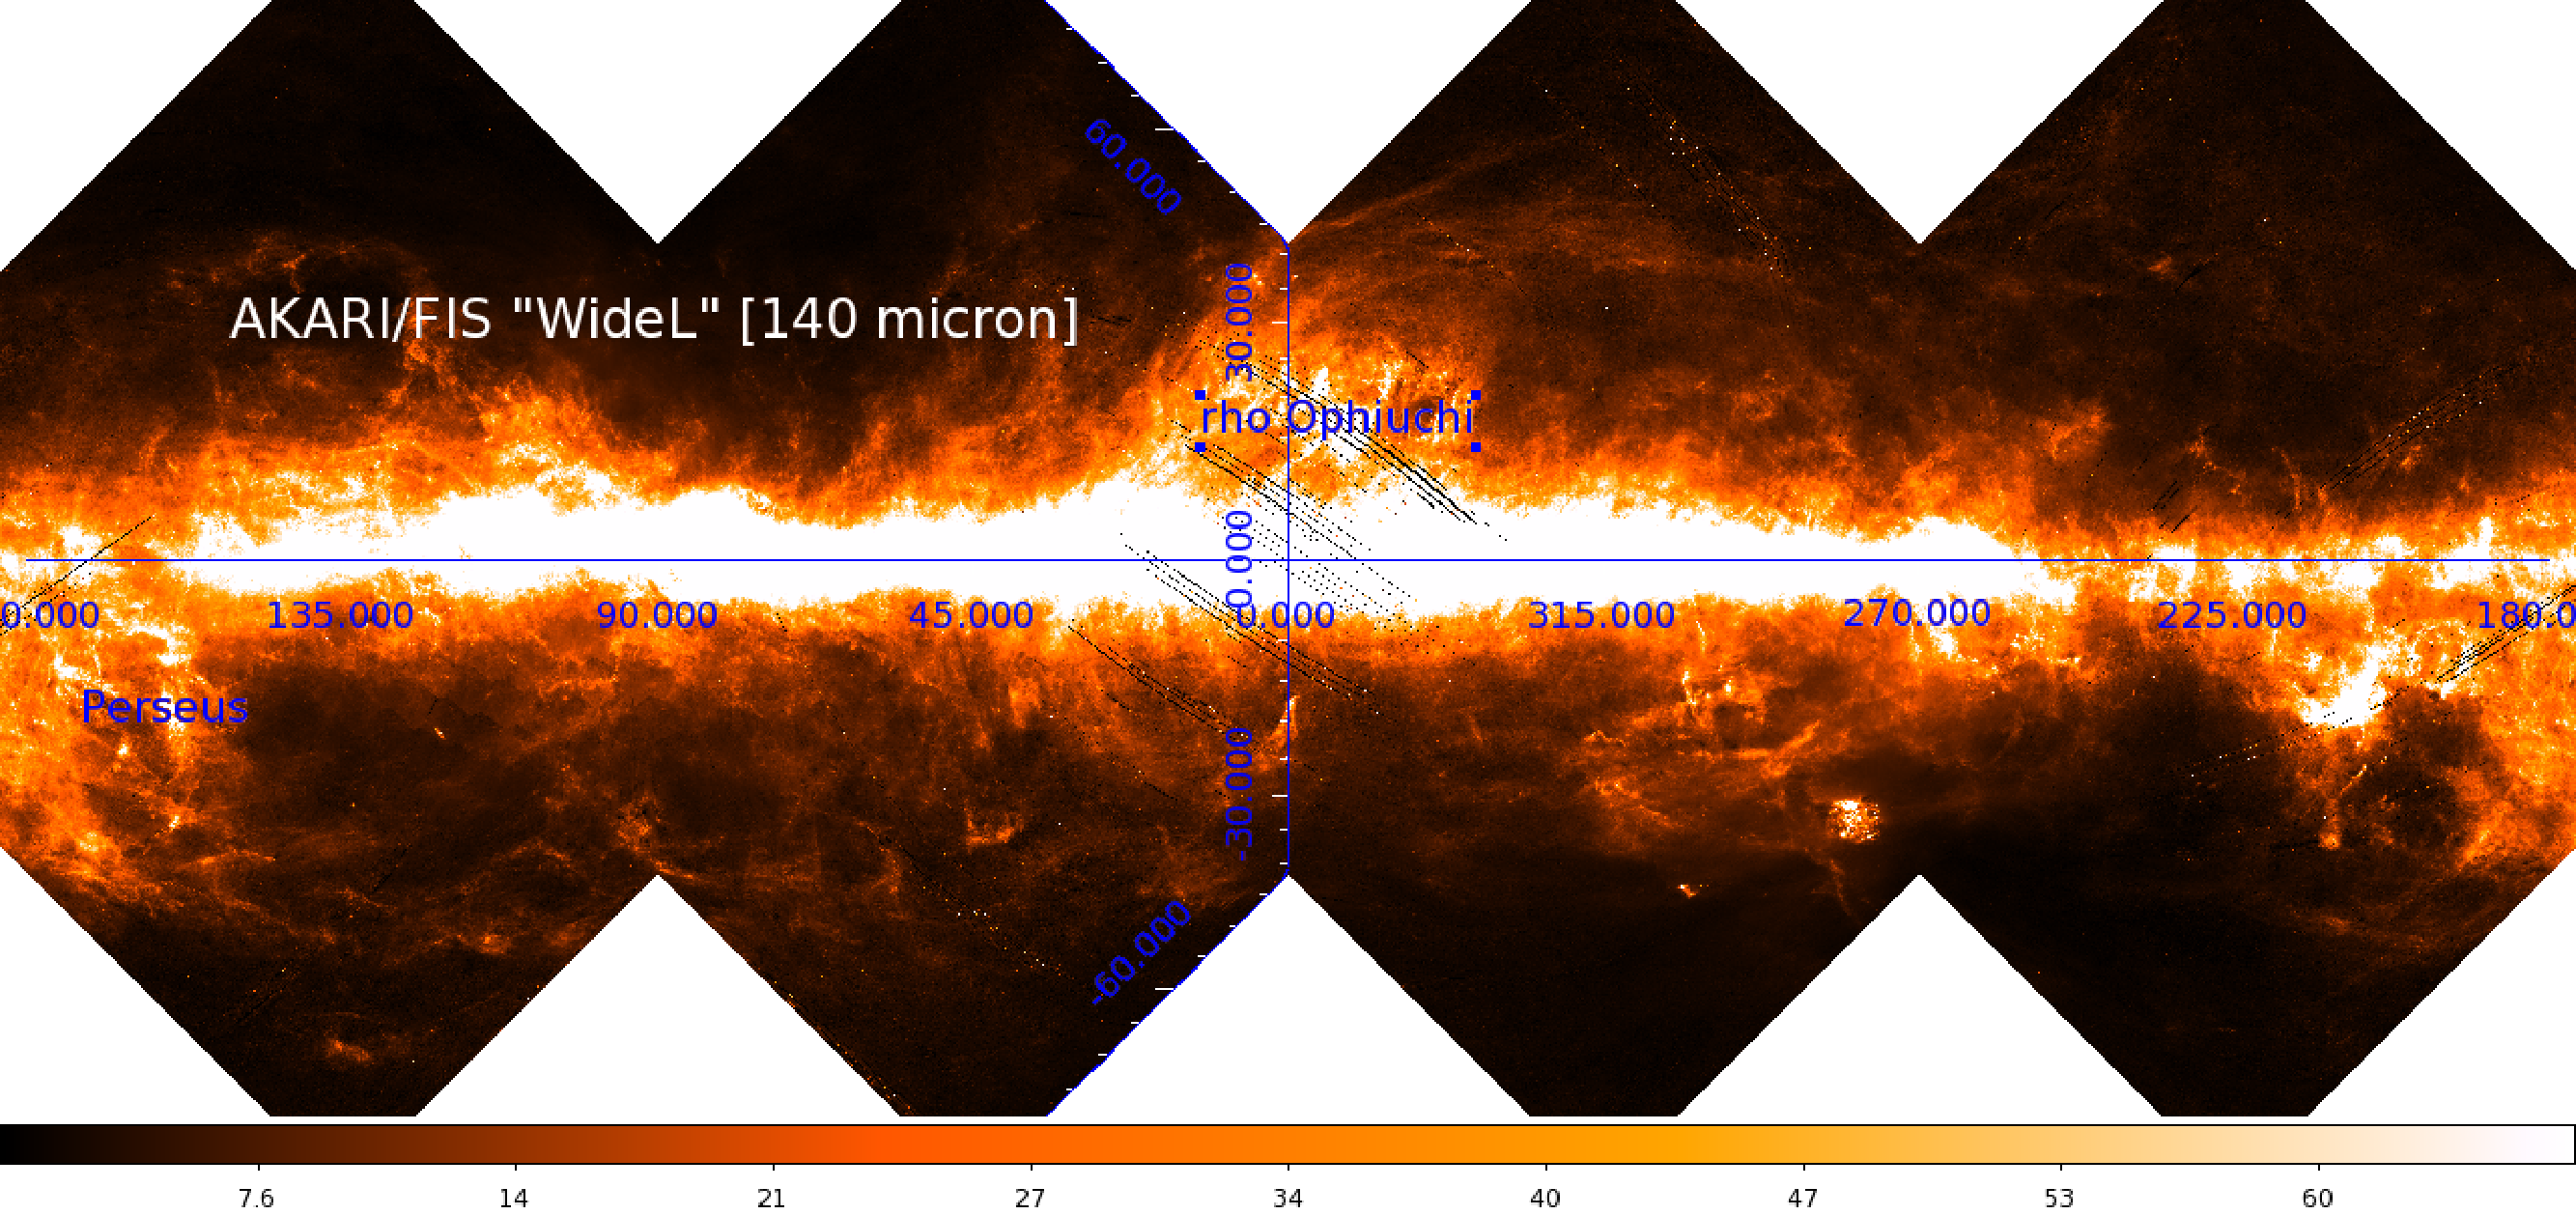
\includegraphics[width=170mm]{EPS/im_akari140.pdf}
\caption{This is the Milky Way according to the AKARI/FIS 140~$\mu$m data. The two most prominent AME regions, Perseus and $\rho$~Ophiuchi are labelled in blue. The coordinates are Galactic. This is the highest resolution data available in the FIR wavelengths, with such wide spatial coverage. The stripe errors which affect mostly the regions around Ophiuchi are visible. This map is the HEALPix 1.7arcmin/pixel version (much lower resolution than the $~$30~arcsec original all-sky maps). The colorbar is in MJy/sr.}
\label{fig:FIS}
\end{center}
\end{figure}



The narrow bands have a higher noise-level compared to the wide bands. However the absolute photometric uncertainty per pixel has yet to be evaluated. The main point is that FIS samples a critical part of the dust SED not sampled by IRAS, and at galactic latitudes beyond the reach of the Spitzer Space Telescope \citep{spitzer04}.

\section{Planck High Frequency Instrument (HFI)}
     The latest and most accurate CMB surveys are created by the Planck Space Observatory (Planck), with its Low Frequency Instrument (LFI)  ranging from 30 to 70~GHz \citep{lfi14ii}, tracing the peak CMB and a large portion of the galactic foreground, and its High Frequency Instrument (HFI) spanning 100 to 857~GHz \citep{hfi14viii}, which traces much of the galaxy’s thermal emission.
     While the largest-scale patterns of the sky, those of the CMB have been studied carefully by both the LFI and HFI, the HFI instrument has talent for ISM research as well. The far infrared thermal emission tail of the dust spectral energy distribution can be constrained by the HFI’s photometric bands. This study uses the all surveys in the 857~GHz (345~$\mu$m) and 545~GHz (550~$\mu$m) bands, respectively, for their unique coverage of the post-peak dust SED complemented the SED-peak constraints provided by AKARI/FIS. These data points are critical for regions-of-interest that were spatially beyond the reach of Planck’s partner sister observatory, Herschel. Without Planck data we cannot strongly constrain the temperature and column density of interstellar dust.
\section{IRAS}
     Data from the Infrared Astronomical Satellite \citep{iras84} all-sky surveys are used to supplement the similarly-centred AKARI photometric bands. Including IRAS data offers a more dense sampling of the dust SED in regions where Spitzer or Herschel data are simply non-existent.T
     The IRAS 12~$\mu$m band is similar to the AKARI 9~$\mu$m band in terms of the sky coverage, central wavelength, and especially in that both surveys are heavily dominated by zodiacal light. The model of zodiacal dust emission (zody) by \cite{mrr13} utilized for the Improved Reprocessing of the IRAS Surveys (IRIS) \citep{iris05} is an important benchmark for the zody-subtraction from the AKARI/IRC surveys.
\section{All-sky Data Handling}
\subsection{Data Extraction}
       The data extraction process uses primarily standard routines, relying on the Interactive Data Language (IDL) platform. The framework for the data processing outlined below essentially follows the structure prepared by Fr\'ed\'eric Galliano for the Herschel-Planck School 2013 (http://ecole-doctorale.obspm.fr/-Program-). The course utilized example IDL routines and Herschel data as a curriculum to teach basic processing and dust SED fitting of an extended object. In this study, those examples are adapted and expanded to handle AKARI data. A color-correction step is added which is based on the DustEM IDL wrapper code \citep{dustem11}. The final step of Galliano’s example is to apply a custom full dust SED fitting routine. However dust model templates for this step have not yet been created for the AKARI data. The average SEDs for each region are instead piped to the DustEM code. The results between DustEM and Galliano’s model will be compared in a future work.
\subsection{Target Selection}
%%%***Include Table***%%%
     Regions of interest (ROI) were chosen based on their relevance to AME research. In general, we follow the work of PCXV. In this recent study of the AME in the dense galactic ISM, candidate “spinning dust regions” were selected using a 2 to 3 degree wide selection criteria. 2 degree-wide apertures which showed excess emission after subtraction of synchrotron, free-free, CMB, and thermal dust emission, were listed as candidates. The Planck team then conducted a multi-wavelength SED modelling of each region at all Planck/LFI and HFI frequencies, to determine the likelihood that its excess is explained by spinning dust. For this purpose they employed the ``SPDUST” model, developed by \cite{ali-hamoud09}. Some targets were shown to be extremely likely spinning-dust regions, such as $\rho$ Ophiuchi with a confidence level of $~30\sigma$. Other regions were dismissed as spinning dust targets by PCXV after spectral modelling, as in the case of the Orion Nebula whose SED was well explained by free-free emission. \par    
     The original intention of this thesis was to look at the fine-scale spatial variations of the dust SED, primarily at the MIR wavelengths relevant to PAHs/very small dust, in $\rho$ Ophiuchi and Perseus. We intended to compare works such as \cite{tibbs11} which focused on Spitzer data, with data from AKARI. This is why we first do a pixel-by-pixel analysis of each ROI. However the strategy was modified later on when the PCXV results were released, identifying a large number of candidate AME regions. We now focus on the average SED of each ROI for the purpose of understanding the AME. This method may also be generally useful as a study of the typical AKARI+IRAS+HFI SED across a large number of galactic clouds.
     This thesis first aims to complement the PCXV analysis of AME regions by contributing dust SED analysis using unique compilation of photometric data, i.e. the AKARI/IRC 9~$\mu$m survey’s coverage of the PAH/UIR bands. We have selected ROIs having an array of AME significance values. Regions such as Orion, described as “non spinning dust regions” in PCXV are used as a control against regions suspected to exhibit spinning dust.

\subsection{HEALPiX maps}
     In the case of the FIS, HFI, and IRAS bands, ROI’s are cut-out out from all-sky .FITS files, structured according to the Hierarchical Equal Area isoLatitude Pixelization (HEALPix) scheme \citep{healpix05}, a standard data format conceived to handle very large data sets, and originally used for the WISE surveys. It works very efficiently as a framework for all-sky maps processing, especially in the case of degrading to a lower pixel resolution. There are also many standard routines available for processing HEALPix-formatted data. 
     In this work, the particular advantage that ROI cut-outs can be very easily created from a pre-compiled HEALPix array was desired. The ROIs are extracted using a “cookie-cutter” routine with the very recallable name of GNOMDRIZZ, part of the publicly available DRIZZLIB IDL package.  Cut-outs for each of the FIS, HFI, and IRAS bands are extracted easily, without the need to mosaic a series of tile images.  The HEALPix framework also defines common resolution tiers, and the “Resolution Level 11”, or NSIDE 2048 is chosen for the processing described here. This is the highest common resolution map offered across the three instruments, having a pixel scale of 1.7$'$. During the GNOMDRIZZ extraction, we keep the 1.7$'$ pixel scale for the tangential projection of each map according to the galactic coordinate system. We believe the 1.7$'$ pixel scale is in good proportion to the 857~GHz band’s beam-size of 4.7$'$.
\subsection{Region extraction}
     In order to keep a standard reproducible method for our data processing, all of the ROIs are handled in the same way. The NSIDE 2048 native pixel scale of 1.7$'$ is kept, and a pixel dimension of 47 is chosen so that each ROI cut-out is (80$')^2$ . Given the typical size of the primary ROI class (HII regions falling in an ``AME zone", usually around 0.5\degree wide), an 80$'$ square map should be appropriately sized to contain both the ROI and a sufficient number of background pixels. Figure \ref{fig:PCXVresmap} shows the residual map from PCXV from which their AME ROIs were selected.
\begin{figure}[htb!]
\begin{center}
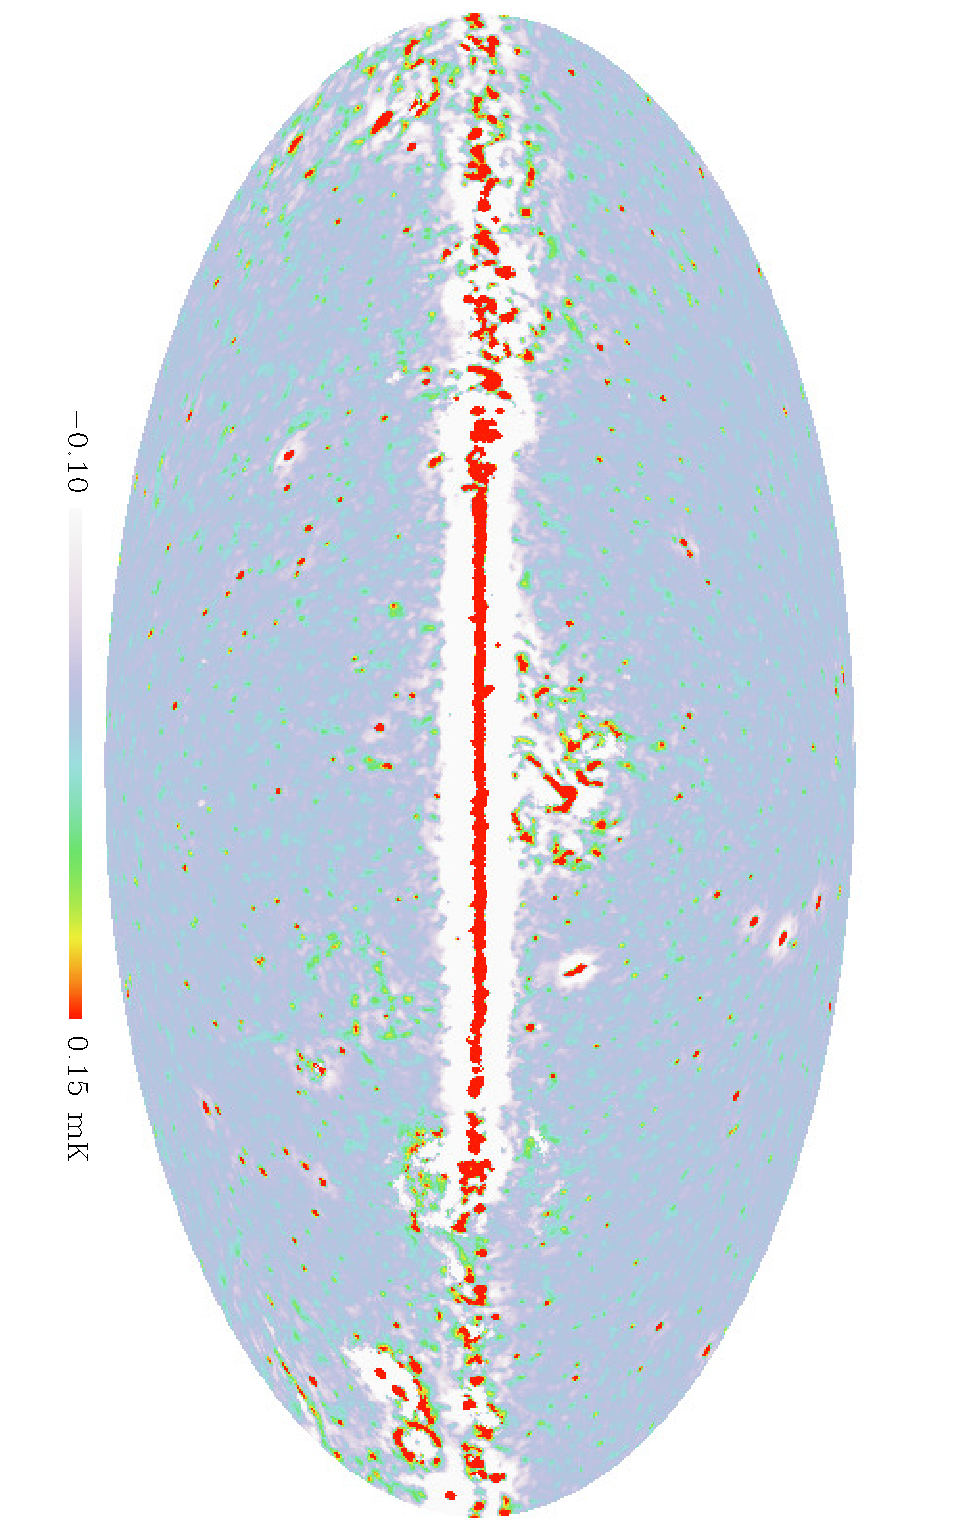
\includegraphics[width=80mm, angle=90]{EPS/planckXV_fig1.pdf}
\label{PCXVmap}
\caption{This map illuminates the suspected AME regions across the entire sky. From \cite{planckXV}, the authors subtracted models of free-free, synchrotron, and thermal dust emission from the LFI 28.4~GHz map to produce this ``residual map" which is a general tracer of  the AME. Many of the bright red regions in this image are believed to exhibit spinning dust emission.}
\label{fig:PCXVresmap}
\end{center}
\end{figure}

\subsection{Background Subtraction}
     Background subtraction is always an interesting problem and especially for these types of near-by ISM complexes having non-trivial structures. The possibility of subtracting the target emission itself along with the ``background” is a common risk. For very bright regions where the only significant source of background emission is the zody, we believe that a simple flat background subtraction is suitable. A fitted-plane background subtraction may be appropriate for regions near to the ecliptic plane, such as $\rho$ Ophiuchi. For other, faint regions, or those within the galactic plane where chances of confusion with other targets is higher, a more careful approach is ultimately desired. In the case of FIS data, the smooth component of the zody has already been subtracted. The IRAS/IRIS data has already been zody-subtracted. 
     In this first study however, we have adopted a standard way to subtract the background. We subtract a flat-average background from each ROI using a commonly available routine ``BACKSUB”, in the Buie Astronomy IDL Library.Other background methods may be more or less effective, depending on the region, however we have chosen to keep a very standard procedure for this study. Later studies will utilize a more sophisticated subtraction approach, and compare the results for various methods (i.e. flat-mean subtraction vs. 2D polynomial subtraction.
     Following the background-subtraction, the arrays for each region are ``zoomed-in”. We decrease the image size to include only a 30~$'$ square patch around the ROI’s center coordinates. This width is chosen as a suitable average size range for each region. A larger window leaves us over-sampling background positions for some narrower ROIs, while a smaller window may be offset from the cloud’s structure. In the PCXV analysis which we initially followed, a 1$\degree$-radius circular aperture was used for sampling. However their maps were also subject to a much coarser smoothing, using a 1$\degree$ Gaussian beam. Our study is not directly comparing infrared data to the low resolution microwave data, thus this smoothing is not needed. However in a later analysis, we would like compare our present study with the same analysis done according to the PCXV smoothing and aperture size.
\subsection{Pixel masking}
%%Insert a figure showing the masking of the saturated pixels of Orion %%%
     Upon the final SED extracting and modified blackbody fitting, any pixel which is masked at any of the sampled wavebands, is masked for the entire fitting. The final mask is a super-position of all of the individual wavebands’ masks. In other words, only pixels which are unmasked for all wavebands are used. 
     Pixels having negative values after the background subtraction are masked from the analysis. In this way, we are assuming that those pixels were too close to the ``true background level”. Rather than adjusting the background level to avoid negative values, we mask these pixels from the data processing and SED fitting. 
     Due do this super-positioning of masks, the background mask size and shape is more sensitive to the IRC data. This is because there is a tendency for the bright regions in the AKARI/IRC data to be more compact than the same regions as observed by AKARI/FIS. Thus the final sampled portion of each ROI is biased towards the apparent region size seen in the AKARI 9 and 18~$\mu$m all-sky data.          
     Pixels that already have zero or ``not-a-number” values applied to them during the original data reduction remain masked in this study. They are not filled in with data from alternate surveys. In any case, this masking is not a common issue; usually it is a result of saturated pixels covering very bright targets. The center of Orion (M42) is a good example, in the FIS data. $\rho$~Ophiuchi contains some missing ``stripes” due to the AKARI’s pointing being changed to accommodate individual observation requests during the all-sky scanning of that region. Neither of these issues (over-saturation or missing stripes) have been relevant for the Planck HFI data. 
\subsection{Resolution Degrading}
     All of the data in this analysis was smoothed according to a larger beam size, because of one disadvantage incorporating the Planck HFI data. The beam size of the 545~GHz band is roughly 4.7$'$. This means the native resolution AKARI data is not comparable to the Planck data, or IRIS data, in a pixel-by-pixel manner. Despite the disadvantage, Planck’s extended FIR wavelength coverage is critical to make a trustable SED fitting. In order to find a compromise, we degrade the resolution of AKARI IRC and FIS data to that of the Planck HFI beam. While it is perhaps superficially discouraging to degrade visually appealing high resolution data, in this case the SED coverage is of a higher priority. Even HFI’s larger beam size is fine enough for our purposes this type of large-scale study.
     All of our data is convolved with the largest beam of the Planck HFI 545~GHz waveband, having a resolution of about 4.7$’$. The beam’s shape is sufficiently elliptical that we have acquired the publicly available Planck Legacy Archive HEALPix file containing the HFI-team-provided PSF, rather than simply convolving with a circular Gaussian beam. This allows us to at least keep the resolution of our final data set at 4.7$’$. As we were initially interested in smaller-scale variations (before expanding the number of ROIs to include all 98 PCXV regions). We felt that convolving with a larger artificial circular Gaussian PSF would have unnecessarily constrained our study. For future work we may experiment with a much coarser smoothing. 
     We are interested not only in the average SED of each ROI, but also, as much as possible, we want to begin to understand the structural variations within the region. The actual convolution processing is handled by the IDL routine \textit{DO\_THE\_CONVOLUTION} which is publicly available and developed by \cite{aniano11}.
     We have not created kernels between the AKARI data and the Planck data, nor between the AKARI/IRC and AKARI/FIS.  The Planck beam is sufficiently large compared to the respective beam sizes of the AKARI instruments that a kernel was not needed. For future purposes, it will be useful to create convolution kernels between the IRC and FIS beams, such that we can explore the structural detail in these surveys side by side.
\subsection{Regridding}
     A ``regridding” step is included so that the positions of the cut-outs made from HEALPix maps (as in the case of AKARI FIS) can be aligned with cut-outs which are made via mosaicking the original survey tiles (as in the case of AKARI IRC). All of the HEALPix maps are already aligned to the same grid during the drizzling process, which creates a rectangular FITS file from a HEALPix map. At that time a galactic World Coordinate System (WCS) and identical pixel scale and image dimensions are chosen. However images not created using the HEALPix standard routines need to be re-gridded so that they match, pixel-by-pixel, the positions of the HEALPix-generated cut-outs.
\subsection{Color Correction and Modified Blackbody Fitting}
     One fundamental issue in photometric studies is that such bandpasses are not evenly sensitive at all wavelengths which they cover. Therefore, there is some deviation between the emission which they observe and what is actually being produced. We may never be able to infer perfectly what the actual source's emission characteristics are. Fortunately, we can get a good approximation of the sources SED if we first know what type of emission it is most likely producing. Then we may use the observed emission to scale a template SED model. In the case of thermal dust emission in the FIR, we expect the continuum emission to basically take the shape of a blackbody, though with a correction applied to the emissivity. The form of the equation for such emission was given in Chapter 1:
\begin{equation*}
\tag{1.3.3}
I_d(\nu) \propto \nu{}^{\beta{}_d}B_\nu{}(T_d)
\end{equation*}
     We first fit the non-color-corrected data with the above equation, fitting $T$ to each one (with $\beta$ fixed at 2.0), as well as an ``amplitude" (explained more carefully in Chapter 3). With this initial fitted model spectra, we convolve with response functions of the bands greater than 65~$\mu$m to obtain the color correction factors. The color-correction routine is borrowed from the DustEM IDL wrapper code \citep{dustem11,dustem13}.
     The color correction factors are then applied to the observed intensities of their corresponding bands. Finally, the modified blackbody fitting is run again in order to obtain the $T$ and amplitude of the expected FIR SED at each unmasked pixel.
     Using the fitted values, a mean average of the temperature, and the color-corrected intensity at each wavelength, is taken across the unmasked pixels. These average values, calculated for each of the 98 ROIs from PCXV are used in the plots against AME parameters (from the same paper) in Chapter 3.
%\subsection{Black-hole Sample Return Mission Results}
%Unfortunately the entire mission apparatus (including the human components) was spaghettified exactly as predicted. However we have no way of knowing if this really happened or not, as no information was retrieved from the event. There was one slight anomalous increase in the X-ray flux from the AGN for a moment of time that we cannot quantify. We can only conclude that science is a lot of fun, and we would gladly do it all over again.
%\section{High Resolution Case Study: Perseus and $\rho$ Ophiuchi}
%In addition to the large scale data extracted across all regions presented in PCXV, we examined two very heavily studied AME candidates: the Perseus Molecular Cloud Complex and $\rho$ Ophiuchi. We examine these two regions spatially in the IRC 9 and 18~$\mu$m data at their native resolution vs. contours derived from the Planck 2014 Release "low-frequency diffuse emission" map.

\chapter{Analysis}
     Here we present several comparisons of the data processed according to Chapter 2 vs. the AME properties determined in PCXV.  We describe an estimation of the FIR-emitting dust optical depth abundance vs. the spinning dust amplitude $A_{sp}$. From PCXV, $A_{sp}$ is \textit{``essentially the flux density at the peak normalized to the spinning dust model."}.  We also include a look at each waveband's averaged intensity described in Chapter 2, for each of the 98 ROIs, vs. the $A_{sp}$. This band-by-band fitting is repeated with the average intensities scaled by interstellar radiation field strength (ISRF) of each ROI (the ISRF is given as $G0$, which is the ISRF strength compared to that of the solar neighborhood). Lastly, we revisit an earlier result of the 9 to 18~$\mu$m ratio vs. the significance of the spinning dust model fit for each ROI. Our previous result included only 10 ROIs from PCXV, the present result includes all 98.

\section{Dust Optical Depth vs. AME Amplitude}
     After color-correction and obtaining a fitted value the temperature, $T$ and optical depth at 250~$\mu$m, $\tau_{250}$. of each pixel, we estimate the relative total far infrared emission (FIR) at each pixel using the following equation, where $\lambda$ is the wavelength in microns, $\tau_{250}$ is the optical depth at 250~$\mu$m, and $B(T)$ is the Planck function:

\begin{equation}
\label{FIR}
FIR = \tau_{250\mu m} \int_{0}^{\infty} [250\mu m/\lambda(\mu m)]^{\beta}
B_{\lambda}(T) d\lambda ,\;
%\label{totalFIR}
\end{equation}
%To explain further, we must carefully introduce a conventional term, "sub-micron dust". This term does not cover all of the dust which is smaller than one micron. PAH carriers and VSGs are not included in "sub-micron dust". Instead, this term refers to grains which are large enough to emit in a classical way (modified blackbody), but are not larger than one micron. 
     The total FIR emission derived above is a result of the incident radiation on the dust (essentially, the incoming starlight) and the column density of the FIR-emitting dust. This property of dust emission is well-described in \cite{onaka00}. For our analysis we use $\tau_{250\mu m}$ as a tracer of the FIR-emitting, or ``classically emitting" dust, This is because $\tau_{250\mu m}$ is proportional to the column density of FIR-emitting dust; FIR emission at 250~$\mu m$ should be dominated by the modified blackbody emission from such grains. The FIR emission does not include very small grains or PAH-type molecules. 
     For the present analysis, we use a version of the modified blackbody fitting where $\beta$ is fixed at 2. The issue of the most appropriate treatment of $\beta$ will be revisited in a future investigation, where we allow beta to vary.
     The above calculation is carried out for each of the 98 candidate regions, and plotted against $A_{sp}$. Figures 3.1 and 3.2 show resulting plot for the regions with high AME significance and regions of low AME significance, respectively. While our comparisons with the PCXV AME parameters uses only the averaged results of the modified blackbody fitting, we have included the pixel-by-pixel results as well in Appendix A. There you can see each region's structure in terms of $T$, $\tau_{250}$, $G0$, and reduced $\chi^2$. Appendix B shows the average SED plots of each region: the averaged observed intensity at each waveband overplotted with the region's average modified blackbody curve.

%We also show the results using a slightly different comparison. Instead of $A_{sp}$, we use the ``residual flux" of each ROI in the 28.4 GHz Planck LFI band. Since we have not done our own modelling of the spinning dust spectrum, we felt it is best to include also a more robust comparison with the AME. A comparison of the IR bands with the residual 28.4 GHz flux is independent of a spinning dust explanation. However in order to compare them directly, we first convert our data to flux density units by multiplying by the solid angle of each region. The solid angle is obtained from the count of the unmasked pixels for each ROI, multiplied by the solid angle per pixel. One potential issue however is that in order to determine the AME flux density, thermal dust must be subtracted. The Planck Collaboration subtraction of thermal dust from the LFI data is based on the HFI data. If this subtraction is not complete (i.e. the residual AME flux is not entirely residual), it may complicate the situation since we are attempting to compare the thermal dust information vs. the AME.
     
\subsection{Non-Significant AME Regions}
     To investigate if there is a difference in the correlation of sub-micron dust relative abundance in regions well-modelled by a spinning dust spectrum vs. those that are not, we separate the ROIs into two subsamples. Figure 3.2 shows that there is still a correlation with $A_{sp}$ for the low AME significance regions ($\sigma AME < 5$). However the correlation is slightly weaker than with the regions that are fitted nicely by the spinning dust model ($\sigma AME > 5$).      
\begin{figure}[!htbp]
\begin{center}
\label{fig:tauvsaspnosp}
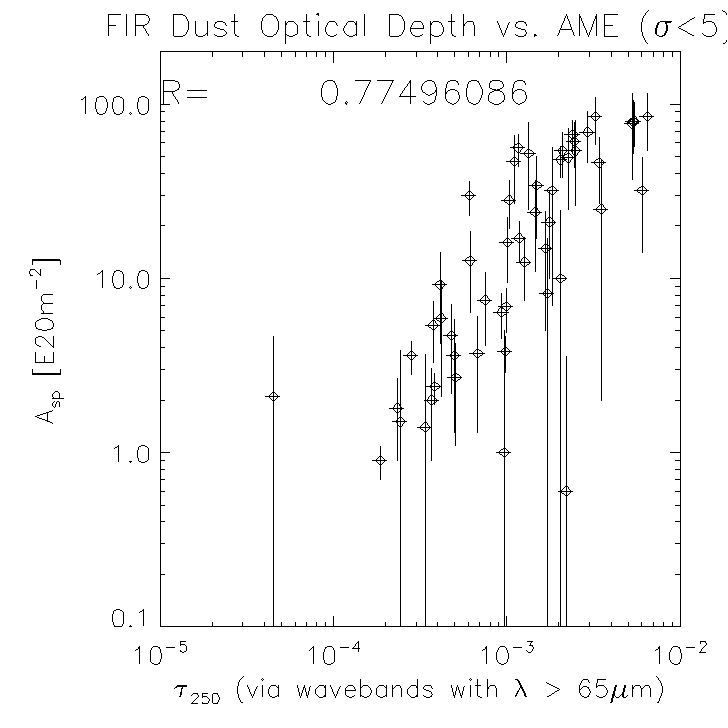
\includegraphics[width=150mm]{EPS/tau250vsAspnosp_masterpres.pdf}
  \caption{ This figure shows only the regions having an AME significance below 5$\sigma$. The correlation coefficient R is 0.77. These regions are classified as ``non-significant AME regions" in \cite{planckXV}. The error bars here are larger by definition, since $\sigma AME$ is given by PCXV as the S/N ratio of $A_{sp}$.}
\label{sub-micron dust vs. Spinning dust}
\end{center}
\end{figure}

\subsection{AME Regions}
     Finally, regions that PCXV found to be well-fitted by the spinning dust model are plotted as a subsample (see Figure \ref{fig:tauvsaspsp}). These regions all have a $\sigma$AME value $>$ 5. The subsample size is smaller than that of the non-significant AME regions (Figure 3.1). Again we can note a correlation, and that it is marginally stronger than the correlation using non-significant AME regions. We expect the correlation in Figure 3.2 to be the stronger one, assuming dust carries the AME.
\begin{figure}[!htbp]
\begin{center}
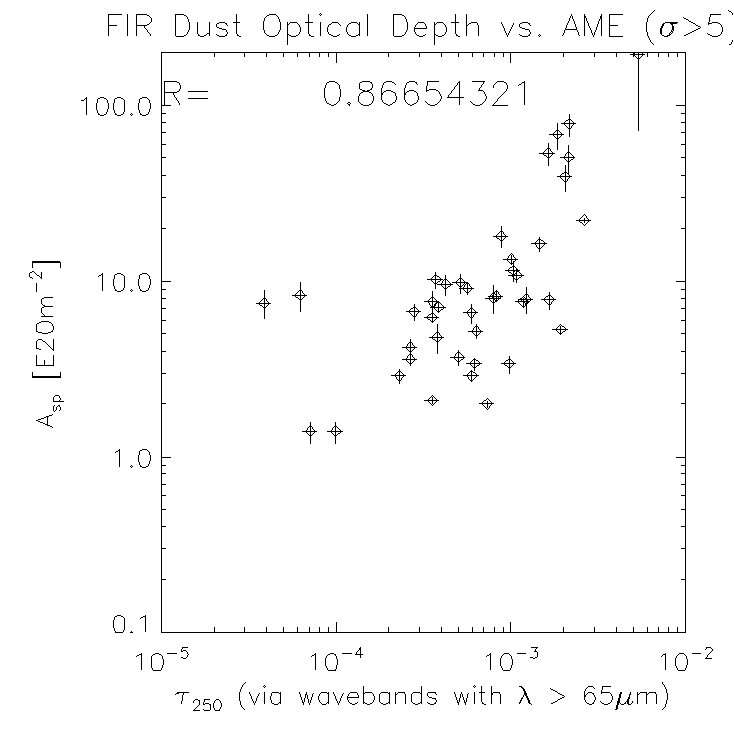
\includegraphics[width=150mm]{EPS/tau250vsAspsp_masterpres.pdf}
  \caption{The counterpart to Figure 3.1, this plot shows $A_{sp}$ vs. the relative sub-micron dust abundance for significant AME regions. The correlation coefficient R is 0.87. These regions have $\sigma$ AME $\>$ 5. This plot shows a slightly stronger trend than the plot of non-significant AME regions}
\label{fig:tauvsaspsp}
\end{center}
\end{figure}     
     
\section{Band-by-band Comparison against AME Amplitude}
     We perform a simple comparison of the averaged IR intensity vs. the spinning dust amplitude (PCXV) of each of the 98 ROIs. Our objective is to explore the possibility of a link between specific dust populations, such as PAHs, and the AME. As described in the introduction, such efforts have already been made by PCXV, \cite{leitch98}, and \cite{ysard10a} with respect to the IRAS all-sky maps. Looking at the individual bands' photometry, especially at the MIR bands, is important because MIR emission which seems in excess of the sub-micron dust abundance is thought to trace very small grains (VSG) or PAHs. 
     We present for the first time an AME vs. IR comparison via AKARI/IRC and FIS in Figures \ref{fig:IRIntMWAmpsp} and \ref{fig:IRIntMWAmpnosp}. These are shown along with the previously investigated IRAS bands. Additionally, we have utilized the HFI bands at 857~GHz and 545~GHz in order to constrain the long wavelength tail of the FIR thermal emission. We compare the relative strengths of the correlations across all 13 bands. As further analysis, Figures \ref{fig:IRIntG0MWAmpsp} and \ref{fig:IRIntG0MWAmpnosp} show how the results change when the IR intensity is scaled by the ISRF strength, $G0$.

\subsection{Average Infrared Intensity $I({\lambda})$ vs. AME Amplitude $A_{sp}$}
Figure \ref{fig:IRIntMWAmpsp} shows each waveband's averaged intensity for each ROI against the AME amplitude, $A_{sp}$, of each region. At least a weak covariance is seen for all bands.

\begin{figure}[!htb]
\centering
 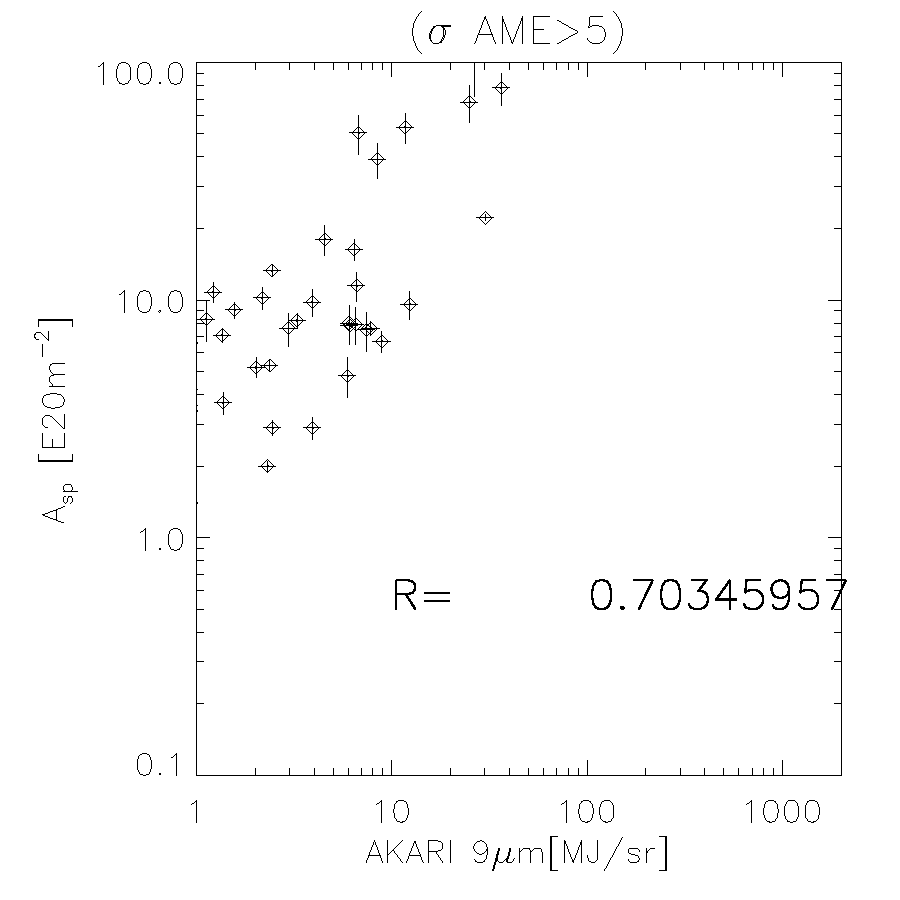
\includegraphics[width=50mm]{IRIntMWAmp/akari9_Asp_sp.pdf}
  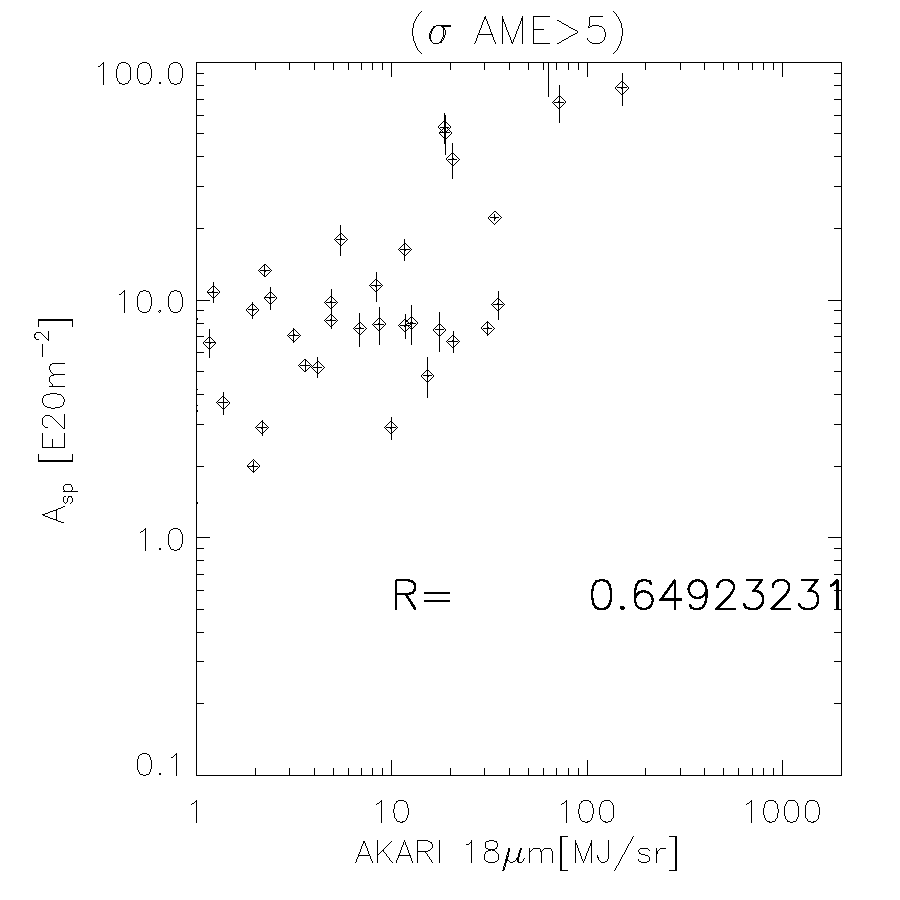
\includegraphics[width=50mm]{IRIntMWAmp/akari18_Asp_sp.pdf}
  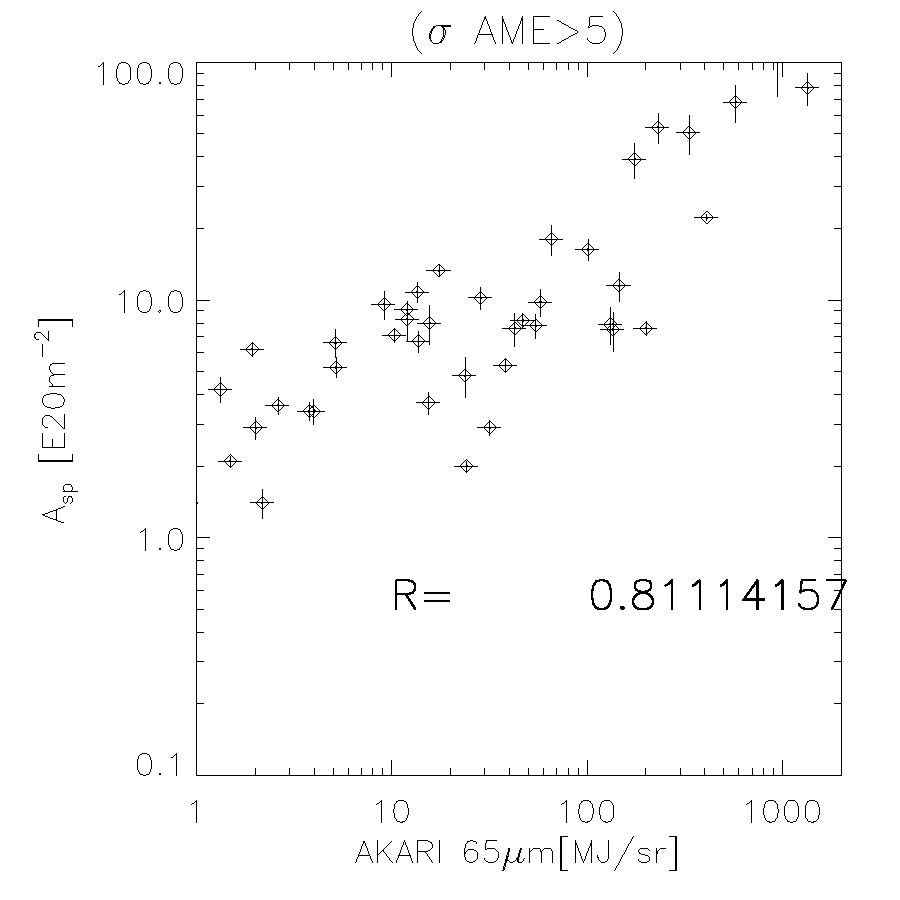
\includegraphics[width=50mm]{IRIntMWAmp/akari65_Asp_sp.pdf}
  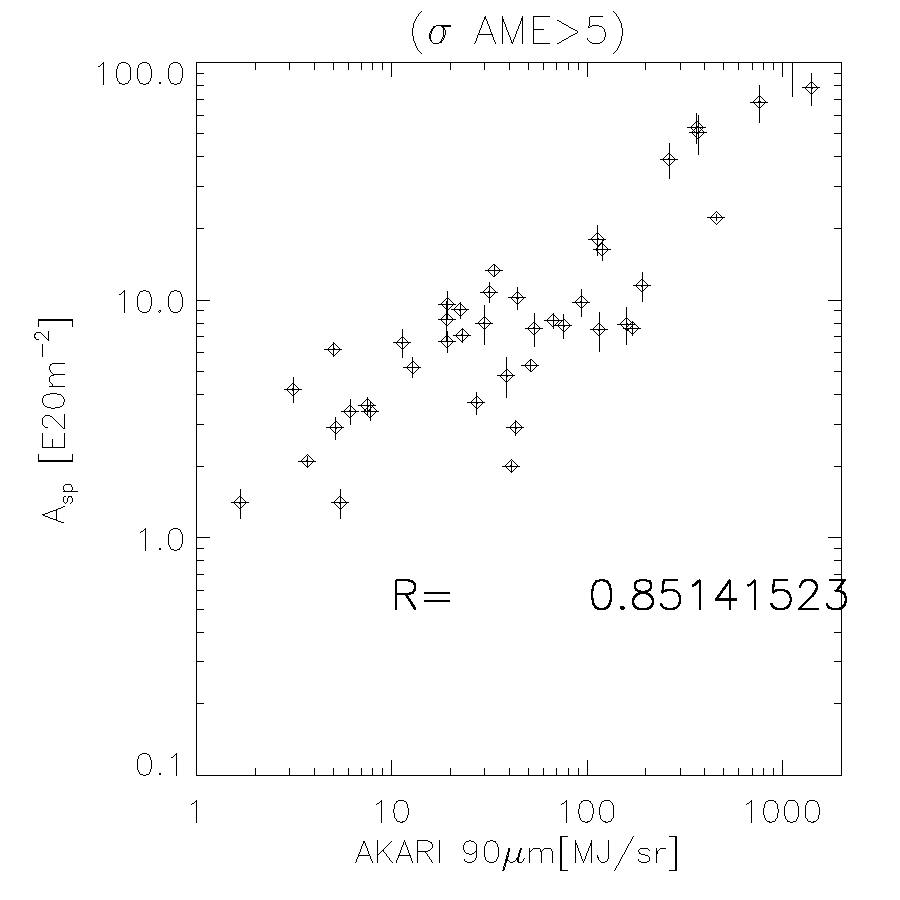
\includegraphics[width=50mm]{IRIntMWAmp/akari90_Asp_sp.pdf}
  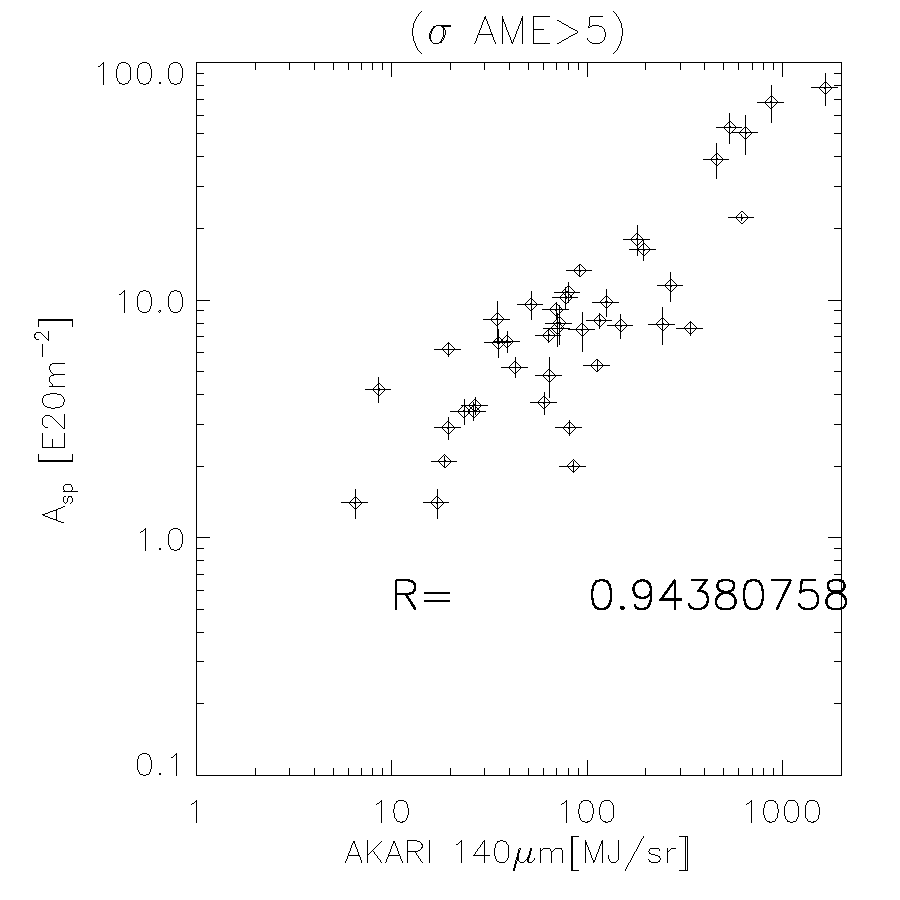
\includegraphics[width=50mm]{IRIntMWAmp/akari140_Asp_sp.pdf}
  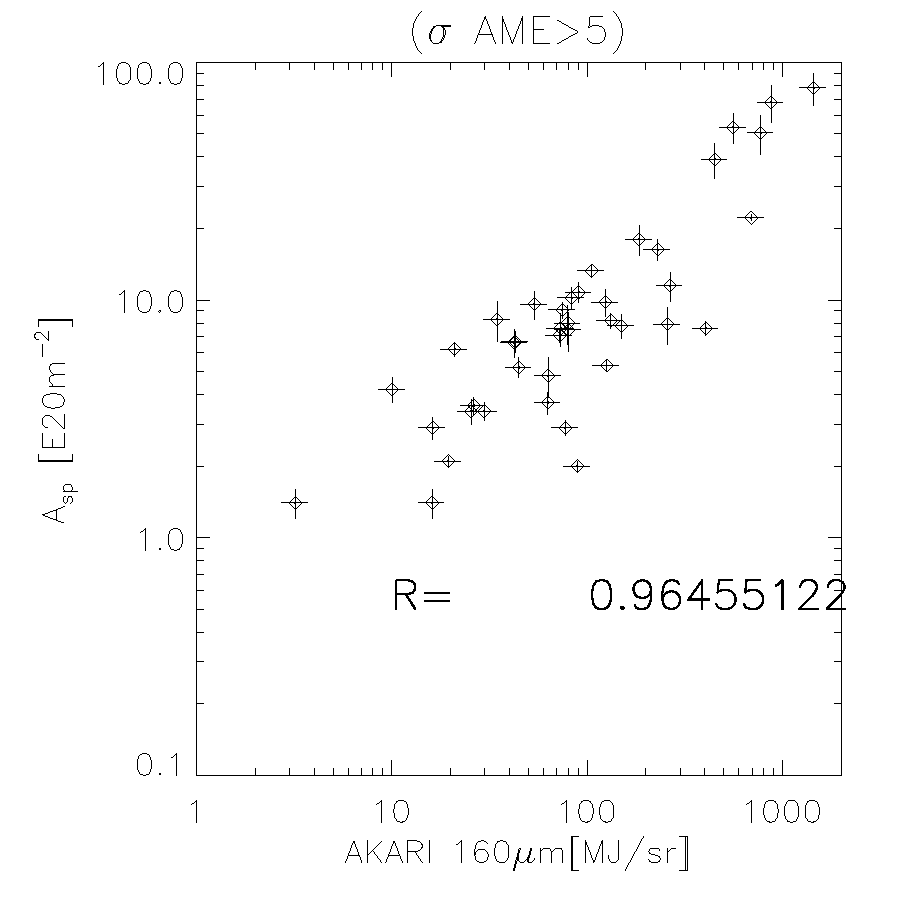
\includegraphics[width=50mm]{IRIntMWAmp/akari160_Asp_sp.pdf}
  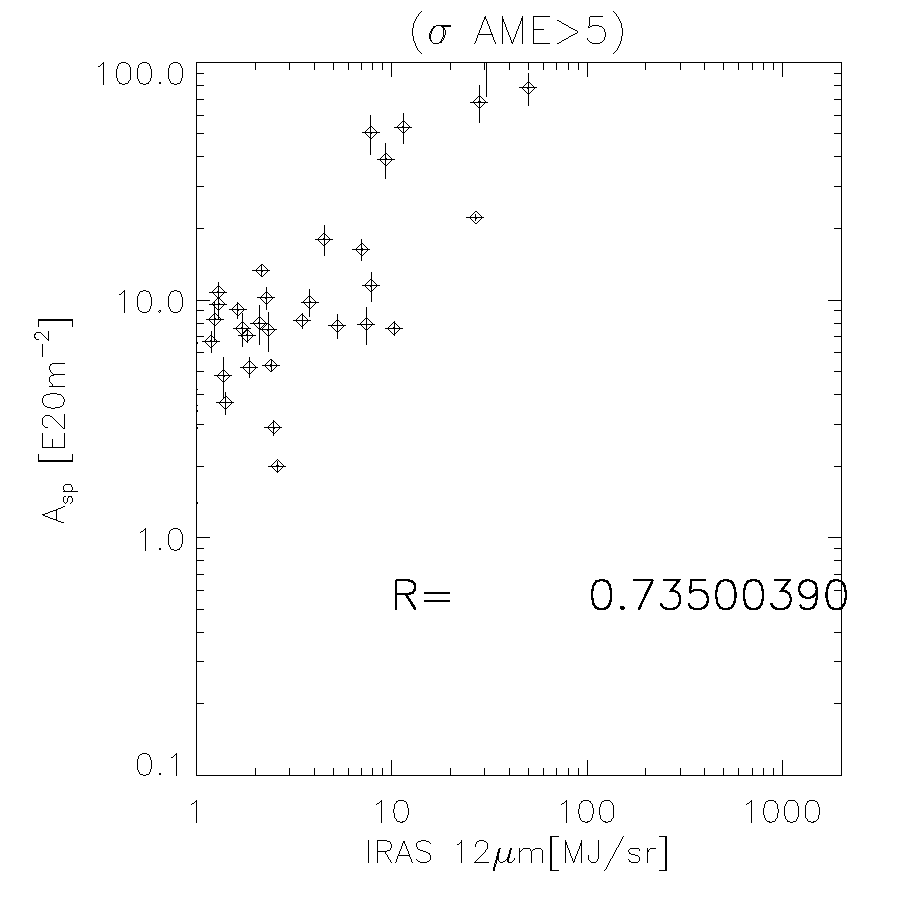
\includegraphics[width=50mm]{IRIntMWAmp/iras12_Asp_sp.pdf}
  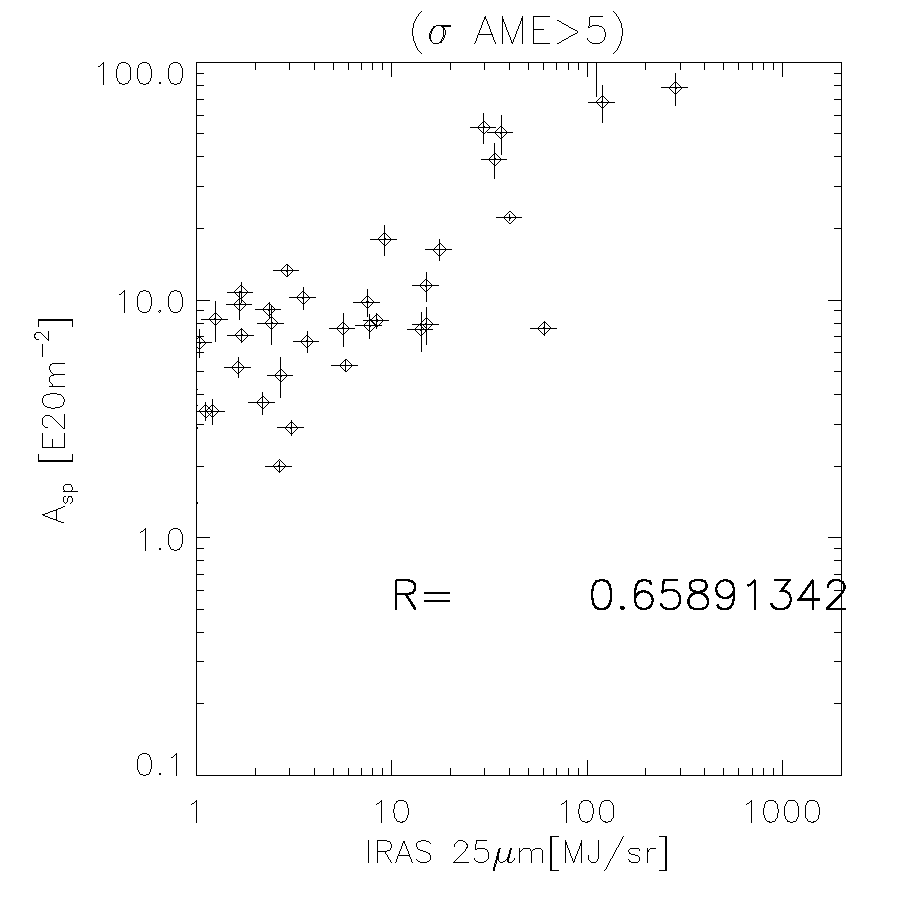
\includegraphics[width=50mm]{IRIntMWAmp/iras25_Asp_sp.pdf}
  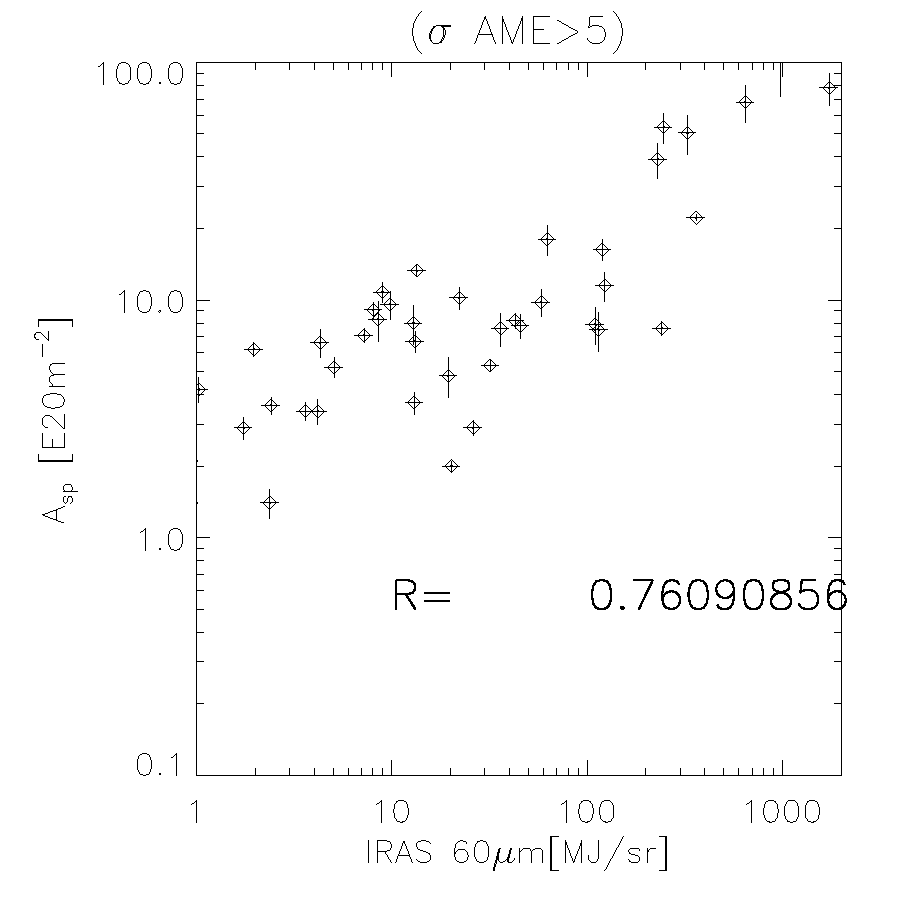
\includegraphics[width=50mm]{IRIntMWAmp/iras60_Asp_sp.pdf}
  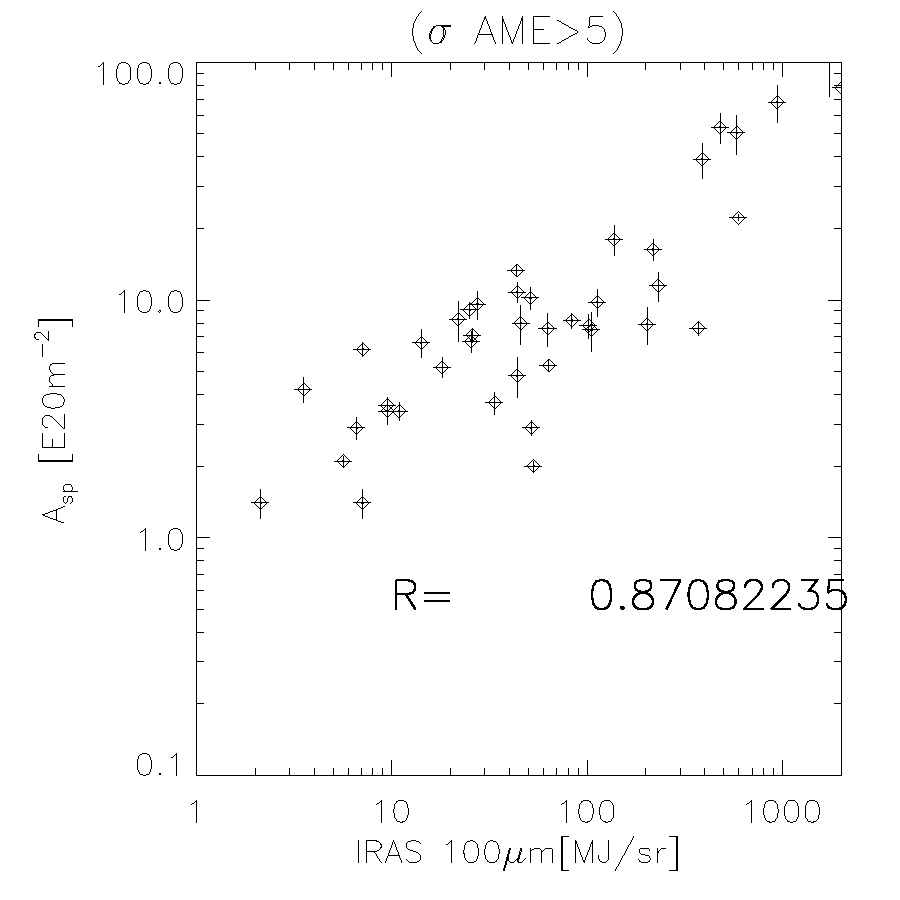
\includegraphics[width=50mm]{IRIntMWAmp/iras100_Asp_sp.pdf}
  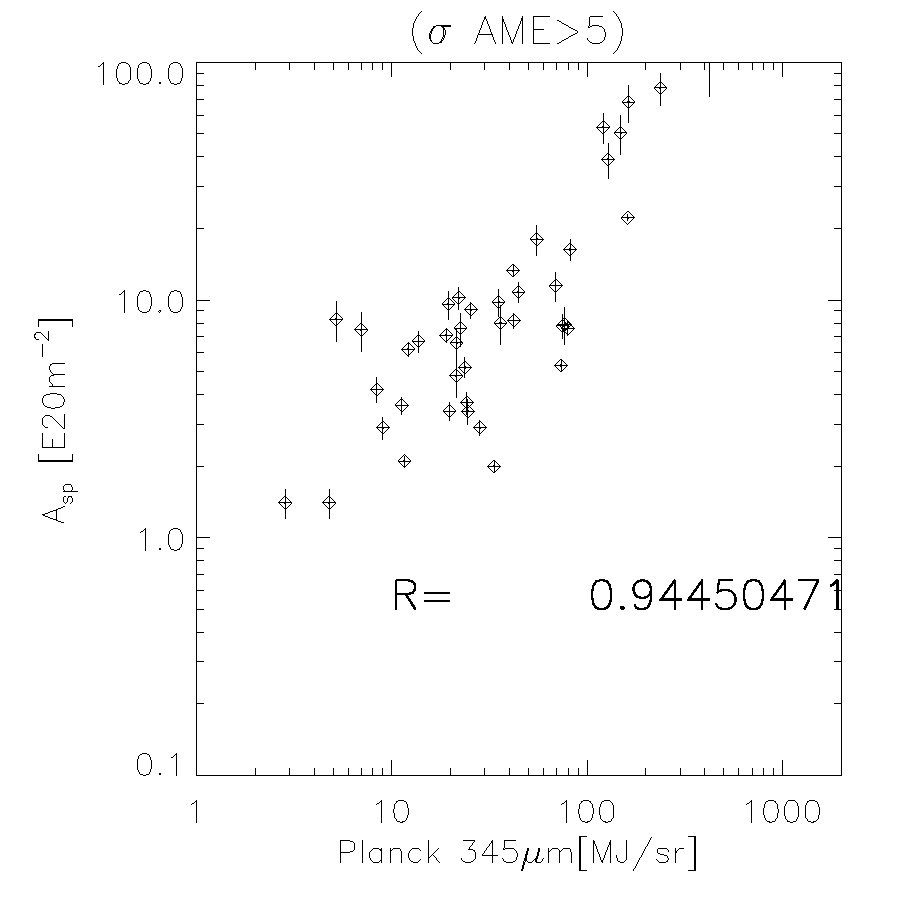
\includegraphics[width=50mm]{IRIntMWAmp/planck857_Asp_sp.pdf}
  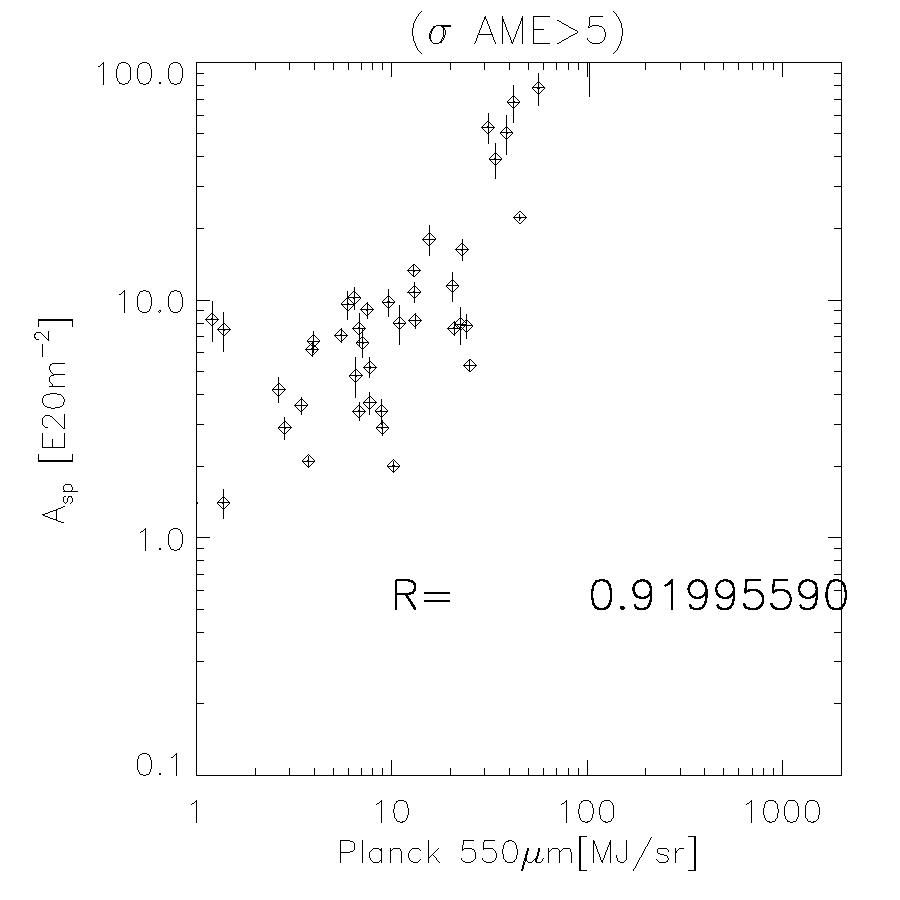
\includegraphics[width=50mm]{IRIntMWAmp/planck545_Asp_sp.pdf}
\caption{AME Amplitude vs. Infrared Photometry: Shown above for each waveband used in the analysis (from AKARI/IRC 9~$\mu$m to Planck/HFI 550~$\mu$m) are the average infrared intensities of each AME region from PCXV against each region's $A_{sp}$ value. These figures are roughly comparable to Figures \ref{planckcorrel} and \ref{ysardcorrel} from \cite{planckXV} and \cite{ysard10a}, respectively. A tighter fit to the AKARI 9~$\mu$m and other MIR bands (stochastically emitting dust) vs. that of $\tau_{250}$ (classically emitting dust), is not seen.
}
\label{fig:IRIntMWAmpsp}
\end{figure}
\begin{figure}[!htb]
\centering
 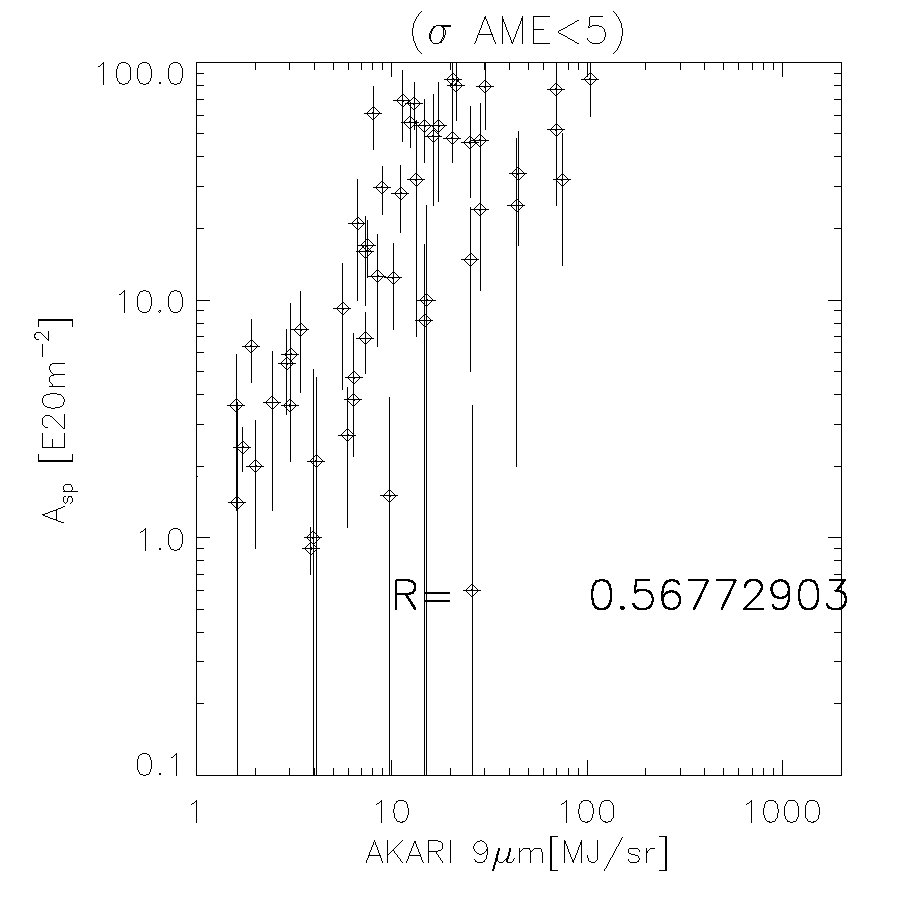
\includegraphics[width=50mm]{IRIntMWAmp/akari9_Asp_nosp.pdf}
  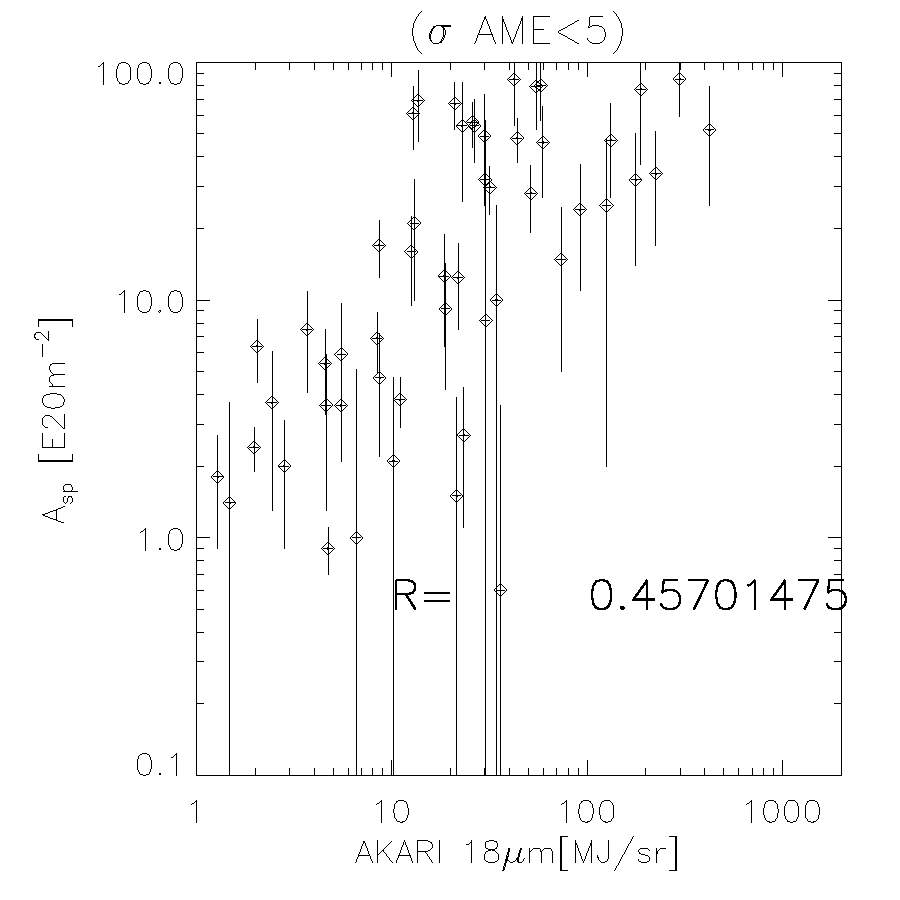
\includegraphics[width=50mm]{IRIntMWAmp/akari18_Asp_nosp.pdf}
  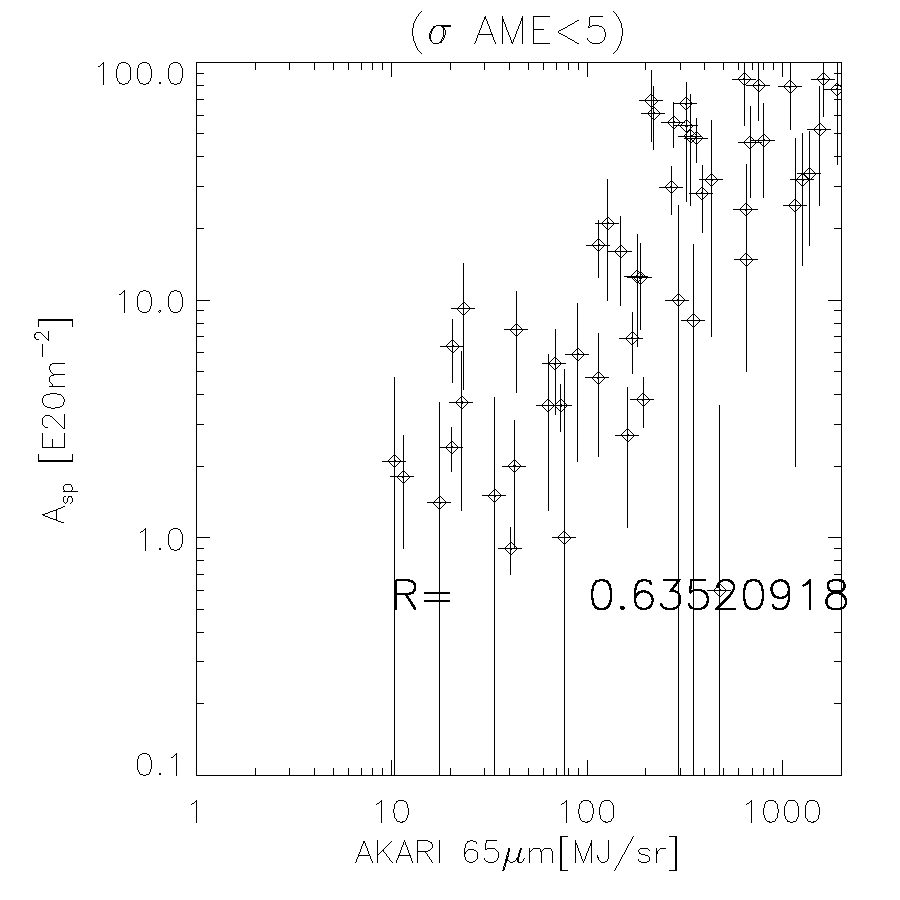
\includegraphics[width=50mm]{IRIntMWAmp/akari65_Asp_nosp.pdf}
  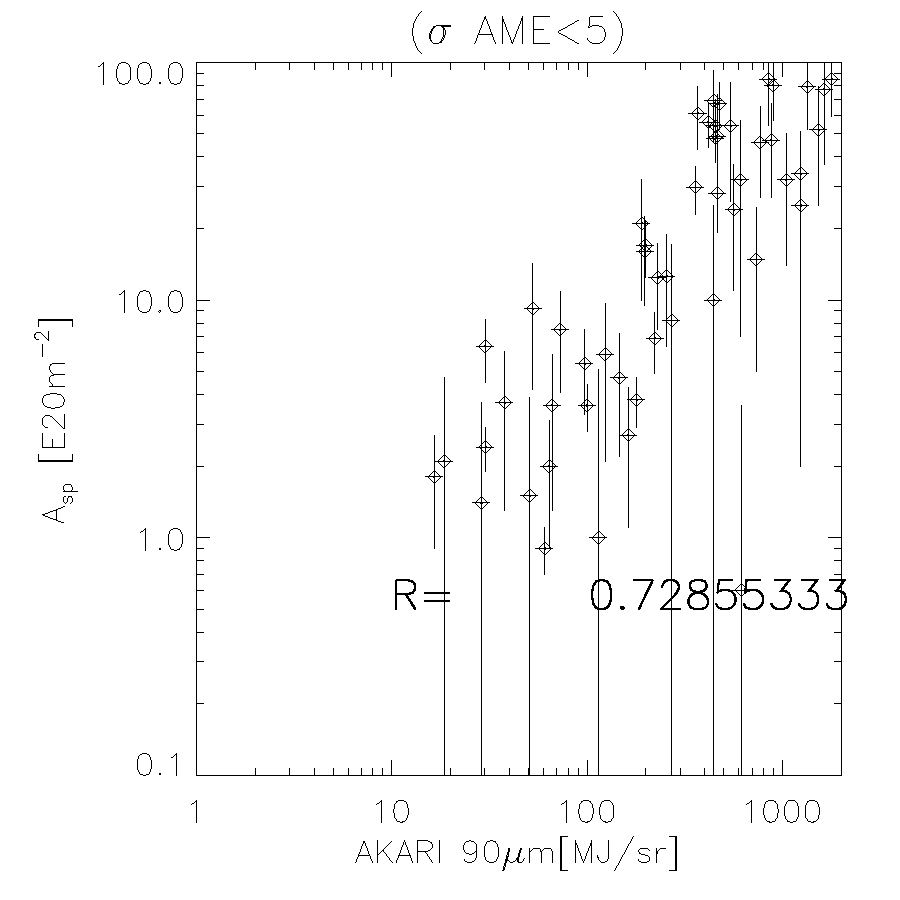
\includegraphics[width=50mm]{IRIntMWAmp/akari90_Asp_nosp.pdf}
  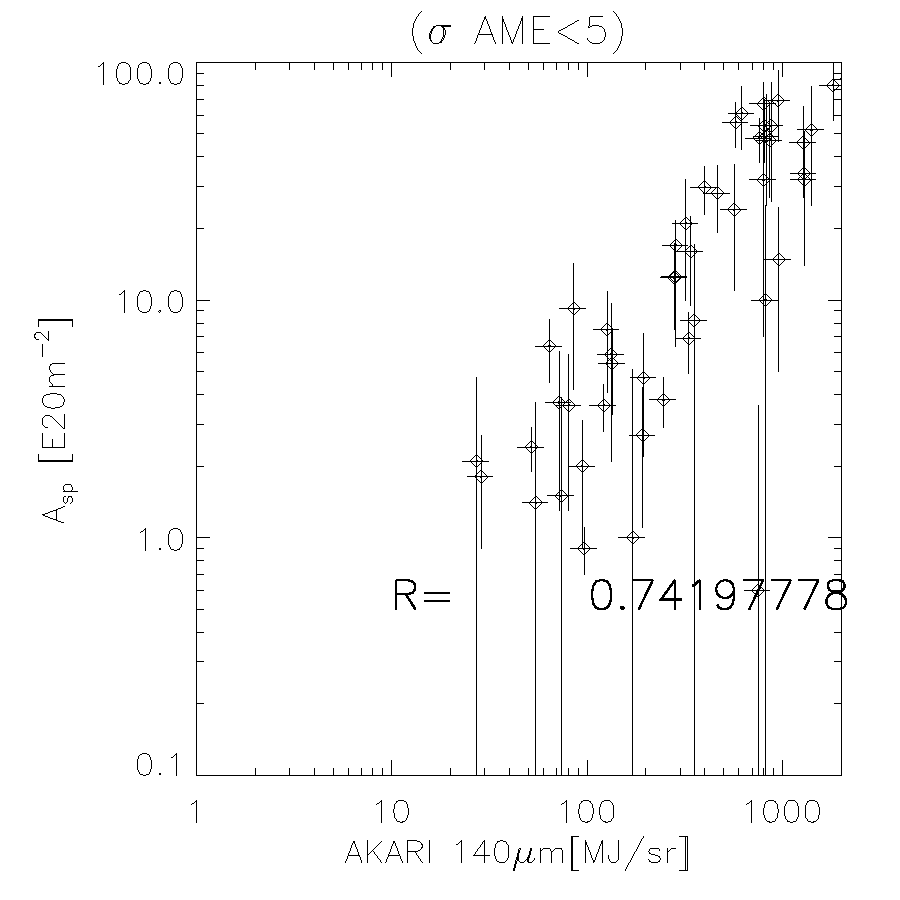
\includegraphics[width=50mm]{IRIntMWAmp/akari140_Asp_nosp.pdf}
  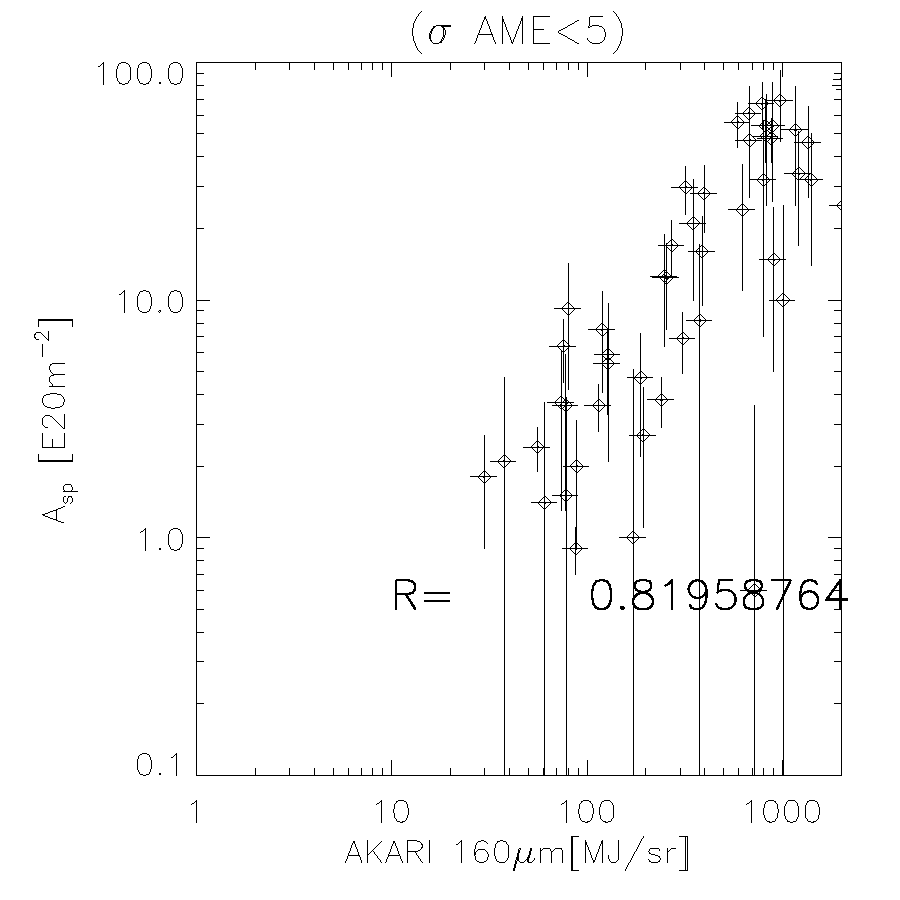
\includegraphics[width=50mm]{IRIntMWAmp/akari160_Asp_nosp.pdf}
  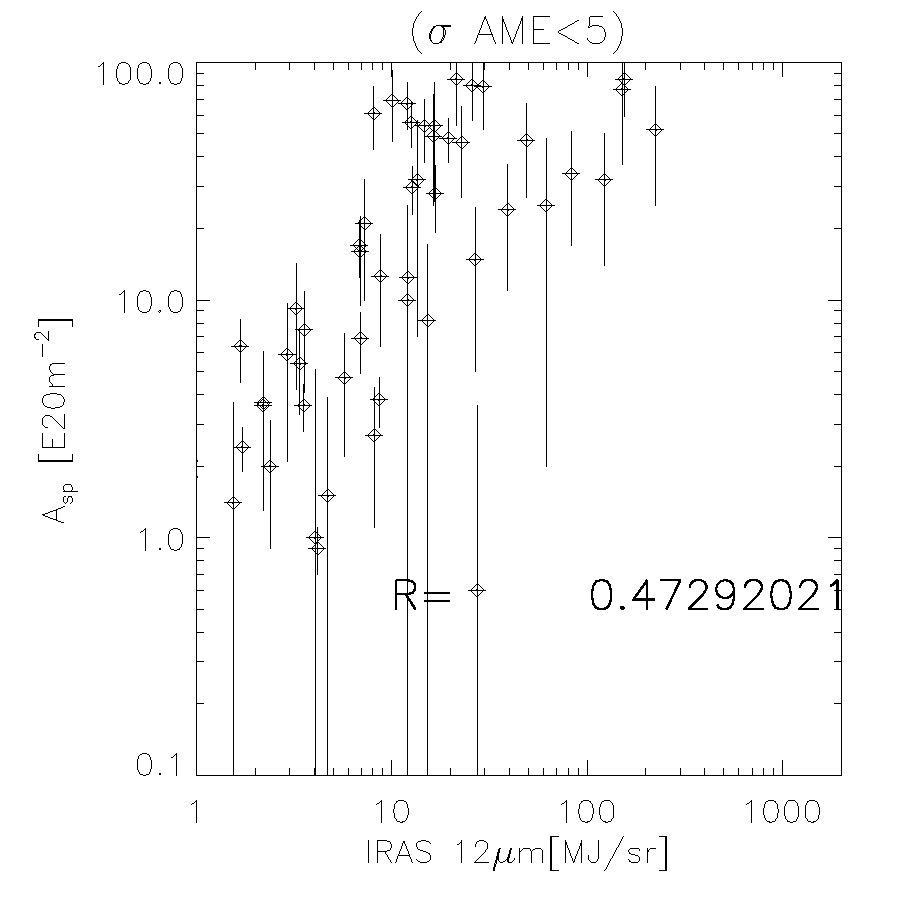
\includegraphics[width=50mm]{IRIntMWAmp/iras12_Asp_nosp.pdf}
  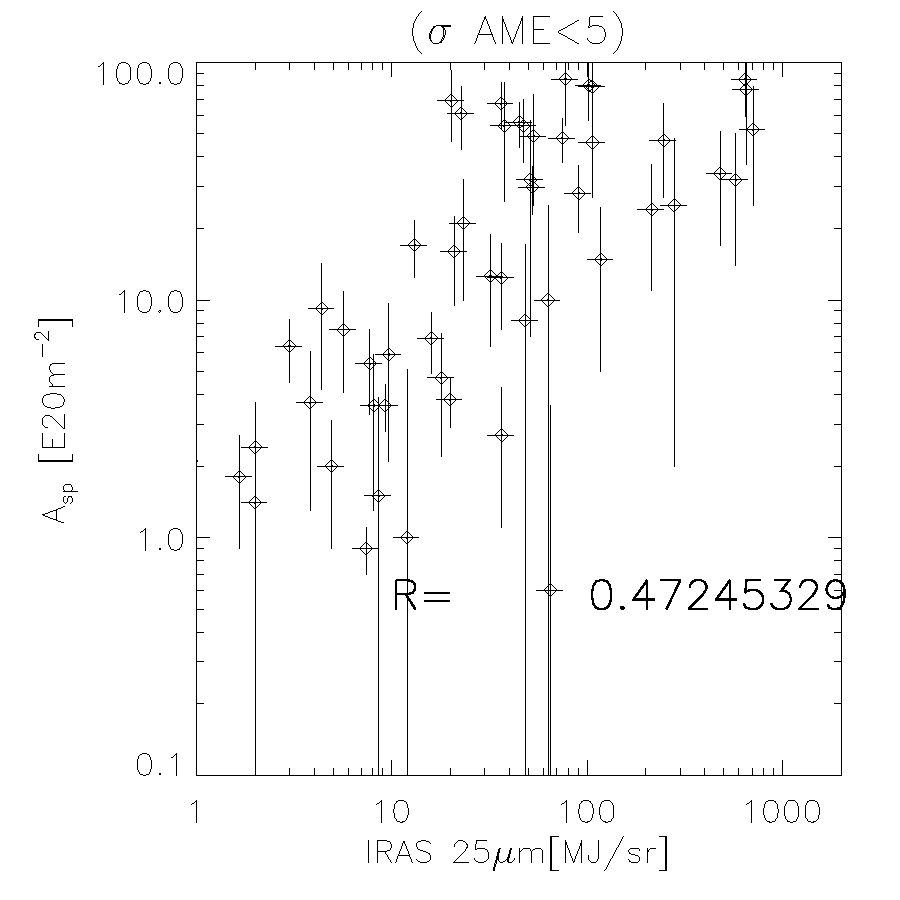
\includegraphics[width=50mm]{IRIntMWAmp/iras25_Asp_nosp.pdf}
  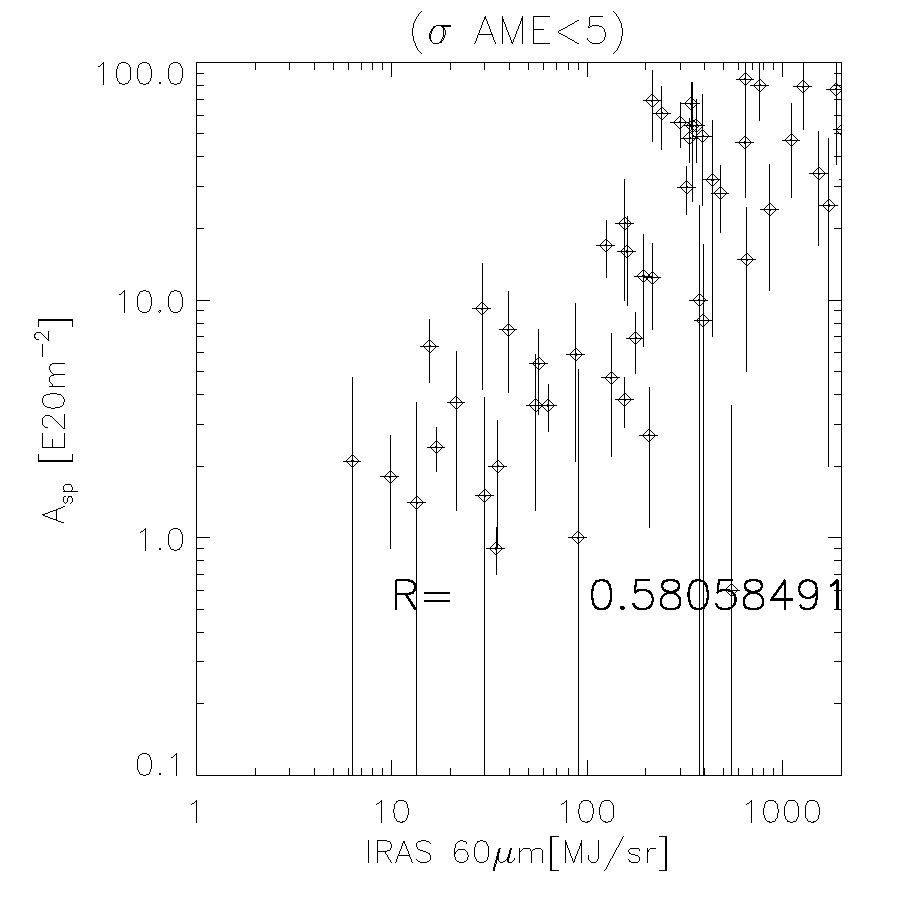
\includegraphics[width=50mm]{IRIntMWAmp/iras60_Asp_nosp.pdf}
  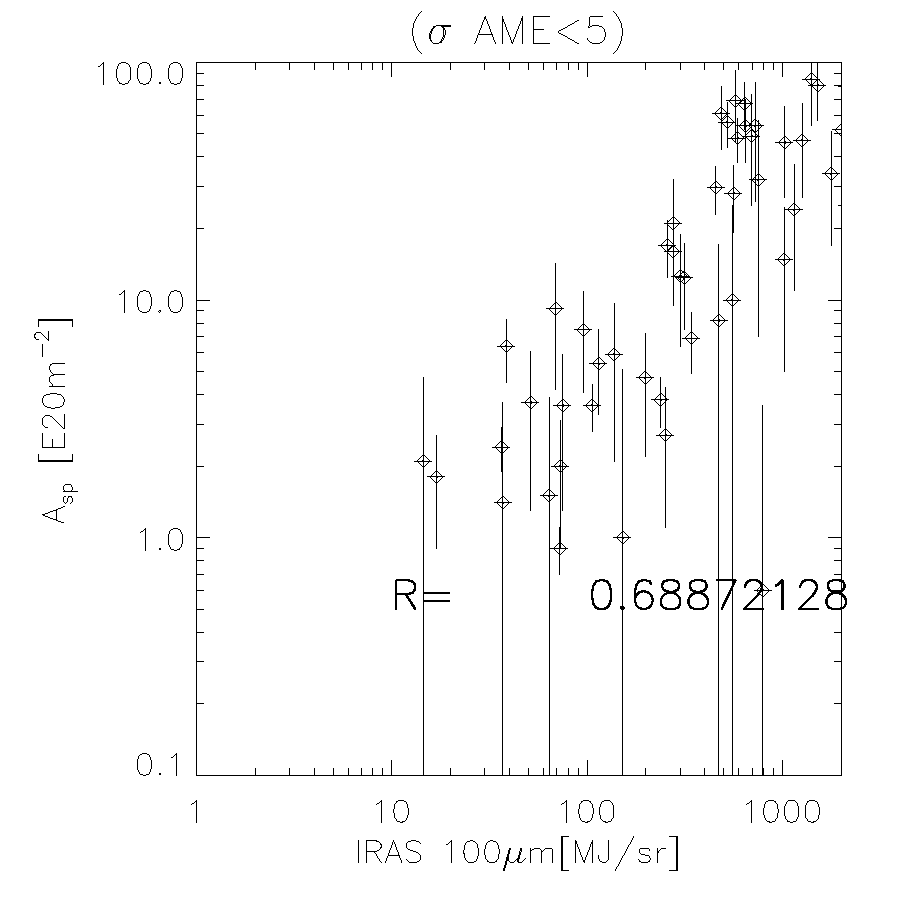
\includegraphics[width=50mm]{IRIntMWAmp/iras100_Asp_nosp.pdf}
  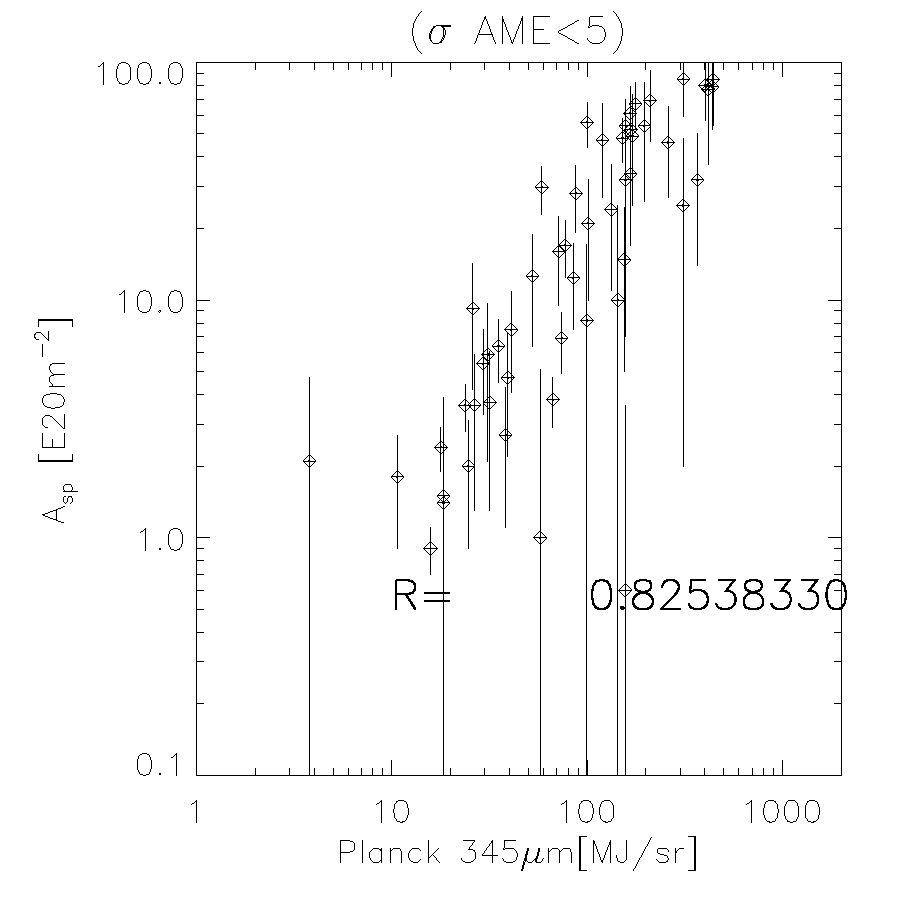
\includegraphics[width=50mm]{IRIntMWAmp/planck857_Asp_nosp.pdf}
  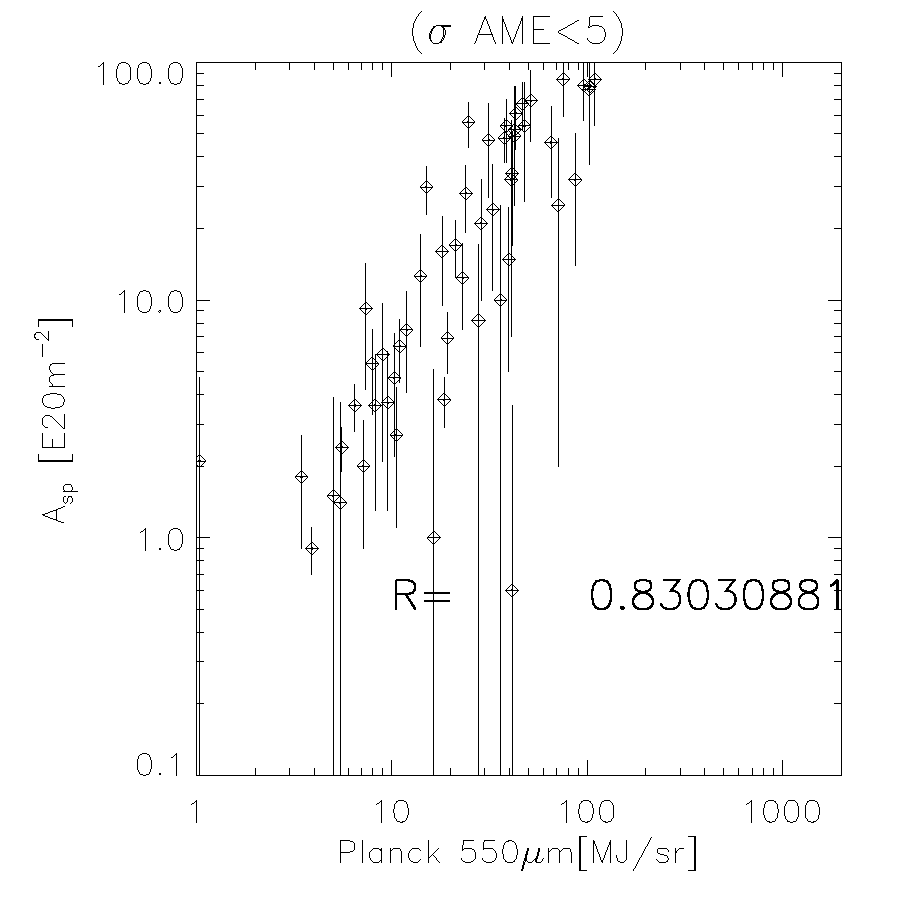
\includegraphics[width=50mm]{IRIntMWAmp/planck545_Asp_nosp.pdf}
\caption{These plots show the $I({\lambda})$ vs, $A_{sp}$ when only the non-significant AME regions are considered ($\sigma AME < 5$). 
}
\label{fig:IRIntMWAmpnosp}
\end{figure}

\subsection{Average Infrared Intensity $I({\lambda})$ Scaled by $G0$ vs. AME Amplitude $A_{sp}$}
     Following the analysis of previous studies, we plotted these regions again though with the intensities scaled by the $G0$ value of each region. $G0$ is the ISRF of a region relative to that of the solar neighborhood, and is determined from the modified blackbody fitting described in Chapter 2. 
\begin{figure}[!htb]
\centering
 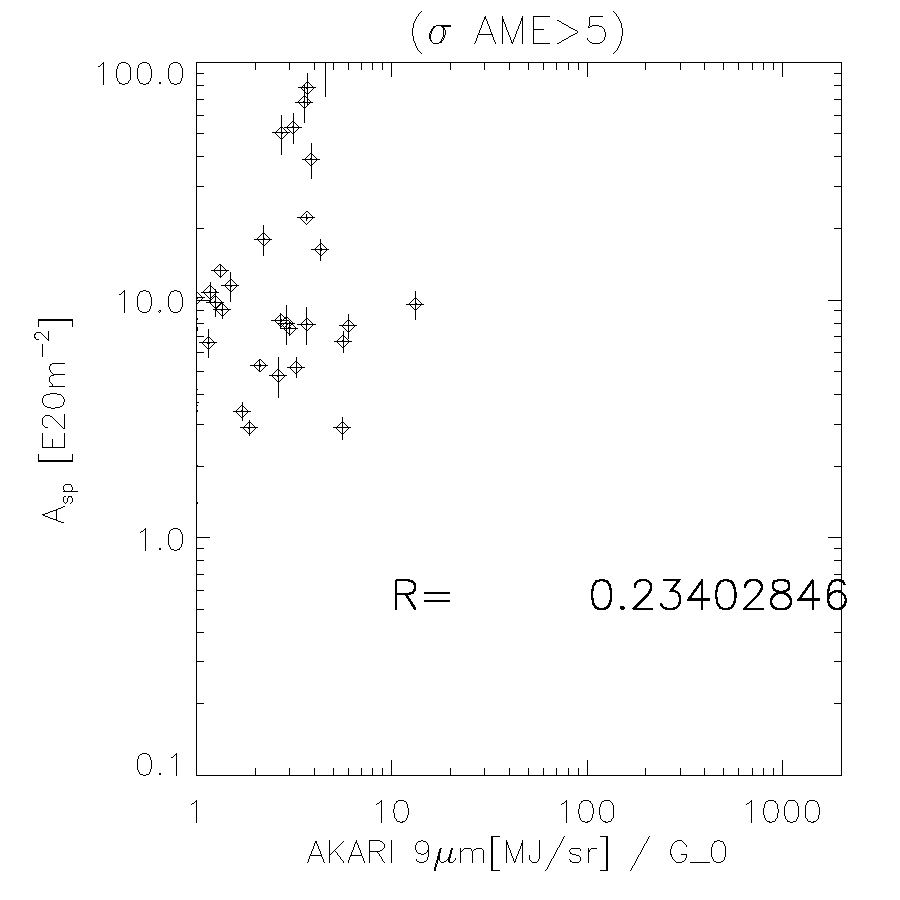
\includegraphics[width=50mm]{IRIntG0MWAmp/akari9G0_Asp_sp.pdf}
  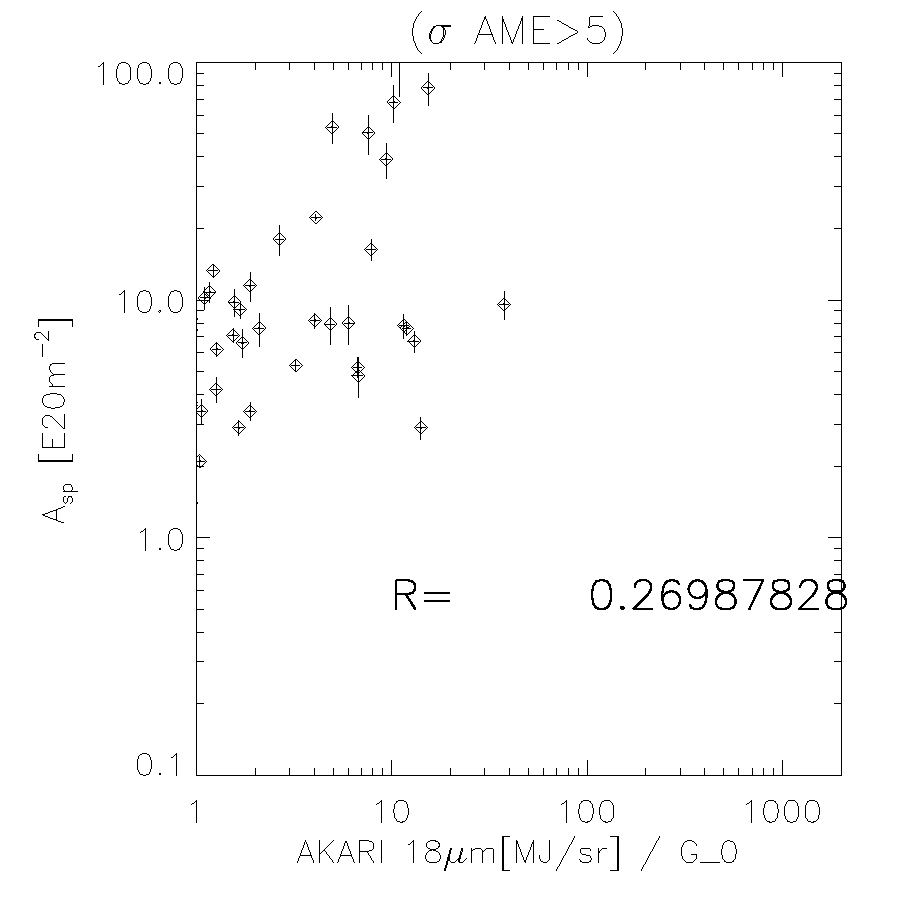
\includegraphics[width=50mm]{IRIntG0MWAmp/akari18G0_Asp_sp.pdf}
  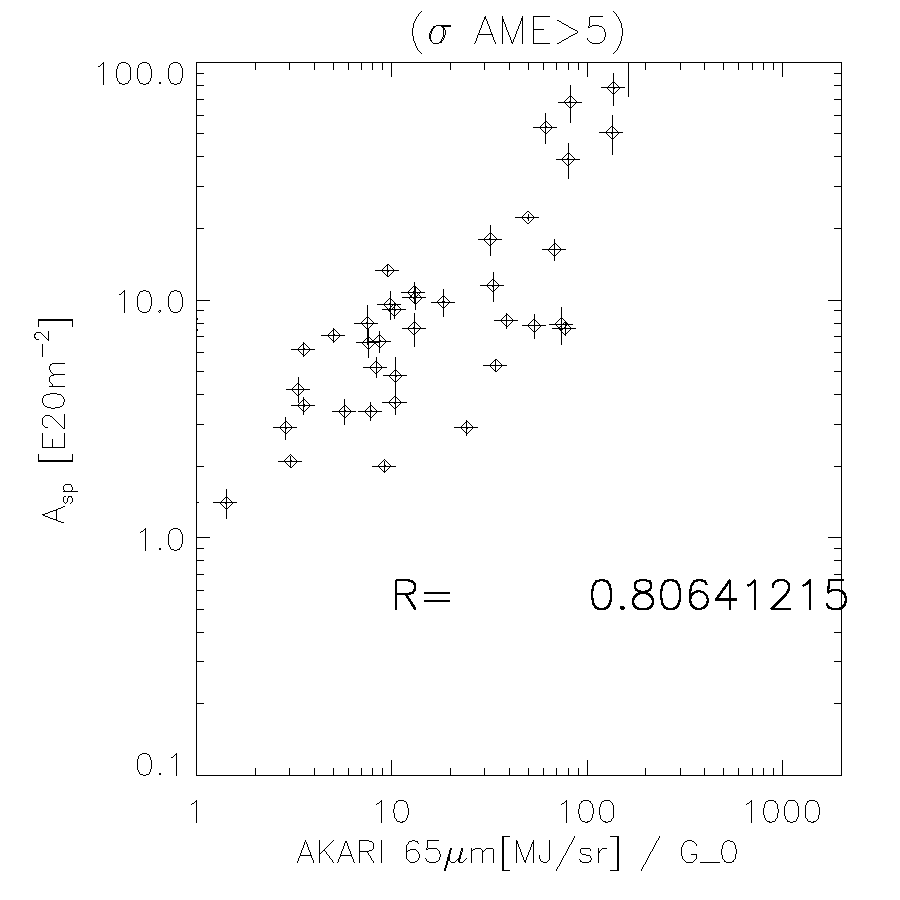
\includegraphics[width=50mm]{IRIntG0MWAmp/akari65G0_Asp_sp.pdf}
  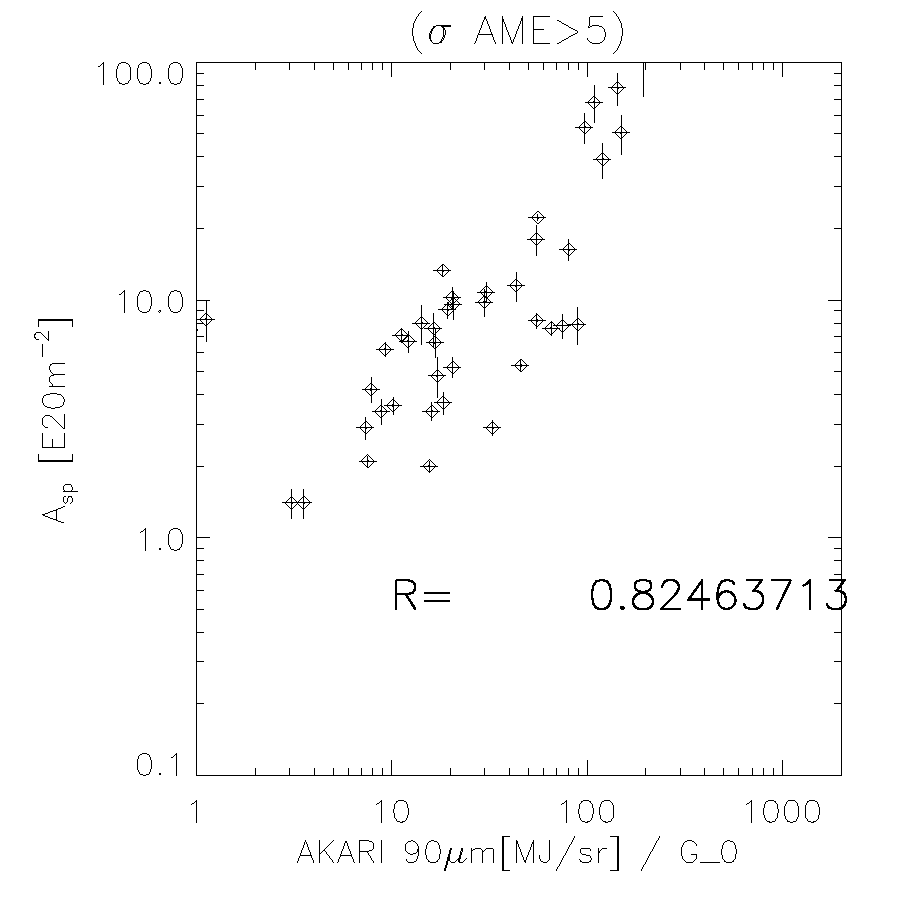
\includegraphics[width=50mm]{IRIntG0MWAmp/akari90G0_Asp_sp.pdf}
  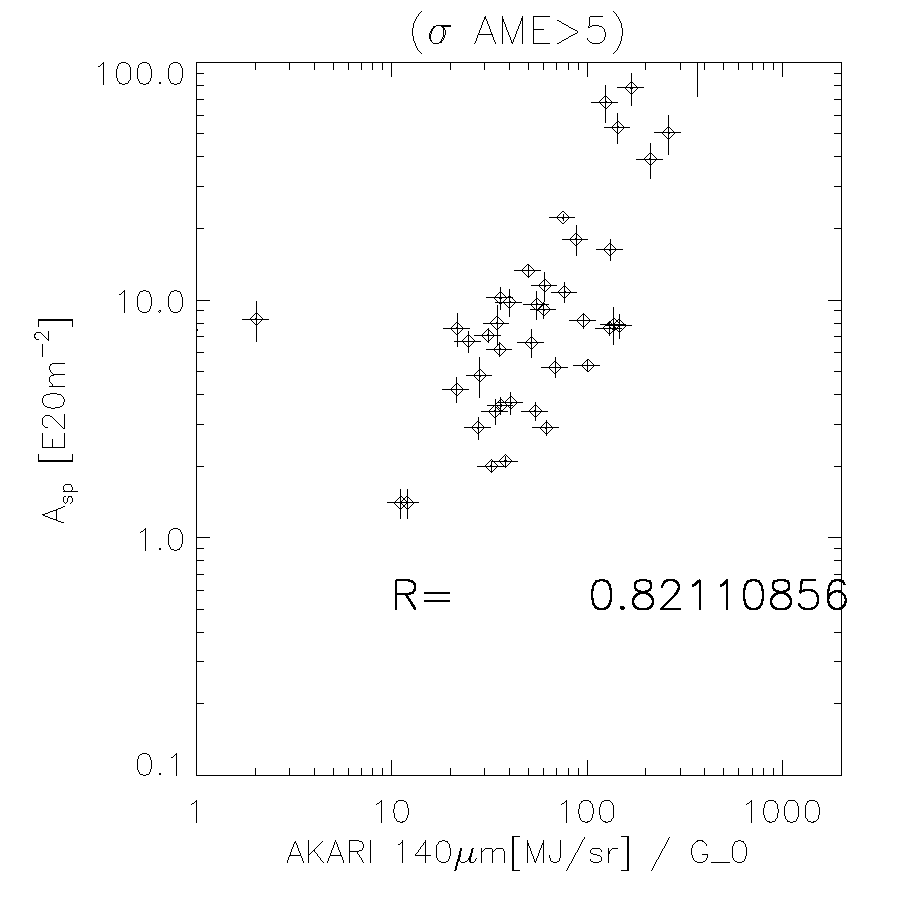
\includegraphics[width=50mm]{IRIntG0MWAmp/akari140G0_Asp_sp.pdf}
  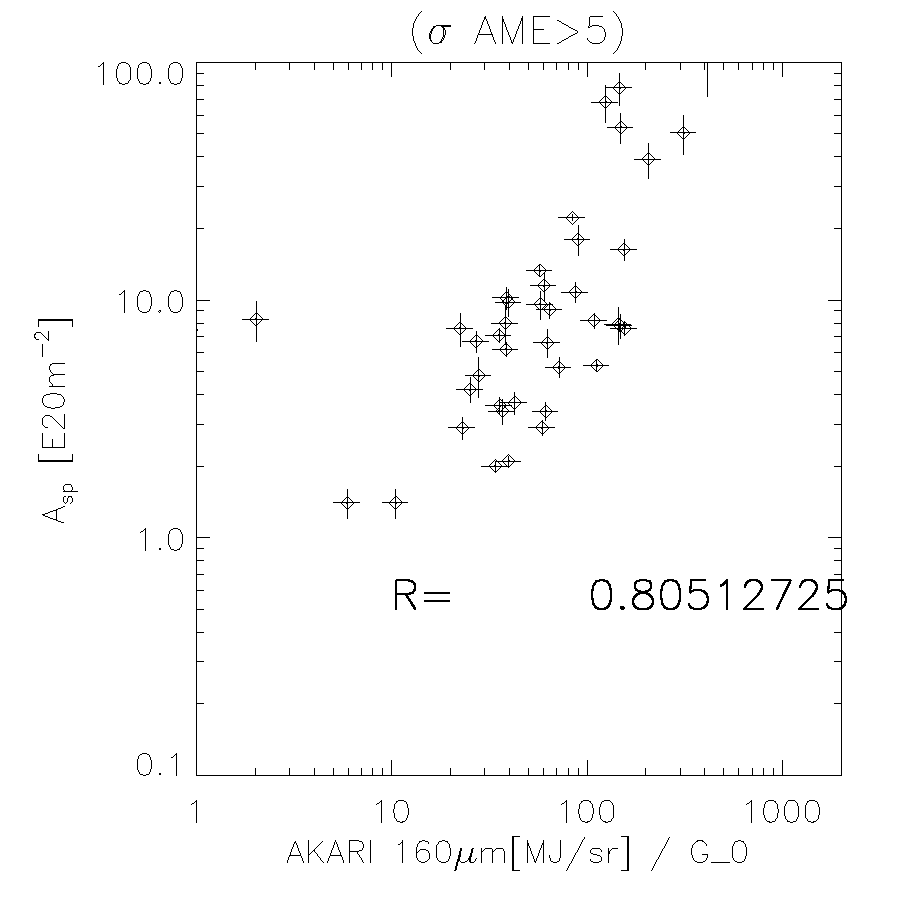
\includegraphics[width=50mm]{IRIntG0MWAmp/akari160G0_Asp_sp.pdf}
  \includegraphics[width=50mm]{IRIntG0MWAmp/iras12G0_Asp_sp.pdf}
  \includegraphics[width=50mm]{IRIntG0MWAmp/iras25G0_Asp_sp.pdf}
  \includegraphics[width=50mm]{IRIntG0MWAmp/iras60G0_Asp_sp.pdf}
  \includegraphics[width=50mm]{IRIntG0MWAmp/iras100G0_Asp_sp.pdf}
  \includegraphics[width=50mm]{IRIntG0MWAmp/planck857G0_Asp_sp.pdf}
  \includegraphics[width=50mm]{IRIntG0MWAmp/planck545G0_Asp_sp.pdf}
\caption{In these figures, the band-by-band correlation test of $I({\lambda})$ vs. $A_{sp}$ is repeated, dividing $I({\lambda})$ by $G0$. Only significant AME regions are considered here ($\sigma AME < 5$). This case shows the weakest correlation of AKARI 9~$\mu$m with $A_{sp}$.
}
\label{fig:IRIntG0MWAmpsp}
\end{figure}
\begin{figure}[!htb]
\centering
 \includegraphics[width=50mm]{IRIntG0MWAmp/akari9G0_Asp_nosp.pdf}
  \includegraphics[width=50mm]{IRIntG0MWAmp/akari18G0_Asp_nosp.pdf}
  \includegraphics[width=50mm]{IRIntG0MWAmp/akari65G0_Asp_nosp.pdf}
  \includegraphics[width=50mm]{IRIntG0MWAmp/akari90G0_Asp_nosp.pdf}
  \includegraphics[width=50mm]{IRIntG0MWAmp/akari140G0_Asp_nosp.pdf}
  \includegraphics[width=50mm]{IRIntG0MWAmp/akari160G0_Asp_nosp.pdf}
  \includegraphics[width=50mm]{IRIntG0MWAmp/iras12G0_Asp_nosp.pdf}
  \includegraphics[width=50mm]{IRIntG0MWAmp/iras25G0_Asp_nosp.pdf}
  \includegraphics[width=50mm]{IRIntG0MWAmp/iras60G0_Asp_nosp.pdf}
  \includegraphics[width=50mm]{IRIntG0MWAmp/iras100G0_Asp_nosp.pdf}
  \includegraphics[width=50mm]{IRIntG0MWAmp/planck857G0_Asp_nosp.pdf}
  \includegraphics[width=50mm]{IRIntG0MWAmp/planck545G0_Asp_nosp.pdf}
\caption{In these figures, the band-by-band correlation test of $I({\lambda})$ vs. $A_{sp}$ is repeated, dividing $I({\lambda})$ by $G0$. Only non-significant AME regions are plotted here. This case shows a similar correlation factor across all of the bands. Interestingly,  the AKARI 9~$\mu$m with $A_{sp}$ correlation is stronger here than for the $\sigma AME > 5$ case.
}
\label{fig:IRIntG0MWAmpnosp}
\end{figure}
     As noted in Chapter 1, previous studies found that the AME generally correlates at dust-related IR wavelengths. We see the same overall pattern in the present study. However, contrary to previous works, we find that the correlation is not improved at the small-grain-related MIR wavelengths.
     Both PCXV and \cite{ysard10b} found that the correlations improved after dividing the IR photometric data by $G0$. We have repeated that calculation here using the average $G0$ of ROI, obtained from our a modified blackbody fitting results (with $\beta$ = 2). We find generally that all of the correlations with $A_{sp}$ weaken after dividing by $G0$. 
     In order to get a finer understanding of the IR/$G0$ vs. $A_{sp}$ variations, we again followed in the method of PCXV by separately plotting regions which are well-fitted by a spinning dust model ($\sigma AME>5$) vs. regions not well fitted by a spinning dust model ($\sigma AME<5$). The results are tabulated below.
\begin{table}[!htb]
\caption{Correlation Coefficients ($R$) of $I({\lambda})$ vs. $A_{sp}$ for 98 AME Regions} \label{IRvsAspTab}
\centering
\begin{tabular}{lrrrr}
\toprule
Wavelength ($\mu$m)	&$A_{sp}$ vs. $I({\lambda})$)	&$A_{sp}$ vs. $I({\lambda})$	&$A_{sp}$ vs. $I({\lambda}$/$G0$)	&$A_{sp}$ vs. $I({\lambda})$/$G0$ \\ 
    &$\sigma AME>5$  &$\sigma AME<5$ &$\sigma AME>5$  &$\sigma AME<5$      \\
\midrule
9	&0.703	&0.568	&0.234	&0.562 \\
12	&0.735	&0.473	&0.270	&0.601 \\
18	&0.649	&0.457	&0.589	&0.558 \\
25	&0.659	&0.472	&0.662	&0.616 \\
60	&0.761	&0.580	&0.797	&0.641 \\
65	&0.811	&0.635	&0.806	&0.701 \\
90	&0.851	&0.729	&0.824	&0.728 \\
100	&0.871	&0.689	&0.812	&0.658 \\
140	&0.944	&0.742	&0.821	&0.649 \\
160	&0.965	&0.820	&0.805	&0.630 \\
345	&0.944	&0.825	&0.441	&0.597 \\
550	&0.920	&0.830	&0.290	&0.571 \\
\bottomrule
\end{tabular}
\end{table}

\subsection{AKARI 9:18~$\mu$m Ratio vs. AME$\sigma$}
     We described a preliminary result in proceedings at the 2014 \textit{Universe in the Light of AKARI} conference at Oxford, regarding the AKARI/IRC 9 to 18~$\mu$m band ratio, R(9,18), for 10 PCXV AME regions (Table 3.2), Figure 3.7) (Bell et al., in prep). Regions of higher AME significance tended to have a R(9,18) value above unity. This relationship was revisited in the current study, for all 98 PCXV AME regions, and the updated result is shown in Figure 3.8. The previous result does not hold-up to the full sample, as we cannot find a clear trend between R(9,18) and AME significance.
\begin{table}[!htb]
\label{tab:R918a}
\caption{IRC average intensities and 9 to 18~$\mu$m band ratios of AME candidate regions}
\centering
\begin{tabular}{lrrrr}
\toprule
Target           & AME$\sigma$       & R(9,18)          &  9~$\mu$m MJysr$^{-1}$        & 18~$\mu$m MJysr$^{-1}$ \\
\midrule
G353.05+16.09   & 29.8	     & 1.37   &  0.134       & 0.098 \\
G160.26-18.62	 & 17.4	     & 1.27   &  0.0186      & 0.0147 \\
G004.24+18.09   & 15.6      & 1.10   &  0.00254     & 0.0023 \\
G107.20+05.20	 & 9.9       & 1.88   &  0.0955      & 0.0507 \\
G173.63+02.80	 & 5.6       & 1.04   &  0.0244      & 0.0235 \\
G305.27+00.15	 & 6.3       & 0.47   &  0.276       & 0.583 \\ 
G209.01-19.38 & 1.9       & 0.57   &  0.0373      & 0.065 \\
G123.13-06.28 & 1.8       & 0.09   &  0.00753     & 0.0828 \\
G040.52+02.53 & 0.2       & 1.43   &  0.0596      & 0.0418 \\
G289.80-01.15 & 0         & 0.73   &  0.0887      & 0.121 \\
\bottomrule
\end{tabular}
\end{table}
\begin{figure}[!htb]
\label{fig:R918PlotA}
\centering
\includegraphics[angle=0,width=100mm]{EPS/bell_fig1.pdf}
\caption{The AKARI/IRC 9 to 18~$\mu$m intensity ratios for several AME regions (see Table 3.2) against each region's AME$\sigma$ value, taken from Planck Collaboration XV.}
\end{figure}
\begin{figure}[!htb]
\label{fig:R918PlotB}
\centering
\includegraphics[angle=0,width=100mm]{EPS/IRCratio_vs_AMEsigma_betafix.pdf}
\caption{The AKARI/IRC 9 to 18~$\mu$m intensity ratios for all 98 AME regions from PCXV against each region's $\sigma$AME value. The determination of the average R(9,18) value is slightly different from our previous analysis. In the present study we take an average of the non-background pixels. The data used to determine R(9,18) is the same as described in Section 2.4. In the previous calculation using only 10 AME regions, (Figure 3.6), we used circular aperture photometry on the un-smoothed IRC data. }
\end{figure}

\chapter{Discussion}
  \label{chap:Discussion}
  \section{A Correlation is not Enough}
     As noted by Jones at al. (2013) at the \textit{Life Cycle of Cosmic Dust} conference in Taipei, material in the galaxy tends to correlate with other material in the galaxy. In other words, the greatest challenge of this type of study is not in finding a correlation between PAHs or any other dust component and  AME, indeed such a correlation is expected and easy to find. The challenge is in finding second-order variations that relate to the AME and spinning dust. For example, even if we had a truly perfect survey of pure PAH emission in the galaxy, finding that it correlates with AME would not be particularly useful. We expect that dense regions of the ISM will contain all major components of dust / gas in some proportions. There may be regions where PAHs, for example, are perhaps being destroyed due to environmental conditions, but in general the major components of dust and gas will trace one another. 
     What we need to find, in order to make any clear conclusion, is how the different components vary with respect to one another. This challenge has certainly presented itself in this thesis project. While the notion of a possible PAH-AME connection was motivating, it is not so easy to establish. There are a few fundamental questions involved:
  
  1.) What influences the UIR/PAH bands? Do ``pure" PAHs exist in significant abundances? 
  
     A mixture of PAHs and other PAH-class aromatic molecules could mean a wide mixture of AME carriers, perhaps being rotationally excited to different extents under different conditions. This could mean that even if the PAH band carriers are also the carriers of the AME, a clear correlation with the AME may remain elusive. 
  
  2.) Are the UIR / PAH band carriers also the carriers of the AME? Are they the only carriers?

    Even if the AME is spinning dust, there is the possibility that the PAH band carriers are not the AME carriers. If they are, they may not be the only carriers. For example, other very small grains not strongly covered by a PAH dominated survey like AKARI/IRC 9~$\mu$m could be contributing spinning dust emission.
  
  3.) What is the major contributor to the AME observed in these regions?
  
  Even if we are able to understand completely the nature of the PAH bands emission, it may still be the case that we do not fully understand the mechanisms which can produce AME. For example, the magnetic dust contribution is still uncertain. Free-free emission is also sometimes difficult to quantify. For the diffuse sky, it has been shown that there is not a clearly explained model that can explain the AME \citep{hfi14viii}.
  
  4.) What are the environmental factors that influence AME?
  
     We must remember that simply the presence of possible carriers of AME may not influence the observed AME. Whether spinning dust or magnetic dust, if environmental conditions like ISRF, column density, or metallicity are more important for producing an environment that promotes AME, then it is not sufficient only to identify the carriers. In this way too, me may not see any especially strong relationship among even a PAH-survey. 
     With these questions in mind, we have performed an examination of the data across an expansive wavelength range. The maps and instruments involved are very advanced and in some cases quite specialized in their objective, like the PAH band tracing AKARI/IRC 9~$\mu$m survey \citep{irc07,ishihara10}, or the peak thermal emission tracing FIS surveys \citep{doi12}, or the Planck/HFI data tracing primarily cold dust. We discuss the results of this comparison below. This is the first time AKARI, IRAS, and HFI data have been combined for AME studies.
  
  \section{$A_{sp}$ vs. $\tau_{250}$}
     The moderate trend found in Chapter 3 between $\tau_{250}$ and $A_{sp}$ suggests a dust-AME relationship (R = 0.87) for AME regions. This result is as expected, assuming that AME arises from dust. As was described by \cite{draine98a} via Equation \ref{eq:Pspin} that more spinning grains would directly relate to a higher amplitude of spinning dust emission. Our result follows the result of both PCXV and \cite{ysard10a}. We find that the result is similar non-AME regions (R=0.77), in agreement with PCXV.
     In the case of non-AME regions,  we must use some caution. The authors of PCXV emphasize that $A_{sp}$ is only valid as a measure of column density of spinning dust if their model is correct for a given ROI. If the regions from which $A_{sp}$ is determined do not have an SED that agrees with the spinning dust model, the correlation test result has less meaning. In such a case, $A_{sp}$ is more likely to trace free-free emission or thermal dust emission which was not completely removed from the microwave data (``residual residual" emission). However, even in this case we would expect that $A_{sp}$ should increase with $\tau_{250}$. We note that the correlation of $\tau_{250}$ with $A_{sp}$ is stronger for significant AME regions. However, this may not be a significant difference as the error bars of $A_{sp}$ for non-AME regions are larger by definition. Moreover, the sample size of non-AME regions is larger than the sample size of AME regions. 
     Perhaps a re-determination of $A_{sp}$ and $\sigma$AME for each ROI, with adjustments made to the spinning dust model on a region-by-region basis, could more powerfully test for a $\tau_{250}$ vs. AME relationship. Another option is to repeat the study with full-SED modelling. As of the time of this writing, template dust models for the model used by \cite{galliano11} should soon be available. We hope to include a full-SED modelling based on these templates, as well as modelling based on the DustEM code by \cite{dustem11}. In this way we can obtain the relative abundances of each of the major dust components (aromatics, carbonaceous grains, silicate grains) simultaneously. This would offer a more powerful comparison of dust properties vs. the AME. 

\section{Comparison of AME with IRC Data}
     The full dust SED modelling seems to be even more necessary, given the result of the MIR vs. $A_{sp}$ plots. A spinning dust model suggests that the correlations should become clearer after dividing $I_{MIR}(\lambda)$ by $G0$. This is because the spinning dust intensity is not expected to depend on $G0$. Also, dividing $I_{MIR}(\lambda)$ by $G0$ should more closely trace the abundance of PAHs and VSGs. Thus the trend should be more clear. However we find that the correlation between MIR and $A_sp$ becomes much worse after scaling by $G0$. This suggests perhaps that the spinning PAH hypothesis is not correct, or at least that the role of $G0$ in producing spinning dust may be more important than initially thought.
     \cite{tibbs12b} find that the AME in the HII region RCW175 does not show a correlation between AME and small dust emission. PCXV find that RCW175 does not have a high AME significance in the Planck data, thus we cannot compare these results to \cite{tibbs12b} directly. However we have shown that the general trend for the 98 ROIs is that a weaker correlation is seen with the short-wavelength bands (both the 9~$\mu$m survey which traces PAHs heavily and those which trace primarily other VSG emission, like IRAS 12~$\mu$m and AKARI 18~$\mu$m vs. bands dominated by emission from the FIR modified blackbody. 
 
\subsection{$\tau_{250}$ vs. $A_{sp}$ Compared to AKARI 9~$\mu$m vs. AME}
     The lack of a clear PAH-band vs. $A_{sp}$ trend is especially interesting. This could indicate that non-PAH small grains are more dominant in carrying the AME, or that the simple averaged 9~$\mu$m intensity is not sufficient to access a relation with AME. A possible systematic explanation for the weaker correlation in the IRC data is the lack of a sophisticated zody-subtraction. Background subtraction was completed for the IRC data using a robust-mean subtraction (see Chapter \ref{chap:Data}). The zody model is still being perfected by Ishihara et al. (in prep.). Some of the calibration parameters of the IRC maps are also being redetermined. In any case we will re-run the analysis when the final IRC all-sky maps are released.     
 %     PCXV carried out their IR analysis IRAS bands only. Our result for the IRAS bands is similar to theirs. Variations may be due to the $G0$ and $A_{sp}$ values having been determined at much larger angular resolutions, with all of their data being smoothed to 1$\degree$.
  
\subsection{Magnetic dust emission: A remaining question}
     The magnetic dipole emission interpretation for AME cannot be ruled out, based on our analysis. Magnetic dust may be a substitute explanation for the AME, or possibly an overlapping explanation. Magnetic dipole emission from dust does not require PAHs. If the AME is connected more to $\tau_{250}$ than to $\tau_{MIR}$, that temperature fluctuations of magnetic grains is an interpretation that mus be explored further. We cannot offer a strong conclusion about magnetic dust here, but we leave it as an open question for future research.

\chapter{Summary
  \label{chap:Summary}}
     This thesis has presented one of the earliest efforts to conduct a multi-wavelength investigation using all 7 AKARI all-sky surveys along with IRAS and Planck data. The wavelength range spans 9~$\mu$m to 545~$\mu$m. The purpose was to gather information from all major dust components, from aromatic organic molecules (Section \ref{PAHhypothesis}) to larger carbonaceous and silicate grains. Chapter \ref{chap:Introduction} gives a general overview of the ISM and interstellar dust, and the basic physics of the AME and galactic foreground.
     A total of 98 regions from PCXV were examined for the first time at AKARI wavelengths. Most importantly, the AKARI/IRC 9~$\mu$m all-sky data was inspected. This survey contains one of the most complete data-sets for looking at the PAH/UIR bands over a very large spatial range. The PAH band photometry was considered critical because one of the primary suspects for an AME carrier is the PAH family of molecules (Section \ref{spinningdust}).
     Chapter \ref{chap:Data} reviews the data sources used for this study. The extraction of sources and their processing are also described, including the PSF smoothing, pixel regridding, SED extraction, modified blackbody fitting, and color-correction. A major component of the data processing is the smoothing of the data to the largest PSF, Planck/HFI 545~GHz at 4.7$'$. A major limitation of the processing is that the finer resolution of AKARI/IRC and FIS is not able to be utilized due to the PSF smoothing. We can take advantage only of the overall spatial coverage, and additional sampling positions along the dust SED in the MIR and FIR (especially in the PAH domain, and around the peak of the thermal emission curve). 
%A case study of one region, $\rho$~Ophiuchi is presented to demonstrate the resolving capability of AKARI (and its uniqueness as an all-sky data set at such fine resolution).
     Chapter 3 presents several attempts to illuminate possible patterns between the IR photometry and the AME/spinning dust parameters derived by PCXV which examined lower-frequency data not used in this thesis, i.e. Planck/LFI \citep{lfi14ii}. The methodology for deriving estimates of dust properties from the SEDs is presented, such as the optical depth at 250~$\mu$m (Equation 3.1.1). Plots of each photometric band's average intensity against the AME amplitude derived by PCXV are presented. The same plots, though with the IR intensities divided by the ISRF scaling factor $G0$ are also included.
     In Chapter \ref{chap:Discussion}, a lack of support for a spinning dust model in the current analysis is described. Ways in which the data might allow for a magnetic dust contribution is described, as well as a possibility that the results are due to varying methods between the current analysis and that of preceding works, PCXV and \cite{ysard10a}. The contradicting results of this study and the same analysis performed by the previous works' authors is of the most importance. Prior to this analysis it was generally accepted that shorter wavelength data correlates more tightly with AME than longer wavelength dust SED data. We do not find the same pattern, especially in the case of the AKARI/IRC 9~$\mu$m. We also fail to find that the correlations become stronger after scaling by $G0$.
     In the same way, the plots which show FIR-emitting dust optical depth $\tau_{250}$ vs. the AME indicate a general trend between dust column density and AME amplitude. A slightly stronger trend is seen with the significant AME regions than with non-significant AME regions. This result agrees with that of previous works. The implications were discussed, as well as the disagreement with the IRC data. The question of contribution of magnetic dipole emission from dust to the AME cannot be answered here, but we do argue that it is necessary to fully explore the magnetic dust hypothesis.

%%% appendix %%%
\appendix
\chapter*{Appendix A:
Modified Blackbody Fitting Images}
\addcontentsline{toc}{chapter}{Appendix A}
This appendix presents the complete set of the modified blackbody fitting results. In Appendix A, the fitted-parameter images of each region are presented. The far left panel shows the optical depth at 250~$\mu$m, $\tau_{250}$. center-left is the fitted temperature, $T$, center-right is the ISRF strength in terms of $G0$, and the far-right panel shows the reduced $\chi^2$ result of each pixel. Masked pixels are black. Each region's coordinates are given in the upper-left corner of each set of panels. Appendix B shows the averaged result of the modified blackbody fitting of each of these regions, in terms of an SED plot.

\begin{figure}[!htb]
\centering
\includegraphics[trim=0 2mm 0 0, clip, width=190mm]{appA/appA_96.pdf}
\includegraphics[trim=0 2mm 0 0, clip, width=190mm]{appA/appA_97.pdf}
\end{figure}

\begin{figure}
\centering
\includegraphics[trim=0 2mm 0 0, clip, width=190mm]{appA/appA_0.pdf}
\includegraphics[trim=0 2mm 0 0, clip, width=190mm]{appA/appA_1.pdf}
\includegraphics[trim=0 2mm 0 0, clip, width=190mm]{appA/appA_2.pdf}
\includegraphics[trim=0 2mm 0 0, clip, width=190mm]{appA/appA_3.pdf}
\includegraphics[trim=0 2mm 0 0, clip, width=190mm]{appA/appA_4.pdf}
\includegraphics[trim=0 2mm 0 0, clip, width=190mm]{appA/appA_5.pdf}

  \end{figure}
  
  \begin{figure}
\centering
\includegraphics[trim=0 2mm 0 0, clip, width=190mm]{appA/appA_6.pdf}  
\includegraphics[trim=0 2mm 0 0, clip, width=190mm]{appA/appA_7.pdf}
\includegraphics[trim=0 2mm 0 0, clip, width=190mm]{appA/appA_8.pdf}
\includegraphics[trim=0 2mm 0 0, clip, width=190mm]{appA/appA_9.pdf}
\includegraphics[trim=0 2mm 0 0, clip, width=190mm]{appA/appA_10.pdf}
\includegraphics[trim=0 2mm 0 0, clip, width=190mm]{appA/appA_11.pdf}
  \end{figure}
  
  \begin{figure}
\centering
\includegraphics[trim=0 2mm 0 0, clip, width=190mm]{appA/appA_12.pdf}
\includegraphics[trim=0 2mm 0 0, clip, width=190mm]{appA/appA_13.pdf}
\includegraphics[trim=0 2mm 0 0, clip, width=190mm]{appA/appA_14.pdf}
\includegraphics[trim=0 2mm 0 0, clip, width=190mm]{appA/appA_15.pdf}
\includegraphics[trim=0 2mm 0 0, clip, width=190mm]{appA/appA_16.pdf}
\includegraphics[trim=0 2mm 0 0, clip, width=190mm]{appA/appA_17.pdf}
  \end{figure}
  
  \begin{figure}
\centering
\includegraphics[trim=0 2mm 0 0, clip, width=190mm]{appA/appA_18.pdf}
\includegraphics[trim=0 2mm 0 0, clip, width=190mm]{appA/appA_19.pdf}
\includegraphics[trim=0 2mm 0 0, clip, width=190mm]{appA/appA_20.pdf}
\includegraphics[trim=0 2mm 0 0, clip, width=190mm]{appA/appA_21.pdf}
\includegraphics[trim=0 2mm 0 0, clip, width=190mm]{appA/appA_22.pdf}
\includegraphics[trim=0 2mm 0 0, clip, width=190mm]{appA/appA_23.pdf}
  \end{figure}
  
  \begin{figure}
\centering
\includegraphics[trim=0 2mm 0 0, clip, width=190mm]{appA/appA_24.pdf}
\includegraphics[trim=0 2mm 0 0, clip, width=190mm]{appA/appA_25.pdf}
\includegraphics[trim=0 2mm 0 0, clip, width=190mm]{appA/appA_26.pdf}
\includegraphics[trim=0 2mm 0 0, clip, width=190mm]{appA/appA_27.pdf}
\includegraphics[trim=0 2mm 0 0, clip, width=190mm]{appA/appA_28.pdf}
\includegraphics[trim=0 2mm 0 0, clip, width=190mm]{appA/appA_29.pdf}
  \end{figure}
  
  \begin{figure}
\centering
\includegraphics[trim=0 2mm 0 0, clip, width=190mm]{appA/appA_30.pdf}
\includegraphics[trim=0 2mm 0 0, clip, width=190mm]{appA/appA_31.pdf}
\includegraphics[trim=0 2mm 0 0, clip, width=190mm]{appA/appA_32.pdf}
\includegraphics[trim=0 2mm 0 0, clip, width=190mm]{appA/appA_33.pdf}
\includegraphics[trim=0 2mm 0 0, clip, width=190mm]{appA/appA_34.pdf}
\includegraphics[trim=0 2mm 0 0, clip, width=190mm]{appA/appA_35.pdf}
  \end{figure}
  
  \begin{figure}
\centering
\includegraphics[trim=0 2mm 0 0, clip, width=190mm]{appA/appA_36.pdf}
\includegraphics[trim=0 2mm 0 0, clip, width=190mm]{appA/appA_37.pdf}
\includegraphics[trim=0 2mm 0 0, clip, width=190mm]{appA/appA_38.pdf}
\includegraphics[trim=0 2mm 0 0, clip, width=190mm]{appA/appA_39.pdf}
\includegraphics[trim=0 2mm 0 0, clip, width=190mm]{appA/appA_40.pdf}
\includegraphics[trim=0 2mm 0 0, clip, width=190mm]{appA/appA_41.pdf}
  \end{figure}
  
  \begin{figure}
\centering
\includegraphics[trim=0 2mm 0 0, clip, width=190mm]{appA/appA_42.pdf}
\includegraphics[trim=0 2mm 0 0, clip, width=190mm]{appA/appA_43.pdf}
\includegraphics[trim=0 2mm 0 0, clip, width=190mm]{appA/appA_44.pdf}
\includegraphics[trim=0 2mm 0 0, clip, width=190mm]{appA/appA_45.pdf}
\includegraphics[trim=0 2mm 0 0, clip, width=190mm]{appA/appA_46.pdf}
\includegraphics[trim=0 2mm 0 0, clip, width=190mm]{appA/appA_47.pdf}
  \end{figure}
  
  \begin{figure}
\centering
\includegraphics[trim=0 2mm 0 0, clip, width=190mm]{appA/appA_48.pdf}
\includegraphics[trim=0 2mm 0 0, clip, width=190mm]{appA/appA_49.pdf}
\includegraphics[trim=0 2mm 0 0, clip, width=190mm]{appA/appA_50.pdf}
\includegraphics[trim=0 2mm 0 0, clip, width=190mm]{appA/appA_51.pdf}
\includegraphics[trim=0 2mm 0 0, clip, width=190mm]{appA/appA_52.pdf}
\includegraphics[trim=0 2mm 0 0, clip, width=190mm]{appA/appA_53.pdf}
  \end{figure}
  
  \begin{figure}
\centering
\includegraphics[trim=0 2mm 0 0, clip, width=190mm]{appA/appA_54.pdf}
\includegraphics[trim=0 2mm 0 0, clip, width=190mm]{appA/appA_55.pdf}
\includegraphics[trim=0 2mm 0 0, clip, width=190mm]{appA/appA_56.pdf}
\includegraphics[trim=0 2mm 0 0, clip, width=190mm]{appA/appA_57.pdf}
\includegraphics[trim=0 2mm 0 0, clip, width=190mm]{appA/appA_58.pdf}
\includegraphics[trim=0 2mm 0 0, clip, width=190mm]{appA/appA_59.pdf}
  \end{figure}
  
  \begin{figure}
\centering
\includegraphics[trim=0 2mm 0 0, clip, width=190mm]{appA/appA_60.pdf}
\includegraphics[trim=0 2mm 0 0, clip, width=190mm]{appA/appA_61.pdf}
\includegraphics[trim=0 2mm 0 0, clip, width=190mm]{appA/appA_62.pdf}
\includegraphics[trim=0 2mm 0 0, clip, width=190mm]{appA/appA_63.pdf}
\includegraphics[trim=0 2mm 0 0, clip, width=190mm]{appA/appA_64.pdf}
\includegraphics[trim=0 2mm 0 0, clip, width=190mm]{appA/appA_65.pdf}
  \end{figure}
  
  \begin{figure}
\centering
\includegraphics[trim=0 2mm 0 0, clip, width=190mm]{appA/appA_66.pdf}
\includegraphics[trim=0 2mm 0 0, clip, width=190mm]{appA/appA_67.pdf}
\includegraphics[trim=0 2mm 0 0, clip, width=190mm]{appA/appA_68.pdf}
\includegraphics[trim=0 2mm 0 0, clip, width=190mm]{appA/appA_69.pdf}
\includegraphics[trim=0 2mm 0 0, clip, width=190mm]{appA/appA_70.pdf}
\includegraphics[trim=0 2mm 0 0, clip, width=190mm]{appA/appA_71.pdf}
  \end{figure}
  
  \begin{figure}
\centering
\includegraphics[trim=0 2mm 0 0, clip, width=190mm]{appA/appA_72.pdf}
\includegraphics[trim=0 2mm 0 0, clip, width=190mm]{appA/appA_73.pdf}
\includegraphics[trim=0 2mm 0 0, clip, width=190mm]{appA/appA_74.pdf}
\includegraphics[trim=0 2mm 0 0, clip, width=190mm]{appA/appA_75.pdf}
\includegraphics[trim=0 2mm 0 0, clip, width=190mm]{appA/appA_76.pdf}
\includegraphics[trim=0 2mm 0 0, clip, width=190mm]{appA/appA_77.pdf}
  \end{figure}
  
  \begin{figure}
\centering
\includegraphics[trim=0 2mm 0 0, clip, width=190mm]{appA/appA_78.pdf}
\includegraphics[trim=0 2mm 0 0, clip, width=190mm]{appA/appA_79.pdf}
\includegraphics[trim=0 2mm 0 0, clip, width=190mm]{appA/appA_80.pdf}
\includegraphics[trim=0 2mm 0 0, clip, width=190mm]{appA/appA_81.pdf}
\includegraphics[trim=0 2mm 0 0, clip, width=190mm]{appA/appA_82.pdf}
\includegraphics[trim=0 2mm 0 0, clip, width=190mm]{appA/appA_83.pdf}
  \end{figure}
  
  \begin{figure}
\centering
\includegraphics[trim=0 2mm 0 0, clip, width=190mm]{appA/appA_84.pdf}
\includegraphics[trim=0 2mm 0 0, clip, width=190mm]{appA/appA_85.pdf}
\includegraphics[trim=0 2mm 0 0, clip, width=190mm]{appA/appA_86.pdf}
\includegraphics[trim=0 2mm 0 0, clip, width=190mm]{appA/appA_87.pdf}
\includegraphics[trim=0 2mm 0 0, clip, width=190mm]{appA/appA_88.pdf}
\includegraphics[trim=0 2mm 0 0, clip, width=190mm]{appA/appA_89.pdf}
  \end{figure}
  
  \begin{figure}
\centering
\includegraphics[trim=0 2mm 0 0, clip, width=190mm]{appA/appA_90.pdf}
\includegraphics[trim=0 2mm 0 0, clip, width=190mm]{appA/appA_91.pdf}
\includegraphics[trim=0 2mm 0 0, clip, width=190mm]{appA/appA_92.pdf}
\includegraphics[trim=0 2mm 0 0, clip, width=190mm]{appA/appA_93.pdf}
\includegraphics[trim=0 2mm 0 0, clip, width=190mm]{appA/appA_94.pdf}
\includegraphics[trim=0 2mm 0 0, clip, width=190mm]{appA/appA_95.pdf}
  \end{figure}
  
  
%\thispagestyle{empty}\mbox{}\newpage
\chapter*{Appendix B: Average SED Fitting Results}
\addcontentsline{toc}{chapter}{Appendix B}
 Appendix B shows the averaged result of the modified blackbody fitting of each of these regions, in terms of an SED plot. The X-axis is wavelength, in~$\mu$ms. The Y-axis is intensity, in MJy/sr. The observational points of the 12 bands used in this study are shown as blue diamonds. In order of wavelength these are IRC/9~$\mu$m, IRAS/12~$\mu$m, IRC/18~$\mu$m, IRAS/25~$\mu$m, IRAS/60~$\mu$m, FIS/65~$\mu$m, FIS/90~$\mu$m, IRAS/100~$\mu$m, FIS/140~$\mu$m, FIS/160~$\mu$m, HFI/345~$\mu$m (857 GHz), and HFI/550~$\mu$m (545 GHz). The solid black line is a modified-blackbody curve generated from the \textit{averaged} fitted parameters of each region (temperature $T$, and optical depth $\tau_{250}$) and an emissivity index $\beta$ of 2. The Y-axis error bars are the based on the photometric errors of each band (tentatively fixed at 10\% for the AKARI bands, until final error-estimation is completed for the all-sky maps. The final errors are expected to be much smaller). The X-errors represent the band-widths. See Chapter 2 for a description of the instruments and bands. Chapter 3 describes the fitting and averaging process. The top-label of each plot gives which region's results are displayed. 
\begin{figure}[!htb]
\centering
\includegraphics[trim=-1mm -1mm -1mm -1mm, clip, width=55mm]{appB/appB_90.pdf}
\includegraphics[trim=-1mm -1mm -1mm -1mm, clip, width=55mm]{appB/appB_91.pdf}
\includegraphics[trim=-1mm -1mm -1mm -1mm, clip, width=55mm]{appB/appB_92.pdf}
\includegraphics[trim=-1mm -1mm -1mm -1mm, clip, width=55mm]{appB/appB_93.pdf}
\includegraphics[trim=-1mm -1mm -1mm -1mm, clip, width=55mm]{appB/appB_94.pdf}
\includegraphics[trim=-1mm -1mm -1mm -1mm, clip, width=55mm]{appB/appB_95.pdf}
\includegraphics[trim=-1mm -1mm -1mm -1mm, clip, width=55mm]{appB/appB_96.pdf}
\includegraphics[trim=-1mm -1mm -1mm -1mm, clip, width=55mm]{appB/appB_97.pdf}
\end{figure}
 

\begin{figure}
\centering
\includegraphics[trim=-1mm -1mm -1mm -1mm, clip, width=55mm]{appB/appB_0.pdf}
\includegraphics[trim=-1mm -1mm -1mm -1mm, clip, width=55mm]{appB/appB_1.pdf}
\includegraphics[trim=-1mm -1mm -1mm -1mm, clip, width=55mm]{appB/appB_2.pdf}
\includegraphics[trim=-1mm -1mm -1mm -1mm, clip, width=55mm]{appB/appB_3.pdf}
\includegraphics[trim=-1mm -1mm -1mm -1mm, clip, width=55mm]{appB/appB_4.pdf}
\includegraphics[trim=-1mm -1mm -1mm -1mm, clip, width=55mm]{appB/appB_5.pdf}
\includegraphics[trim=-1mm -1mm -1mm -1mm, clip, width=55mm]{appB/appB_6.pdf}
\includegraphics[trim=-1mm -1mm -1mm -1mm, clip, width=55mm]{appB/appB_7.pdf}
\includegraphics[trim=-1mm -1mm -1mm -1mm, clip, width=55mm]{appB/appB_8.pdf}
\includegraphics[trim=-1mm -1mm -1mm -1mm, clip, width=55mm]{appB/appB_9.pdf}
\includegraphics[trim=-1mm -1mm -1mm -1mm, clip, width=55mm]{appB/appB_10.pdf}
\includegraphics[trim=-1mm -1mm -1mm -1mm, clip, width=55mm]{appB/appB_11.pdf}
\includegraphics[trim=-1mm -1mm -1mm -1mm, clip, width=55mm]{appB/appB_12.pdf}
\includegraphics[trim=-1mm -1mm -1mm -1mm, clip, width=55mm]{appB/appB_13.pdf}
\includegraphics[trim=-1mm -1mm -1mm -1mm, clip, width=55mm]{appB/appB_14.pdf}
\includegraphics[trim=-1mm -1mm -1mm -1mm, clip, width=55mm]{appB/appB_15.pdf}
\includegraphics[trim=-1mm -1mm -1mm -1mm, clip, width=55mm]{appB/appB_16.pdf}
\includegraphics[trim=-1mm -1mm -1mm -1mm, clip, width=55mm]{appB/appB_17.pdf}
\end{figure}

\begin{figure}
\centering
\includegraphics[trim=-1mm -1mm -1mm -1mm, clip, width=55mm]{appB/appB_18.pdf}
\includegraphics[trim=-1mm -1mm -1mm -1mm, clip, width=55mm]{appB/appB_19.pdf}
\includegraphics[trim=-1mm -1mm -1mm -1mm, clip, width=55mm]{appB/appB_20.pdf}
\includegraphics[trim=-1mm -1mm -1mm -1mm, clip, width=55mm]{appB/appB_21.pdf}
\includegraphics[trim=-1mm -1mm -1mm -1mm, clip, width=55mm]{appB/appB_22.pdf}
\includegraphics[trim=-1mm -1mm -1mm -1mm, clip, width=55mm]{appB/appB_23.pdf}
\includegraphics[trim=-1mm -1mm -1mm -1mm, clip, width=55mm]{appB/appB_24.pdf}
\includegraphics[trim=-1mm -1mm -1mm -1mm, clip, width=55mm]{appB/appB_25.pdf}
\includegraphics[trim=-1mm -1mm -1mm -1mm, clip, width=55mm]{appB/appB_26.pdf}
\includegraphics[trim=-1mm -1mm -1mm -1mm, clip, width=55mm]{appB/appB_27.pdf}
\includegraphics[trim=-1mm -1mm -1mm -1mm, clip, width=55mm]{appB/appB_28.pdf}
\includegraphics[trim=-1mm -1mm -1mm -1mm, clip, width=55mm]{appB/appB_29.pdf}
\includegraphics[trim=-1mm -1mm -1mm -1mm, clip, width=55mm]{appB/appB_30.pdf}
\includegraphics[trim=-1mm -1mm -1mm -1mm, clip, width=55mm]{appB/appB_31.pdf}
\includegraphics[trim=-1mm -1mm -1mm -1mm, clip, width=55mm]{appB/appB_32.pdf}
\includegraphics[trim=-1mm -1mm -1mm -1mm, clip, width=55mm]{appB/appB_33.pdf}
\includegraphics[trim=-1mm -1mm -1mm -1mm, clip, width=55mm]{appB/appB_34.pdf}
\includegraphics[trim=-1mm -1mm -1mm -1mm, clip, width=55mm]{appB/appB_35.pdf}
\end{figure}

\begin{figure}
\centering
\includegraphics[trim=-1mm -1mm -1mm -1mm, clip, width=55mm]{appB/appB_36.pdf}
\includegraphics[trim=-1mm -1mm -1mm -1mm, clip, width=55mm]{appB/appB_37.pdf}
\includegraphics[trim=-1mm -1mm -1mm -1mm, clip, width=55mm]{appB/appB_38.pdf}
\includegraphics[trim=-1mm -1mm -1mm -1mm, clip, width=55mm]{appB/appB_39.pdf}
\includegraphics[trim=-1mm -1mm -1mm -1mm, clip, width=55mm]{appB/appB_40.pdf}
\includegraphics[trim=-1mm -1mm -1mm -1mm, clip, width=55mm]{appB/appB_41.pdf}
\includegraphics[trim=-1mm -1mm -1mm -1mm, clip, width=55mm]{appB/appB_42.pdf}
\includegraphics[trim=-1mm -1mm -1mm -1mm, clip, width=55mm]{appB/appB_43.pdf}
\includegraphics[trim=-1mm -1mm -1mm -1mm, clip, width=55mm]{appB/appB_44.pdf}
\includegraphics[trim=-1mm -1mm -1mm -1mm, clip, width=55mm]{appB/appB_45.pdf}
\includegraphics[trim=-1mm -1mm -1mm -1mm, clip, width=55mm]{appB/appB_46.pdf}
\includegraphics[trim=-1mm -1mm -1mm -1mm, clip, width=55mm]{appB/appB_47.pdf}
\includegraphics[trim=-1mm -1mm -1mm -1mm, clip, width=55mm]{appB/appB_48.pdf}
\includegraphics[trim=-1mm -1mm -1mm -1mm, clip, width=55mm]{appB/appB_49.pdf}
\includegraphics[trim=-1mm -1mm -1mm -1mm, clip, width=55mm]{appB/appB_50.pdf}
\includegraphics[trim=-1mm -1mm -1mm -1mm, clip, width=55mm]{appB/appB_51.pdf}
\includegraphics[trim=-1mm -1mm -1mm -1mm, clip, width=55mm]{appB/appB_52.pdf}
\includegraphics[trim=-1mm -1mm -1mm -1mm, clip, width=55mm]{appB/appB_53.pdf}
\end{figure}

\begin{figure}
\centering
\includegraphics[trim=-1mm -1mm -1mm -1mm, clip, width=55mm]{appB/appB_54.pdf}
\includegraphics[trim=-1mm -1mm -1mm -1mm, clip, width=55mm]{appB/appB_55.pdf}
\includegraphics[trim=-1mm -1mm -1mm -1mm, clip, width=55mm]{appB/appB_56.pdf}
\includegraphics[trim=-1mm -1mm -1mm -1mm, clip, width=55mm]{appB/appB_57.pdf}
\includegraphics[trim=-1mm -1mm -1mm -1mm, clip, width=55mm]{appB/appB_58.pdf}
\includegraphics[trim=-1mm -1mm -1mm -1mm, clip, width=55mm]{appB/appB_59.pdf}
\includegraphics[trim=-1mm -1mm -1mm -1mm, clip, width=55mm]{appB/appB_60.pdf}
\includegraphics[trim=-1mm -1mm -1mm -1mm, clip, width=55mm]{appB/appB_61.pdf}
\includegraphics[trim=-1mm -1mm -1mm -1mm, clip, width=55mm]{appB/appB_62.pdf}
\includegraphics[trim=-1mm -1mm -1mm -1mm, clip, width=55mm]{appB/appB_63.pdf}
\includegraphics[trim=-1mm -1mm -1mm -1mm, clip, width=55mm]{appB/appB_64.pdf}
\includegraphics[trim=-1mm -1mm -1mm -1mm, clip, width=55mm]{appB/appB_65.pdf}
\includegraphics[trim=-1mm -1mm -1mm -1mm, clip, width=55mm]{appB/appB_66.pdf}
\includegraphics[trim=-1mm -1mm -1mm -1mm, clip, width=55mm]{appB/appB_67.pdf}
\includegraphics[trim=-1mm -1mm -1mm -1mm, clip, width=55mm]{appB/appB_68.pdf}
\includegraphics[trim=-1mm -1mm -1mm -1mm, clip, width=55mm]{appB/appB_69.pdf}
\includegraphics[trim=-1mm -1mm -1mm -1mm, clip, width=55mm]{appB/appB_70.pdf}
\includegraphics[trim=-1mm -1mm -1mm -1mm, clip, width=55mm]{appB/appB_71.pdf}
\end{figure}

\begin{figure}
\centering
\includegraphics[trim=-1mm -1mm -1mm -1mm, clip, width=55mm]{appB/appB_72.pdf}
\includegraphics[trim=-1mm -1mm -1mm -1mm, clip, width=55mm]{appB/appB_73.pdf}
\includegraphics[trim=-1mm -1mm -1mm -1mm, clip, width=55mm]{appB/appB_74.pdf}
\includegraphics[trim=-1mm -1mm -1mm -1mm, clip, width=55mm]{appB/appB_75.pdf}
\includegraphics[trim=-1mm -1mm -1mm -1mm, clip, width=55mm]{appB/appB_76.pdf}
\includegraphics[trim=-1mm -1mm -1mm -1mm, clip, width=55mm]{appB/appB_77.pdf}
\includegraphics[trim=-1mm -1mm -1mm -1mm, clip, width=55mm]{appB/appB_78.pdf}
\includegraphics[trim=-1mm -1mm -1mm -1mm, clip, width=55mm]{appB/appB_79.pdf}
\includegraphics[trim=-1mm -1mm -1mm -1mm, clip, width=55mm]{appB/appB_80.pdf}
\includegraphics[trim=-1mm -1mm -1mm -1mm, clip, width=55mm]{appB/appB_81.pdf}
\includegraphics[trim=-1mm -1mm -1mm -1mm, clip, width=55mm]{appB/appB_82.pdf}
\includegraphics[trim=-1mm -1mm -1mm -1mm, clip, width=55mm]{appB/appB_83.pdf}
\includegraphics[trim=-1mm -1mm -1mm -1mm, clip, width=55mm]{appB/appB_84.pdf}
\includegraphics[trim=-1mm -1mm -1mm -1mm, clip, width=55mm]{appB/appB_85.pdf}
\includegraphics[trim=-1mm -1mm -1mm -1mm, clip, width=55mm]{appB/appB_86.pdf}
\includegraphics[trim=-1mm -1mm -1mm -1mm, clip, width=55mm]{appB/appB_87.pdf}
\includegraphics[trim=-1mm -1mm -1mm -1mm, clip, width=55mm]{appB/appB_88.pdf}
\includegraphics[trim=-1mm -1mm -1mm -1mm, clip, width=55mm]{appB/appB_89.pdf}
\end{figure}



  
%\thispagestyle{empty}\mbox{}\newpage
 
%%% acknowledgment %%%
\singlespacing
\chapter*{Acknowledgements}
\addcontentsline{toc}{chapter}{Acknowledgements}
     I would like to thank Professor Takashi Onaka firstly for guiding me through this difficult project. From the start, the AME to PAH investigation has been a daunting one, and I have had to learn a very wide range of new skills to compile this thesis. Onaka-sensei deserves many thanks for challenging me to work on such a project, and somehow remaining extremely helpful while still pushing me to solve problems autonomously. Somehow I have survived long enough to fix many of my earlier mistakes and to correct many misconceptions (though I still have much to learn, and look forward to doing so). This is not only true in my research, but in learning how to survive in Japan. Onaka-sensei and the members of the Onaka-lab have literally helped me to survive here, assisting any time that I have had difficulty adjusting as a foreign student. Tamami Mori, objectively determined to be the greatest senpai ever, has given me much moral support, scientific advice (especially relating to this thesis), and has rescued me many times from University policies which I was unable understand myself. Kazuki Sato has demonstrated some magical ability to both assist me in daily struggles in Japanese life and the masters course, while also dutifully preparing his own masters course thesis. You have been a great classmate, thank you. \\
     Our group's assistant professor, Itsuki Sakon has helped me greatly from the moment I arrived in Japan, literally. From picking me up at Narita upon my first arrival to helping me find an apartment when my dormitory term expired, to offering prompt and thorough feedback about my project even though he is not my supervisor. It is also quite refreshing when his driving skills leave me at my destination much earlier than planned.\\
     Special thanks is owed to the post-docs of our lab, who have no responsibility to assist a ``fresh" astronomy grad-student like myself, but still enthusiastically share their research experience and moral support. Before Ronin Wu arrived in our lab, I had very little motivation to develop my extremely limited programming knowledge. With her direct encouragement and criticism I was able to follow through with the intimidating task of handling all of the data in a streamlined way. Her invitations to tea-time were another critical component to this investigation.\\
     Mark Hammonds always has the right feedback in order to break tunnel vision. Discussion with him over this year and a half helped me keep my scientific imagination stimulated and remind me not to be negligent about the chemistry of interstellar space. Small plastic dinosaurs and storm troopers occasionally left on my desk provide further encouragement. \\
     Fumihiko Usui has a talent for introducing me to the right people whenever I need help with the FIS data. Also, he gives me motivation to continue researching astronomy, in that I too one day hope to have an asteroid named after me.
     Members of the FIS team have always been kind and supportive of my studies. Espeically Takafumi Ootsubo and Yasuo Doi who kindly serves data analysis and IDL tips along with a freshly ground cup of drip coffee at each of our visits.\\
     I have been very lucky to have helpful co-authors for the various posters and abstracts I have presented in the course of this thesis. Ho-Gyu Lee, Martin Giard, Daisuke Ishihara, and Yasuo Doi somehow find time to share their advice before each deadline. Ho-Gyu Lee especially has given me much feedback both before and after he moved from Todai to KASI. I enjoy running into him in various parts of the world, and hope this trend continues. In writing this thesis, I have been fortunate to receive very insightful, efficient, and friendly advice from my reviewer, Professor Raffaele Flaminio.\\
     My undergraduate advisor, Steven Gibson, deserves a special thanks for continued kind encouragement and research advice even now that I have graduated from WKU. His guidance while I was a student at the Gatton Academy at WKU and later at the WKU Honors College gave me the motivation to study astrophysics further, and helped me build a foundational understanding of research. And not secondary to that, he is always happy to share his frank advice about life. This was something I really needed when I was deciding what to do with my life's story after graduating from WKU.\\ 
     Jonathan Newton, who was part of Dr. Gibson's undergraduate research group at WKU, has also been very kind to offer advice over the last few years (even though he has been very busy with his own master's course thesis). More importantly, he is always happy to share a joke or two about the silliness of certain IDL routine names.\\
     Others at WKU were incredibly helpful to my while I was applying to graduate programs and scholarships, including the one I have just graduated. Especially Audra Jennings, the Director of the Office of Scholar Development. She is one of the very dedicated people at WKU who cares about the development of each student, even if their field is different from hers. I could not have made it here, or to many other experiences such as my astrobiology course in Brazil without support from her and WKU. Further thanks to those at the Center for Gifted Studies and the Gatton Academy for helping me start this adventure. \\
     Most personally, I must thank my mother, Catherine Marie Bell who has supported me more than seems possible for a single human being. Despite my moving away to the other side of the world, she still keeps me going via e-mails and our poorly connected Skype conversations as I stroll around Sanshiro Ike. She has already given up so much time with me, and I hope I can somehow repay it when I finish my studies. The same goes to my younger siblings, Joseph, Emma, Caleb, and Noah who I have too few opportunities to help grow up, but who still encourage me whenever I return home. They are finding their own way, which seems very different from my path as an astronomer, but I am still proud of them in every way. I am always learning from them, especially my sister Emma who keeps me well-updated about sheep.\\
     While my family is unfortunately far away, my day to day life in Japan has been strongly supported by my good friend, Yuki Sugisawa \begin{CJK}{UTF8}{min}(杉澤友紀)\end{CJK}. Thanks to him I have a collection of very positive memories even for the times when my studies are the most challenging. As a side note, he makes the best takoyaki. Not only Yuki, but his mother Chikako \begin{CJK}{UTF8}{min}(千賀子様), sister Hiromi (宏美様), and father Takeshi (剛様)\end{CJK} who have been like a host family to me in these last two years. Even his grandmother Junko  and grandfather Sadao Masuda \begin{CJK}{UTF8}{min}(桝田順子と定雄様)\end{CJK} have shown me much kindness during my visits to Osaka. I never could have hoped to have been "adopted" in this way. \begin{CJK}{UTF8}{min}おおきにありがとうございました.\end{CJK}\\
     A special note of thanks is deserved by a special group of people who have inspired me and shared moral support throughout my entire university life. My friends from the Gatton Academy community who have kept in touch regularly even since my moving to Japan, help me keep a wider perspective on my life beyond simply my current research topic. Discussions with them about physics, biology, computer science, psychology, art, science fiction, language, life, and especially food always leave me inspired and encouraged. Special thanks to Alexandria Boswell, Alexander Chen, George Johnson, Hannah Kagan-Moore, Jay Ludden, and John Max Wilson.\\
     My financial support for living and tuition expenses during this time has been generously provided by "MEXT", the Ministry of Education, Culture, Sports, Science and Technology (\begin{CJK}{UTF8}{min}文部科学省.\end{CJK}). \\
     This research is based on observations with AKARI, a JAXA project with the participation of ESA; Planck (http://www.esa.int/Planck), an ESA science 
mission with instruments and contributions directly funded by ESA Member States, NASA, 
and Canada; and IRAS, a joint project of the US, UK and the Netherlands.
\thispagestyle{empty}\mbox{}\newpage
\doublespacing

%%% bibliography %%%
{
\addcontentsline{toc}{chapter}{References}

{\small
\bibliographystyle{apj}
\bibliography{reference}
}
}

%\end{spacing}

\end{document}
